\documentclass[a4paper, 12pt, notitlepage]{report}

\usepackage[utf8]{inputenc}
\usepackage[T2A]{fontenc}
\usepackage[russian]{babel}


\usepackage[left=3cm, right=3cm, top=1.5cm, bottom=2cm, nohead]{geometry}

\usepackage{amsmath, amssymb, amsthm}
\usepackage{physics}

\usepackage{wrapfig}
\usepackage{float}
\usepackage{graphicx}

\usepackage{array, multirow, longtable}

\usepackage{hyperref}
\hypersetup{
    colorlinks=true,
    linkcolor=black,
    pdftitle={Лекции по истории и философии науки}
}

\usepackage{titlesec}
\titleformat{\chapter}[hang]
  {\normalfont\LARGE\bfseries\raggedright}
  {Лекция \thechapter}
  {1em}{}
\renewcommand{\thechapter}{\arabic{chapter}}
\addto\captionsrussian{\renewcommand{\chaptername}{Лекция}}

\begin{document}

\begin{titlepage}
    \centering
    \vspace*{9cm}
    {\Huge \textbf{Лекции по истории и философии науки}}
    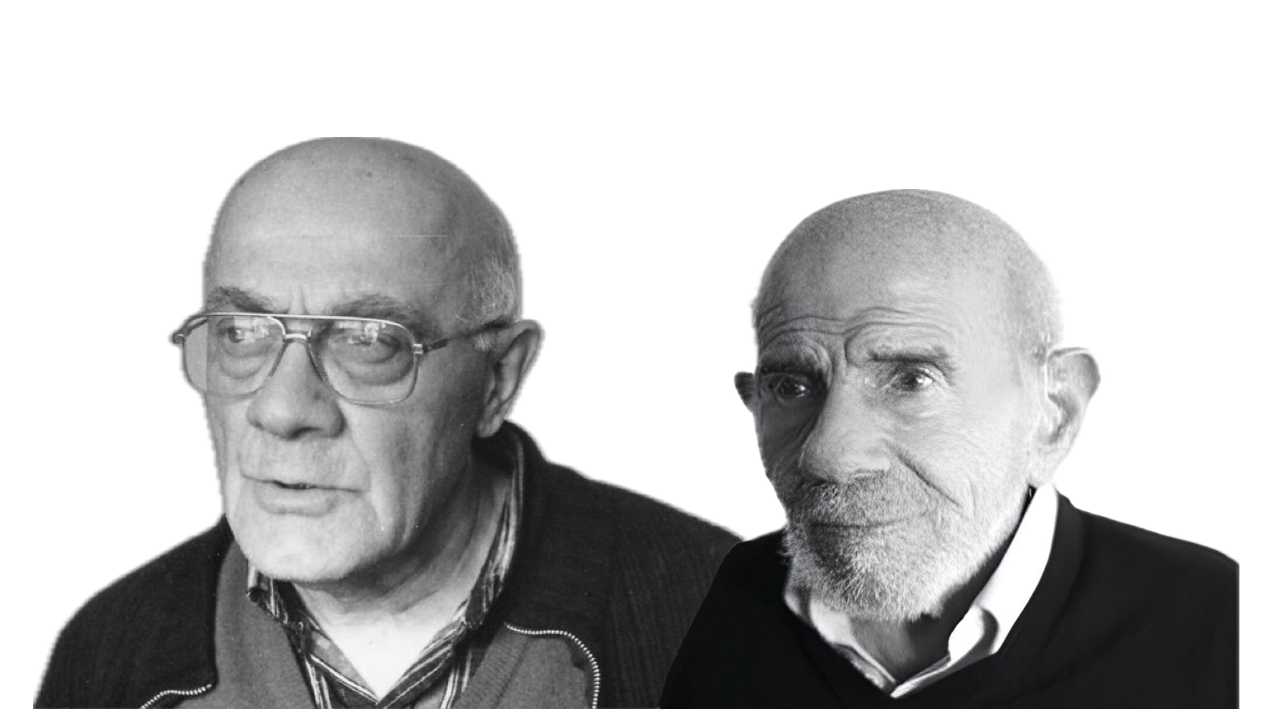
\includegraphics[width=\textwidth,trim=4 4 4 4,clip]{pictures/title.png}
    \vfill
\end{titlepage}

\tableofcontents

\chapter{История и философия науки как научная и учебная дисциплина}
\section{Философия науки, ее объект, предмет и структура. Роль философии в науке }   

\subsection{Философия науки, ее объект и предмет}

% Философия науки (ФН) – философская дисциплина, исследующая структуру научного знания, средство и 
% метода научного познания, а также способы обоснования и развития научного знания.

% В широком смысле, это философская дисциплина, занимающаяся осмыслением места и роли науки в отношении <<человек~—~мир>>.

% В узком смысле — деятельность ученых, посвященная философским и этическим проблемам развития науки.

% Объектом философии науки является наука как социальный и культурный феномен, а её предметом — познавательные структуры и методы, механизмы научного открытия, принципы объяснения и % обоснования научных знаний, а также этические аспекты науки.

Философия науки (ФН) --- философская дисциплина, исследующая структуру научного знания, средство и 
метода научного познания, а также способы обоснования и развития научного знания.

ФН как дисциплина появляется на рубеже 19-20 вв. В западной традиции принято 
использовать понятие эпистемология, но по содержанию это понятие уже, чем ФН, процесс познавательной 
деятельности в науке, ФН шире, структуру.

Объект ФН --- наука как исторически изменчивое единство её важнейших элементов (знание, техника, 
научные институты, типы научной деятельности, субъекты науки). Наука исторична, меняется вместе со 
сменой исторических эпох.
 
Предмет ФН --- наука, рассматриваемая через призму философии данной эпохи и общества. Точка анализа 
науки изменчива исторически, меняется наука и философия науки, который её исследует.

\subsection{Структура философии науки}

\subsubsection{Исследование науки как социокультурного феномена, как вида сознания и знания}

;-)

\subsubsection{Изучение философско-методологических оснований науки}

Онтологические представления о том, 
как устроен мир, гносеологические – методы достижения истинного знания, методологические 
знания -0 какой метод лежит в основе науки.
 
\subsubsection{Анализ проблемы возникновения науки и основных стадий ее развития
}
Существует два подхода к пониманию развития науки. Согласно концепции \textit{континуизма}, наука развивается поступательно и непрерывно, следуя эволюционному ходу. Концепция \textit{дисконтинуизма} утверждает, что развитие науки прерывается научными революциями, после которых она переходит на качественно новый этап с изменёнными фундаментальными представлениями.
    
\subsubsection{Изучение социокультурной динамики науки}

Иначе — определение движущих сил развития науки. Выделяются позиция \textit{экстернализма}, согласно которой основными движущими силами развития науки являются внешние факторы (например, социальный заказ, социальные ожидания от науки), а также позиция \textit{интернализма} - основными движущими силами развития науки являются внутренние факторы (интеллектуальные философские, собственно научные).
    
\subsubsection{Исследование философских проблем областей научного знания} 

Например, проблема жизни. Что такое жизнь с точки зрения различных научных дисциплин? Как эти разные понимания жизни объединяются? Есть ли у физики, биологии, химии, психологии нечто общее в понимании того, что такое жизнь? 

Или проблема происхождения Вселенной. Существовала ли она всегда, либо она появилась в какой-то момент?
        

	\subsection{Функции философии в науке} 

Долгое время обсуждалось, как отделить философию от науки и минимизировать её влияние, вплоть до полного устранения. Однако с конца XIX века, когда философия стала частью профессиональной подготовки ученых, возникла необходимость понять, какую роль она играет в научном образовании. 

Можно выделить несколько функций, которые философия выполняет в рамках научной деятельности.
\begin{itemize}
    \item \textit{Интегративная}. 
    Системное, целостное обобщение разнообразных форм познания, практики и культуры. Создание всеобщего и универсального знания.

    \item \textit{Критическая}. 
    Выяснение границ применимости получаемого человеком знания. Формирует критического сознания.  

    \item \textit{Мировоззренческая}. 
    Разработка определенных моделей реальности, сквозь призму которых ученый смотрит на предмет исследования (например, материализм, идеализм, дуализм)

    \item \textit{Гносеологическая}. 
    Исследование наиболее общих закономерностей познавательного процесса.

    \item \textit{Методологическая}. 
    Создание общенаучных методологических принципов. 
    Например, принцип инструментализма (Галилей) — для получения научного знания необходимо использовать приборы и измерительные инструменты.
    Либо принцип историзма — рассмотрение явления без отрыва от контекста его возникновения, протекания и привязки к определенной эпохе и обществу.
    
    \item \textit{Аксиологическая}. 
    Формирование определенных мировоззренческих и ценностных установок ученого. Это ответ на вопросы: <<зачем заниматься наукой?>>, <<что является в науке главной ценностью?>>, <<какую роль наука выполняет 
    в культуре и в обществе?>>, и т.п.

    \item \textit{Прогностическая}. 
    Разработка идей и представлений, значимость которых обнаруживается на будущих этапах развития науки. 
    Например, принцип атомизма — представление о том, что все твердые тела состоят из мельчайших элементов. Появился еще в античности, долгое время не был востребован в науке, но в 18 веке стал центральной опорой 
    всего корпуса химического знания. 
\end{itemize}
	
	\section {Проблема взаимосвязи философии и науки и основные концепции ее решения}

Еще в период античности возникает вопрос: <<как элементы научного знания взаимосвязаны и взаимодействуют с философией?>>. Рассмотрим концепции взаимосвязи философии и науки.

\subsubsection{Метафизическая концепция}

Появилась в античности усилиями Аристотеля.

Философия - это знание целого, а наука — это знание об отдельных областях действительности.
Философия — это некое состояние ума, которое позволяет рассуждать о предельных основаниях, о бытии, об истине и о ценности, а наука (или эпистема) — это знание, которое можно обосновать с помощью доказательства (например, математическое доказательство). 

Наука включается в рамки философии, так как наука является частным случаем рассуждения о всеобщих основаниях.
Аристотель приводит такое утверждение: все частные <<науки>> возникают из философии (н-р, геометрия, математика, астрономия, биология, география).

\subsubsection{Позитивистская концепция}

Возникла в XIX веке. Основоположник концепции — Огюст Конт. 

Наука — это особый вид познавательной деятельности, являющийся самодостаточным и обладающий приоритетом среди остальных видов познания. 
Это логический вывод из концепции развития общества Конта, где он выделяет три стадии: 
\begin{enumerate}
    \item \textit{теологическая}. Окружающий мир объясняется с точки зрения религиозных представлений (н-р, анимизм, тотемизм, фетишизм);
    \item \textit{метафизическая}. Окружающий мир объясняется с точки зрения философии (период: от античности до XIX века);
    \item \textit{позитивная} (научная). Окружающий мир объясняется с точки зрения науки.
Каждый раз, когда происходит смена этапа развития общества, предыдущий способ объяснения мира не исчезает, но он теряет свой приоритет.
\end{enumerate}

Концепция оказалась продуктивной для развития науки, так как позволила науке выработать собственный строгий методологический инструментарий, благодаря чему в 19-20 веке произошли громкие научные открытия. 
Однако позитивизму не удалось отделить философию от науки — ни в плане научного языка, ни в плане научной методологии, ни в плане мировоззрения. 

\subsubsection{Антиинтеракционизм}

Возник в начале 20 века на фоне Первой Мировой войны (Ж.-П. Сартр, К. Ясперс, Н.А. Бердяев). 

Основные проблемы общества — из-за науки, так как технический прогресс привел к глобальным социальным проблемам (мировая война, массовый голод, эпидемии).
Наука не способна исследовать подлинное бытие, что с точки зрения ряда философских направлений является внутренним миром человека 

\subsubsection{Диалектическая концепция}

Представители — Г. Гегель, Б.М. Кедров, В.С. Степин.

Философия и наука — это разные способы познания, но которые не могут существовать друг без друга. Философия изучает всеобщее, наука изучает частное. При этом философия без науки пуста, но наука без философии слепа.


\section {Наука как предмет прикладных исследований в ХХ веке в контексте научно-технической революции и развития <<большой науки>>}

\subsection{История исследований феномена науки.}

\subsubsection{XIX век. Дискуссия между Фрэнсисом Гальтоном и Альфонсом Декандолем}

Она касалась причин возникновения науки. Гальтон связывал развитие науки с расовыми особенностями, утверждая, что наука была создана исключительно белой расой. Декандоль, напротив, в своей книге «История науки и ученых за два века» (1873) на основе статистического анализа выделил 20 социальных факторов, определяющих развитие науки, таких как развитая система образования, доступ к материальным ресурсам, благоприятный климат и поддержка общественного мнения. Он доказал, что развитие науки зависит от социальных условий, а не от расы.

\subsection{«Большая» и «малая» науки. Основные тенденции развития науки в XX веке. Понятие научно-техничес-кой революции}

С точки зрения Дерека Прайса, основоположника современного прикладного исследования науки, в истории науки было несколько периодов:
\begin{enumerate}
    \item малая наука — разрозненные усилия отдельных людей по познанию окружающего мира (в античности, средневековье и в эпоху Возрождения);
    \item наука — в классическом понимании, возникшая в период нового времени (XVII век);
    \item большая наука (XX век) — характеризуется резким увеличением числа ученых, реализацией больших научных проектов и резким ростом научной информации.
\end{enumerate}
\textbf{Факторами формирования} большой науки являются:
\begin{itemize}
    \item Первая и Вторая мировые войны (высокий спрос на прикладные научные исследования);
    \item возникновение тесной связи науки и государства (глобальные и дорогостоящие научные проекты);
    \item рост роли науки в культуре общества.
\end{itemize}
К \textbf{особенностям большой науки} можно отнести:
\begin{itemize}
    \item резко возросшее число ученых (XVIII век~$\cong 10^3$, XX век~$\cong 10^6$);
    \item рост количества научной информации (в XX веке объем научной информации удваивается с периодом 10-15 лет);
    \item превращение науки в профессиональную деятельность;
    \item научно-техническая революция (в конце 40-х годов XX века);
    \item реализация больших научных проектов.
\end{itemize}

\textbf{Научно-техническая революция} — это коренное преобразование производительных сил общества на основе науки.

\subsection{Комплекс современных дисциплин, изучающих различные аспекты науки}

\subsubsection{Науковедение}

Основоположник — Джон Берналл («Социальная функция науки» — 1938 г.).

Задачей \textit{аналитического} направления науковедения является раскрытие закономерностей развития науки. 

\textit{Нормативное} науковедение занимается разработкой основ совершенствования организации научной деятельности. Нормативное науковедение стремится оптимизировать структуру науки для того, чтобы она работала более эффективно. 

\subsubsection{Социология науки}

Представители — Л. Флек и Р. Мертон.

С точки зрения Л. Флека задача социологии науки — это исследование интеллектуальных коллективов, изучение взаимодействия ученого (как индивида и личности) со своей социальной группой.

С точки зрения Роберта Мертона социология науки изучает универсальные нормы научной деятельности (объективизм, коллективизм и т.д.), или т.н. научный этос. 


\subsubsection{Наукометрия}

Основоположник — В.В. Налимов.

Задача наукометрии — измерить количественные результаты научной деятельности, эффективность как отдельного ученого, так и научного коллектива с целью дальнейшего принятия организационных решений в области науки.

\subsubsection{История науки}

История науки занимается проблемой возникновения и развития феномена науки. Можно выделить несколько уровней исторического исследования феномена науки:
\begin{itemize}
    \item наука в контекст развития общества (н-р, <<почему именно в Древней Греции возникает преднаучное знание?>>);
    \item наука как социокультурного феномена (н-р, история российской науки);
    \item история отдельных наук;
    \item история отдельного открытия, исследователя и т.п.
\end{itemize}

\subsubsection{Психология науки}
Изучает психологические факторы научной деятельности. Среди ее основных задач следующие: 
\begin{itemize}
    \item исследование психологических механизмов производства научных знаний в условиях индивидуальной и коллективной деятельности;
    \item разработка проблем психологической подготовки научных кадров, диагностики и формирования соответственных личностных качеств и установок;
    \item разработка проблем возрастной динамики творчества;
    \item анализ психологических аспектов научных коммуникаций, восприятия и оценки новых идей;
    \item анализ психологических аспектов автоматизации и компьютеризации исследований.
\end{itemize}
По большому счету психология науки занимается психологическим аспектом труда ученых. 

\subsubsection{Hормативно-правовое регулирование научной деятельности}

До конца Второй мировой войны, до так называемого Нюрнбергского трибунала практически не было практики нормативно-правового регулирования труда ученых. 

\texttt{Нюрнбергский кодекс}. Кодекс включает в себя несколько принципов, из которых, например, <<Добровольное согласие испытуемого на медицинский эксперимент>>; <<Интересы индивида преобладают над интересами научного сообщества>>.

\texttt{Хельсинская декларация Всемирной медицинской организации (1964 г.)}. 
Представляет собой набор этических принципов для медицинского сообщества, касающихся экспериментов на людях. Введено разделение на исследования:
\begin{itemize}
    \item c лечебной целью — которые направлены на разработку новых методов лечения или применяются в ситуациях, когда другие способы помочь пациенту невозможны, а его состояние угрожающее.
    \item с теоретической целью — которые изучают особенности работы организма, например, реакции на экстремальные условия (перегрузки, переохлаждение, отсутствие сна), без непосредственного лечебного значения.
\end{itemize}

\texttt{Конвенции о правах человека и биомедицине}. Сформулирован принцип необходимости этических комитетов, осуществляющих независимую экспертизу обоснованности необходимости проведения эксперимента.

\texttt{Декларация о геноме человека и правах человека (ЮНЕСКО)}. В декларации постулируется, что геном человека – основа изначальной общности всех представителей человеческого рода, и он не должен служить источником извлечения доходов. Все геномные исследования должны быть тщательно выверены, их обоснованность не должна вызывать никаких сомнений, и каждое национальное государство обладает своим суверенитетом в деле разрешения или запрещения геномных исследований. 

Наиболее явным образом нормативно-правовое регулирование научной деятельности осуществляется для исследований, направленных на изучение человека (медицинские, физиологические и пр.). Можно ожидать, что со временем начнет регулироваться и научная деятельность как таковая, поскольку современные исследования могут иметь последствия, которые необходимо учитывать в глобальном планировании развития экономики и общества.

\chapter{Многообразие научного знания и его структура}
\section{Различные типы знания. Специфика научного знания и его критерии}  

\subsection{Сущность знания и познания}

\subsubsection{Понятие знания}
 
Знание ~---~ это \textit{проверенный практикой} результат познавательной деятельности, 
форма социальной и индивидуальной памяти. Знание выступает в виде усвоенных понятий, законов,
принципов и так далее.  

Знание можно разделить на две большие группы: 
\begin{itemize}
    \item \textit{знание-умение} (практическое знание, «знание как»). Имеет специфическую проверку (н-р, можно уметь или не уметь кататься на велосипеде, но нельзя
кататься на велосипеде истинно или ложно);
    \item \textit{знание-информация} (<<знание что>>) --- о наличии у предметов каких-то свойств, знание о закономерностях, знание о последовательности действий в той или иной ситуации. Для него характерна проверка на истинность.  
\end{itemize}


Любое знание нуждается в
объективации. В продуктах труда, в технологиях, в социальных институтах, в
произведениях искусства, в текстах. Даже когда мы говорим об индивидуальном
знании, то, которое содержится только в нашей памяти, оно объективируется там в
понятиях, в образах, в воспоминаниях и в других формах.  После своей
объективации знание может быть передано другому человеку.  

Субъект знает некий предмет, если соблюдаются следующие условия:
\begin{itemize}
    \item условие истинности предмета;
    \item условие убежденности/приемлемости;
    \item условие обоснованности.
\end{itemize}


\subsubsection{Понятие познания}

\textit{Познавательная
деятельность} --- это сознательная деятельность субъекта, направленная на
приобретение информации об объектах и явлениях реальной действительности. Это
единство чувственного восприятия, теоретического мышления и практической
деятельности.  

В результате познания формируется
познавательный образ --- образ, возникающий в сознании при непосредственном или
опосредованном взаимодействии субъекта с объектом.  

Познавательные образы делятся на: 

\begin{itemize}
    \item чувственные образы:
    \begin{itemize}
        \item элементарные (ощущение, восприятие и представление);
        \item синтетические (чувственные образы, стереотипы, художественные образы, модельные представления);
    \end{itemize}
    \item рациональные образы (теоретическое восприятие особенностей класса предметов 
через систему всеобщих и необходимых свойств этого класса, выраженных
в понятии):
    \begin{itemize}
        \item элементарные (понятия, термины);
        \item синтетические (совокупность понятий, связанных 
единым смыслом или единой политикой их применения в теории или в гипотезе).
    \end{itemize}
\end{itemize}

\subsection{Особенности научного знания} 

\subsubsection{Системность} 

Наука --- это иерархически организованная система знаний, которая делится на отдельные дисциплины. Изменение значимого элемента в этой системе приводит к постепенному пересмотру всей структуры научного знания (например, переход от физики Ньютона к физике Эйнштейна).

\subsubsection{Объективность} 

Наука стремится изучать предметы и явления так, как они существуют в объективной
реальности. Поэтому знание можно проверять на практике, в эксперименте, в
наблюдении и другими способами. 

\subsubsection{Культурно-историческая обусловленность}

Наука зависит от периода и общества, в котором она развивается. Общие характеристики науки существуют, но они абстрактны. Наука исторически меняется, и современная её версия сильно отличается от науки прошедших эпох, несмотря на общую основу.

\subsubsection{Всеобщность}

Научное знание изучает общие законы и свойства предметов, стремясь формулировать универсальные законы, применимые в любой точке Вселенной. (Хотя и существует гипотеза о возможных исключениях во Вселенной, она остается неподтвержденной.)

\subsubsection{Необходимость}

В научном знании фиксируются системообразующие стороны явлений. 

\subsubsection{Дисциплинарная принадлежность}

Научное знание можно распределить по различным дисциплинам, что представляет собой горизонтальную структуру. Вертикальная структура связана с иерархией уровней. Междисциплинарное знание возникает на стыке дисциплин, но часто приводит к созданию новых дисциплин, таких как физическая химия или эволюционная психология.

\subsubsection{Подтверждение научным сообществом}

В XVII-XVIII вв., когда институт науки только формировался, распространенной практикой было приглашение ученых или уважаемых людей для демонстрации экспериментов, чтобы подтвердить результаты. Если эксперимент не удавался, ученый мог быть подвергнут остракизму. Сегодня существуют институциональные механизмы подтверждения научных результатов, такие как рецензирование и редактирование статей, а также защита диссертаций, которые обеспечивают коллективное признание научных достижений.

\subsection{Научные конструкты и требования к ним}

Объект
исследования, который чаще всего наука изучает, является не самим объектом, а
является конструктом.
\textit{Научный конструкт} --- это умозрительное построение, вводимое гипотетически
и создаваемое по правилам логики. 

К ним выдвигаются следующие требования:
\begin{itemize}
    \item возможность логических операций над конструктами как языковыми выражениями;
    \item множественность связей между конструктами в рамках некоего целого;
    \item устойчивость конструктов (то есть постоянство значений в различных контекстах);
    \item экстраполируемость конструктов (то есть возможности их максимально широкого использования помимо породивших их ситуаций);
    \item согласованность выражений конструктов с установленными закономерностями;
    \item простота конструктов.
\end{itemize}

\subsection{Сравнительная характеристика
научного и обыденного знания}

\begin{longtable}{|>{\raggedright\arraybackslash}p{7cm}|>{\raggedright\arraybackslash}p{7cm}|}
\hline
\textbf{Обыденное знание} & \textbf{Научное знание} \\
\hline
\endfirsthead

\hline
\textbf{Обыденное знание} & \textbf{Научное знание} \\
\hline
\endhead

непрофессиональное, неспециализированное жизненно-практическое, повседневное знание & Продукт специализированной, профессиональной формы человеческой деятельности \\
\hline
не имеет строгого концептуального, логического, системного оформления. & носит теоретический, концептуальный характер; отличается системной организацией \\
\hline
не требует для своего усвоения специального обучения и подготовки & требуется специальное обучение для овладения им\\
\hline
констатация явлений, связей и отношений & ориентировано на поиск закономерностей \\
\hline
может иметь субъективный характер & в идеале должно быть объективным, доказательным, точным \\
\hline
предмет всегда нагляден и доступен восприятию & включает в себя системы абстрактных объектов \\
\hline
дается преимущественно как типичное, понимаемое по аналогии & имеет творческий характер\\
\hline
осуществляется познание единичных ситуаций и явлений & носит универсальный характер \\
\hline
решает конкретные, сиюминутные жизненные проблемы & выходит за рамки практической заинтересованности \\
\hline
использует для фиксации знания устную разговорную традицию &  использует письменную традицию \\
\hline
\end{longtable}


Проблема демаркации научного и обыденного знания остаётся нерешённой, потому что обыденное знание часто предшествует научному. Наука возникает на базе первичных представлений о свойствах объектов, с которыми человек взаимодействует в повседневности. Кроме того, наука использует естественный язык, схожий с тем, который применяется в обыденном знании, хотя стремится к большей формализации. 

В истории были попытки создать строго формализованный научный язык, свободный от недостатков естественного, но полностью это не удалось. Исключение составляет, возможно, математика, которая может быть рассмотрена как формализованный язык. Научный язык и язык обыденного знания связаны через общие понятия и вложенные в них смыслы.



\section{Основные классы научного знания и их дисциплинарная организация} 

\subsection{Проблема классификации науки}

Научное знание может быть классифицировано на определенные
элементы. Проблема классификации наук заключается в том, что в
результате этой классификации необходимо раскрыть взаимосвязи между элементами
науки и выработать представление о ее некой целостной структуре. 

В истории философии были неоднократные попытки классифицировать научное знание. 
Рассмотрим некоторые из них.

\subsubsection{Классификация Аристотеля (384-322 гг. до н.э.)}

Аристотель делил знание на: 

\begin{itemize}
    \item \textit{теоретическое}, где познавательная деятельность ведется ради самого познания. И философия, и наука относятся к теоретическому знанию, занимаясь познаванием из
    отстраненной позиции, пытаясь созерцать явления во всей полноте. 
    \item \textit{практическое}, где познание ведется для выработки идей для поведения человека; К практическому знанию относятся те отрасли, которые
    вырабатывают определенные принципы поведения человека в жизни (повседневной, политической, и т.д.). Например, этика и политика.
    \item \textit{творческое}, где познание осуществляется для достижения чего-либо
    прекрасного. К творческому знанию относятся виды деятельности, направленные на
получение чего-то прекрасного. Например, риторика, поэтика, живопись.
\end{itemize}

В основании классификации положен принцип цели
познавательной деятельности. Данная классификация не приближает к
пониманию специфики науки, определенного класса знания. 

\subsubsection{Классификация Фрэнсиса Бэкона (1561-1626 гг.)}

Науки делятся на: 
\begin{itemize}
    \item \textit{исторические} --- описание фактов (как гражданских, так и естественных);
    \item \textit{теоретические}, или философия в широком смысле слова;
    \item \textit{поэтические} --- литература, искусство, поэзия. 
\end{itemize}

В основании классификации Бекона лежит принцип опоры на определенные
интеллектуальные способности: память, разум или воображение. 
При выборе интеллектуальной способности возникает
класс научного знания. Однако внутри класса трудно провести дальнейшую
спецификацию. 

\subsubsection{Классификация Георга Гегеля (1770-1831 гг.)}

Исходя из своей системы диалектики, он делит знания на три раздела: 
\begin{itemize}
    \item \textit{логика}: учение о бытии, учение о сущности и учение о понятии;
    \item \textit{философия природы}: механика, физика и органическая физика;  
    \item \textit{философия духа}: изучение субъективного духа (человека), объективного духа (общества) и абсолютного духа (Бога). 
\end{itemize}

Система является стройной, и внутреннее деление на дисциплины близко к современной классификации. 

\subsubsection{Классификация Огюста Конта (1798-1857 гг.)}

Им предложена следующая классификация:

\begin{itemize}
    \item математика (вкл. механику);
    \item астрономия;
    \item физика;
    \item химия;
    \item биология;
    \item социология.
\end{itemize}
При движении от математики к социологии
увеличивается сложность предмета исследования: геометрические фигуры, числа, их
взаимодействие наиболее простой предмет исследования, а социальные процессы ---
наиболее сложные. 

В обратную сторону происходит
увеличение абстрактности предмета: у социологии предельно конкретный предмет
исследования, у математики --- предельно абстрактный. 

Предметы исследования в данной классификации достаточно изолированы друг от друга. 

\subsubsection {Классификация Фридриха Энгельса (1820-1895 гг.)} 

\begin{itemize}
    \item механика;
    \item физика;
    \item химия; 
    \item биология; 
    \item социология. 
\end{itemize}

Предметы не изолированы, а
дисциплины означают диалектический переход от одной формы движения материи к другой.
Т.о., социальная форма движения
материи включает в себя остальные формы движения материи, но ими
не определяется по своей природе. 


\subsubsection{Классификация В.И. Вернадского}

Вернадский разделял науки на две категории:
\begin{itemize}
    \item науки, законы которых охватывают всю реальность;
    \item науки, законы которых свойственны только Земле.
\end{itemize}

Эта классификация имеет практическую ценность в рамках концепции Вернадского о развитии планеты и общества. Для Земли характерны уникальные явления, такие как жизнь и разумный человек, которые не найдены в других частях Вселенной. Поэтому науки, изучающие человека и общество, являются уникальными для Земли. Напротив, такие науки, как физика и химия, охватывают всю реальность. 

\subsubsection{Современная классификация наук} 

В современности деление происходит по трем аспектам: предмет исследования, особенности методологии и критерии научности в данной отрасли.
\begin{itemize}
    \item математические науки;
    \item естествознание;
    \item гуманитарные науки;
    \item социальные науки;
    \item технические науки.
\end{itemize}
 
\subsection{Фундаментальное и прикладное научное знание} 

Разделение наук на фундаментальные и прикладные --- еще один вариант классификации, который широко используется, в том числе для повседневного описания науки. 

\subsubsection{Фундаментальная наука}

Это область научного познания, включающая теоретические и экспериментальные исследования
основополагающих явлений. 

Фундаментальная наука характеризуется концептуальной универсальностью и всеобщностью во времени и пространстве. Ее выводы применимы ко всем системам и условиям в любой точке Вселенной и касаются основополагающих явлений, таких как строение материи, энергия, фундаментальные взаимодействия и эволюция Вселенной. 

\subsubsection{Прикладная наука}  

Направлена на интеллектуальное обеспечение инновационного процесса, как основы развития современной цивилизации. Прикладная наука обеспечивает конкурентное преимущество.

Прикладные научные исследования начали развиваться в 19 веке благодаря деятельности Юлиуса фон Либиха, который систематически использовал науку в интересах промышленности, начиная с химической отрасли. 

\subsection{Дисциплинарная структура науки}

Научная дисциплина --- это форма систематизации научного знания.
Она формируется на основе общности объекта исследования, методов, идеалов и норм исследований.  

Для появления научной дисциплины важно не только осознание общности
элементов, но и появление институциональных форм существования научной
дисциплины. 
Кроме этого, в дисциплинарной структуре науки постоянно происходит интеграция и
дифференциация научных дисциплин. 
Дифференциация подразумевает собой появление дисциплин со все более узким предметом
исследования. 
Интеграция, наоборот, означает то, что предмет исследования
расширяется.


\section{Уровни научного познания и соответствующие им методы и формы знания}
 
\subsection{Эмпирический уровень научного познания}

В результате непосредственного или опосредованного контакта с
предметом исследования ученые получают знания об определенных событиях и явлениях. 

\subsubsection{Формы эмпирического знания}

\textbf{Научный факт} --- это форма эмпирического научного знания, в которой фиксируется
некоторое конкретное явление или событие. 
Чтобы факт мог называться научным, необходимо соблюсти следующие требования:
\begin{itemize}
    \item отношение к определенной предметной области науки; 
    \item содержательное описание процедуры и  обстоятельств фиксации события;
    \item усредненность результатов наблюдений и измерений; 
    \item воспроизводимость в научной деятельности  других  исследователей;  
    \item соотношение  с  некоторой  совокупностью, системой родственных или схожих фактов;
    \item теоретическая нагруженность (понятия, с помощью
    которых факт формулируется, соотносится с определенной научной теорией, и в
    рамках этой теории обладают определенным смыслом).
\end{itemize}

Научный факт имеет определенную структуру, состоящую из трех
компонентов:
\begin{itemize}
    \item \textit{перцептивный} компонент --- это чувственный образ, который возникает в
    результате восприятия явления;
    \item \textit{материально-практический} компонент --- это
    совокупность приборов, инструментов и действий с ними, используемых для
    установления факта;
    \item \textit{лингвистический} компонент --- это высказывание, формулирующее факт.
\end{itemize}


\textbf{Эмпирическое обобщение} --- это форма знания, которая фиксирует в
себе некую внешне проявляющуюся причинно-следственную связь. Например, если мы 10 раз уронили бутерброд с маслом, и он каждый раз падал маслом вниз, мы можем сформулировать эмпирическое обобщение, что бутерброды с маслом, вероятно, будут падать маслом вниз. Причины этого явления нам пока неизвестны, но мы зафиксировали внешнее проявление причинно-следственной связи: уроненный бутерброд всегда падал маслом вниз.

\subsubsection{Методы эмпирического знания}

Среди эмпирических методов выделяют наблюдение, эксперимент, сравнение, описание и измерение.

\textit{Эксперимент} --- это метод эмпирического научного
исследования, который подразумевает активное и целенаправленное вмешательство в
протекание изучаемого процесса, в том числе в специально созданных и
контролируемых условиях. 

Научное \textit{наблюдение} предполагает фиксацию некого внешнего изменения того или иного процесса. 

\subsection{Теоретический уровень научного познания}

Теоретическое познание описывает идеальные объекты,
которые, в отличие от реальных объектов, характеризуются конечным числом свойств. 

\subsubsection{Формы эмпирического знания}

К ним относятся проблема, гипотеза, закон и теория.

\texttt{Научная теория} --- это форма теоретического научного знания, содержащая целостное
отображение закономерных и существенных связей определенной области действительности.

Научная теория представляет собой высокий уровень организации научного знания, \textit{включая гипотезы, концепции, закономерности и законы}, которые составляют теорию. Теория --- это квинтэссенция теоретического знания, объясняющая явления в широкой предметной области. 

Например, теория всемирного тяготения не ограничивается падением яблока, а охватывает общие принципы взаимодействия материи. Теория эволюции описывает общий процесс эволюции, а не изменения отдельных видов животных.

Компонентами научной теории являются: 
\begin{itemize}
    \item исходные основания --- фундаментальные понятия, принципы, законы, аксиомы,
    которые являются отправной точкой теоретического исследования объекта;
    \item идеализированный объект --- модель существенных свойств и связи
    изучаемых предметов;
    \item логика теории --- совокупность определенных правил и способов доказательства;
    \item философские установки, социокультурные и ценностные факторы (н-р, элементы картины мира самого ученого);
    \item совокупность утверждений, выводимых из этой теории в качестве следствий.
\end{itemize}

\subsubsection{Методы теоретического знания}

Среди теоретических методов выделяют формализацию, аксиоматический подход, гипотетико-дедуктивный метод, обобщение и идеализацию. 

\textit{Гипотетико-дедуктивный метод} заключается в создании системы дедуктивно связанных между
собой гипотез, из которых выводится утверждение о возможных эмпирических фактах. Далее, в эксперименте или в наблюдении отыскиваются спрогнозированные факты. Если они
обнаружены, то гипотеза косвенно подтверждается.  

\subsection{Метатеоретический уровень научного познания}

На метатеоретическом уровне научного познания вырабатываются идеи и принципы, 
с помощью которых происходит обоснование представлений научной картины мира. 
Они служат одним из условий включения научных знаний в культуру соответствующей 
исторической эпохи. 

\subsubsection{Формы метатеоретического знания}

К ним относятся научная картина мира, научная парадигма, общенаучные принципы и философские основания науки.

\texttt{Философские основания науки} --- это
система философских идей, которые используются для обоснования различных
аспектов научной деятельности. Рассмотрим некоторые основания науки:

\begin{itemize}
    \item \textit{онтологические} --- принятые в данной науке представления о строении окружающего мира;
    \item \textit{гносеологические} --- содержат представление о критериях истинности знания;
    \item \textit{логические} --- содержат представление о той логике, которой нужно оперировать для доказательства;
    \item \textit{аксиологические} --- содержат представление о главных ценностях науки (н-р, получение нового знания, пользы для человека, и т.п.);
    \item {методологические} --- представление о том, с помощью какой методологии мы можем получать истинное научное знание (эксперимент, математическое моделирование, и т.п.).
\end{itemize}

\subsubsection{Методы метатеоретического знания}

К ним относятся методологическая рефлексия и философские методы.

\textit{Философские методы} --- методы познания, которые являются сугубо философскими. 
Например, диалектический метод --- метод рассмотрения
развивающихся явлений через диалектическую логику единства и борьбы
противоположностей, перехода количества в качество и отрицания отрицания.

\textit{Методологическая рефлексия} --- это исследование оснований собственной научной
деятельности с точки зрения общих принципов познавательного процесса. 


\chapter{Социально-коммуникативные аспекты науки}
\section{Коммуникативные аспекты науки} 

\subsection{Понятие коммуникации, статус коммуникации в рамках научной деятельности}

\subsubsection{Понятие коммуникации}

% Например, в английском common, community, communication, однокоренные
% слова, которые означают общий, сообщество, общество и связь, общение, сообщение
% соответственно. 

% Слово коммуникация имеет латинское происхождение. От communico
% делаю общим. 

% Благодаря коммуникации человек развивает мыслительные способности
% объединять свои усилия с другими, чтобы строить цивилизацию. Хотя анатомически
% похожие на нас люди были уже 200 тысяч лет назад. Они обрели культуру, начали
% одеваться, хранить мертвых, оставлять рисунки и так далее. Только 50 тысяч лет
% назад, когда придумали язык и начали общаться. Ну а письменность появилась всего
% 6 тысяч лет назад. Так что это новость в масштабах Вселенной. Ну и огромный наш
% эволюционный скачок. 

Среди определений человеческой коммуникации наиболее
распространены такие варианты, как обмен информацией и общение людей. 

В широком смысле, коммуникация представляет собой связь, взаимодействие,
предполагающее положительное взаимно связывающим некими потоками отношение (???).

Основные отличительные черты человеческой коммуникации:
\begin{itemize}
    \item процесс, который предполагает двух и более участников (при общении с собой --- противопоставление самому себе);
    \item передача опыта, смысла, эмоций, информации и т.д.;
    \item восприятие и интерпретация;
    \item длящийся во времени и требующий времени (для осмысления) процесс;
    \item совместность, осуществление связи между;
    людьми, обычно с целью некого взаимного положительного эффекта, предполагающего
    взаимное духовное развитие, обогащение, понимание.
\end{itemize}

\subsubsection{Статус коммуникации в рамках научной деятельности}

В научной среде коммуникация не должна претендовать на основное место в процессе научной работы. Коммуникация и коллективная работа важны наряду с индивидуальной
деятельностью, только в рамках которой возможно творчество. 

Несомненно, обмен
знаниями и совместное планирование исследования, постановка проблемы, поиск
методов ее решения, обсуждение полученных результатов и так далее, крайне важны
для научно-исследовательской работы.

Творчество, производство нового знания — ядро собственно научной деятельности.
Без творческой составляющей, просто из общения как обмена готовыми мнениями научное знание не
могло бы родиться. 

Согласно исследованиям французских мыслителей
XX века Жиля Делёза и Феликса Гваттари, творчество всегда единично. 

Это означает, что
коммуникация как обмен мнениями может лишь способствовать творчеству, вдохновить
человека, обратить внимание одного на то, что более ясно видится другому с его
точки зрения, но не в силах заменить собой творческий элемент научной
деятельности. 

Макс Вебер утверждал, что помимо коммуникации и творчества,
значимой оказывается и повседневная рутинная работа, не в меньшей
степени обеспечивающая и подготавливающая научное открытие.

Таким образом, коммуникация в научной сфере имеет
достаточно важное значение, однако скорее выполняет вспомогательную и
интегративную функцию, чем играет единственную ведущую роль.


\subsection{Формы и способы коммуникации в научной среде}

Благодаря достижениям техники можно
выделить также и широкий спектр инновационных
возможностей и средств для осуществления профессионального общения.

\begin{table}[h!]
\centering
\begin{tabular}{|p{6cm}|p{6cm}|}
\hline
\textbf{Традиционные} & \textbf{Инновационные} \\ \hline
Личная беседа & Интернет-технологии \\ \hline
Письма & Аудио- и видеоконференцсвязь \\ \hline
Научные публикации & Дистанционные технологии подачи и рецензирования публикаций \\ \hline
Конференции, лекции, теоретические доклады, совещания, съезды & Онлайн-встречи, вебинары \\ \hline
Стажировки, повышение квалификации, совместные праздничные мероприятия & Интерактивные игровые формы: тренинги, модели, неформальные корпоративы \\ \hline
\end{tabular}

\label{table:traditional_vs_innovative}
\end{table}

Личное общение дает больше опыта коммуникации и осуществления
научной деятельности, поскольку при этом участвует несколько каналов восприятия, 
есть возможность физического воспроизведения.

Майкл Полани поднимает важную тему личностного или неявного
знания. Знания обретаются не только в ходе устной или письменной коммуникации.
Ряд знаний, умений,
навыков для профессиональной деятельности обретается лишь в процессе регулярной
практической деятельности, зачастую оседая на бессознательном, интуитивном уровне.

Обычную коммуникацию в целом подразделяют на:
\begin{itemize}
    \item вербальную
        \begin{itemize}
            \item устную: дискуссии, сообщения, участие в конференциях и т.п.;
            \item письменную: статьи, отчеты, книги и т.п;
        \end{itemize}
    \item невербальную: мимика, жесты, взгляд, интонация, поза, темп и тембр речи.
\end{itemize}
Указанные формы выражения играют роль в рамках профессиональной коммуникации, поскольку выражения воспринимаются по-разному в зависимости от сложности конструкций, эмоциональной загруженности,
невербального оформления и соблюдения вежливости.


\subsection{Специфика научного языка}

Для научного языка характерны \textit{термины} (15-20\% научной лексики). Это слова или словосочетания, обозначающие понятия в специальной
области знаний или деятельности, которые стремятся к однозначности и не выражают
экспрессии. Важно, что у терминов есть референт в реальности. 

Большую часть научной лексики (30-40\%) составляют: \textit{абстрактная лексика}
\textit{специальные фразеологизмы}, \textit{клише и стандартные обороты}.

Для научных текстов свойственен академический стиль, имеющий следующие особенности:
\begin{itemize}
    \item логичность, непротиворечивость выражений;
    \item высокий регистр (исключение расхожих фраз, оборотов обыденного языка);
    \item четкость, ясность, умеренная простота конструкций;
    \item точность выражений (отсутствие двузначности, размытых и
    пустых формулировок, полное отражение всей фактической информации);
    \item безличные конструкции (употребление научного <<мы>>);
    \item научная лексика;
    \item аргументированность (доказательность и иллюстративность сформулированных
    положений).
\end{itemize}
Важно уметь отличать его от смежных стилей, соблюдая баланс в рамках официальной научной коммуникации. 

Нельзя также не сказать хотя бы в двух словах о нормах
научной коммуникации, которые  Часть этих моментов мы
рассмотрим подробнее в третьем вопросе сегодняшней темы, потому что они больше
относятся к этическим аспектам. 

\subsection{Нормы научной коммуникации}

Помимо очевидного соблюдения \textit{вежливости},
\textit{непредвзятости} и \textit{аргументированной критики}, к нормам научной коммуникации относятся к культура
цитирования и ответственность за самостоятельность получения и
представление результатов научной деятельности.

\subsubsection{Культура цитирования}

В рамках академического стиля действует следующая культура цитирования: 
\begin{itemize}
    \item принято ссылаться в основном на научные статьи и монографии (до 80\% источников цитирования);
    \item возбраняется ссылаться на неавторитетные и недостоверные источники;
    \item недопустимость плагиата.
\end{itemize}

Генеральная цель науки --- создание нового знания. 
Поскольку новое научное знание  как правило основано на уже созданных представлениях, необходимо соблюдать баланс между опорой на авторитетные источники и творческим элементом собственного исследования. 

\subsubsection{Самостоятельность получения и представление результатов}

% Сравним человека и большие языковые модели.

% Оно
% предполагает, в отличие от животных, прежде всего, рефлексивность в постановку
% вопросов и выход на уровень смысла, то есть осмысление, понимание. Также
% отмечают высокую развитость воображения и речи, когнитивных и коммуникативных
% способностей. 

% При этом интересно, что люди не рождаются с человеческой системой
% восприятия, не владеют языком и не умеют сразу мыслить. Собственно, человеческое
% именно формируется. Изначально у нас есть так называемая лепетная речь. Это
% слоговая непонятная речь детей, которой мы все с двух-трех месяцев начали
% пользоваться. 
% Также в нас заложены потребности выражать свое самоощущение в
% связи с происходящим вокруг и играть, примеривая на себя различные роли.
% Благодаря этим естественным предпосылкам в процессе взросления в среде
% человеческого общения ребенок проходит два фундаментальных кризиса. 

% Появление самосознания и развитие совести. Собственно, умение посмотреть на себя со
% стороны, отделяя я от мира, и внутренний диалог, учитывающий самостоятельность
% других, в горизонте максимально возможного, являются уникальными онтологическими
% особенностями человека, на которых и строится вся специфика его бытия по
% сравнению с другими существами. Развитие мышления и языковые способности
% неразрывно связаны. Переработка изначально лепетной речи в классифицирующие и
% маркирующие вещи события взрослый язык, помогает осваивать абстрактные формы,
% теоретические и оценочные инструменты, логическое, критическое и рефлексивное
% мышление. Безусловно, к творческому, исследующему и преобразующему отношению к
% миру у ребенка есть природная тяга. Однако в процессе взросления они получают
% огромный стимул к совершенствованию именно благодаря развитию речи и
% взаимодействию с другими. И человеческий язык не просто средство передачи
% информации, это многомерная и на большую долю иррациональная система. К тому же
% буквально среда нашего обитания, которая с одной стороны задает схему мышления,
% а с другой открывает возможности понимания смысла различных интерпретаций. Так
% что смоделировать все естество языка через логические операции вряд ли
% получится. На самом деле, задолго до распространения современных генеративных
% нейросетей в дискуссиях о таких мысленных экспериментах, как «Китайская
% комната», «Философские зомби», «Мозг в колбе» и так далее, Джон Сёрль, Сол
% Крипке, Дэвид Чалмерс, Дэниел Дэннет, Ник Бостром и другие аналитические
% философы показали, что антологически машинная речь «речь» может представлять
% собой лишь более или менее удачную имитацию типичного, за которой не стоит опыт,
% понимание, подлинное творчество и здравый смысл. Об этом, опять же, ребят, у нас
% будет еще разговор на последних темах, так что не пугайтесь, что я вам тут
% каких-то имен наговорила, мы позже с ними познакомимся. Но что касается так
% называемых больших языковых моделей, они организованы по принципу токенизации,
% надрабления на морфологические составляющие и комбинирования слов естественного
% языка. Обучение нейросетей для генерации текстов предполагает обработку системы
% огромного массива статей в Википедии, художественной литературы, новостных лент
% и других подобных ресурсов. Например, в обучении ChatGPT3 было включено 600
% гигабайт таких текстов, опубликованных в интернете до 2020 года. Из этих текстов
% выявляются закономерности совместного слова употребления, collocations и
% окончаний с присвоением более высоких коэффициентов в более распространенном
% конструкции. Соответственно, ответ на запрос пользователя, в ответ на запрос
% пользователя, выученная таким образом нейросеть, будет выдавать стереотипные
% фразы общими словами. Искусственно-интеллектуальные системы не понимают смысл ни
% запросов, ни своих ответов, ни той информации, на которой их обучили, ни того
% контекста, в котором ведется поиск. Поэтому актуализируются проблемы
% достоверности выдуваемых сведений, этичности содержания, логичности и
% соответствия здравому смыслу. То есть в отсутствии реального, критического,
% рефлексивного мышления, ответы генеративных нейросетей могут противоречить сами
% себе, быть предвзятыми, предоставлять вымышленные или несоответствующие
% действительности данные. К примеру, в ответ на вопрос, сколько минут следует
% варить 3 яйца, если 5 яиц варятся 10 минут, система выдаст 6 минут, что будет
% ошибкой здравого смысла. Или, к примеру, чат GPT считает, что у лошади 8 ног.
% Две правые, две левые, две передние, две задние. Я недавно спрашивала, Яндекс
% Алиса, например, полагает, что в ноябре только один вторник. Ну, то есть
% понятно, какие проблемы с ними возникают. Таким образом, говоря об
% онтологическом статусе, подчеркнем, что нейронная сеть это математическая
% модель, построенная на перцептронах, которые состоят из трех видов элементов.
% Принимающих сигнал, анализирующих его и выдающих реакцию. То есть какой-то
% ответ. Собственно, почему говорят о ненадежности результатов работы нейросетей и
% о том, что их сложно проверить, что они работают как черный ящик. В многослойных
% системах огромное количество таких перцептронов и не обязательно элементарных.
% На каждом из них, из этих миллиардов элементов, в каждом слое выполняется
% настолько много операций, что поиск узла, в котором, например, произошла ошибка,
% вручную просто нецелесообразен с точки зрения затрат времени и ресурсов. Обычно
% в случаях, когда нейросеть плохо обучилась, разработчики отправляют ее на
% переобучение, корректируя выбор, критерии и так далее. Но, естественно, любая
% выборка конечна и не сможет вместить в себя всю полноту реальности, с которой
% этой системе затем придется иметь дело. У нее нет воображения, поэтому она сама
% не сможет ничего оценивать. Она просто производит операции с блоками информации,
% у нее отсутствует выход в пространство абстрактных форм. Так, несмотря на
% некоторые биологические аналогии с работой нервных клеток, нейросети не являются
% живыми, это лишь инструмент работы с большими данными, пусть и сложный по своей
% архитектуре, и ресурсоемкий в плане воплощения в железе. У ныне распространенных
% искусственных систем отсутствует такая базовая характеристика всего
% одушевленного, как наличие воли. То есть нейросеть ничего не делает сама. За ее
% функционирование и использование могут отвечать только люди, разработчики,
% собственники и пользователи. Таким образом, применение генеративных нейросетей
% оправдано, к примеру, в случаях оптимизации рутинной работы, то есть
% автоматизации каких-то шаблонных действий или индуктивного обобщения. Но нужно
% ограничивать или осознанно контролировать их использование в случаях принятия
% экзистенциальных и этических решений, поскольку нейросети не способны осмыслять.
% И создание уникального творческого продукта, которым, например, является научная
% статья. 
Помимо проблемы плагиата, этот вопрос можно рассмотреть в контексте появившихся недавно нейросетей. Выделим следующие принципы использования нейросетей в научной деятельности и коммуникации:
\begin{itemize}
    \item недопустимо применение для обмана, оскорбления, подлога или искажения данных;
    \item недопустимо использовать при требовании самостоятельной работы;
    \item недопустимо применение в области принятия этических и экзистенциальных решений;
    \item декларировать использование, указывать объемы и аспекты применения.
\end{itemize}

\subsection{Коммуникация в сфере науки как ценность}

Наряду с ценностями самого научного знания (истинность, рациональность, общедоступность и др.), коммуникация в научной среде сама обладает огромной ценностью, поскольку:
\begin{itemize}
    \item является живой средой формирования и функционирования научного знания
    (научное знание выражается в языке, распространяется в среде);
    \item позволяет делиться опытом (обсуждение обогащает пониманием специфики исследования, позволяет учиться на чужих ошибках, подчеркнуть позитивный опыт);
    \item дает возможность рассмотреть проблему с различных точек зрения;
    \item высвечивает новые перспективы и вопросы;
    \item побуждает участников точно и ясно формулировать свои идеи.
\end{itemize}
Важно осуществлять коммуникацию в сфере науки на международном уровне,
поскольку воспитанные в разных традициях, коллеги из разных стран могут дополнять друг 
друга и совместно находить решения общих проблем, помогать друг другу в научных исследованиях, которые имеют общечеловеческую ценность. 


\section{Наука как социальный институт.}

\subsection{!!! Индивидуальное и социальное. Профессия и призвание}

Для категориальной пары <<индивидуальное и социальное>> существуют синонимы: 
<<уникальное и универсальное>>, <<частное и общественное>>, <<личное и коллективное>>.
 
В каждом человеке одновременно равноправно присутствуют оба эти
полюса противоположностей. Ни социальное само по себе, ни индивидуальное само
по себе не первично, т.о. не определяют человека полностью. Проблемой является понимание, где и как пролегает граница между индивидуальным и социальным в каждом человеке. 

% К примеру,
% реальную память конкретного человека нельзя называть в полной мере ни
% исключительно его собственной, ни абсолютно коллективно сформированной. С одной
% стороны, на восприятие и запоминание событий влияет множество других людей, в
% том числе косвенно, например, через художественное произведение, а с другой
% восприятие и запоминание являются уникальными актами осмысления, которые человек
% может совершать лишь в индивидуальном порядке, сам, в своей голове, в
% собственном состоянии переживания. Тем не менее, благодаря общению с другими,
% человек способен хранить память даже о событиях современником, которых он не
% был. Поэтому, как бы личностно ни была осмыслена, такая, например, историческая
% информация, невозможно говорить и о том, что она сформировалась человеком
% исключительно индивидуально, без влияния контекстуальной среды, которую
% производят другие. 


Прежде всего, когда мы говорим о человеческом
обществе, мы имеем в виду не только популяцию, набор сосуществующих друг с
другом особей одного вида, иначе нам бы не потребовалась специальная наука
социология, достаточно было бы биологии. 

Казалось бы, очевидно, что человеческое
общество невозможно без другого, или, что, по сути, говорят в том же самом, без
отношения к другому. Но, давайте всмотримся в этот очень тривиальный, на первый
взгляд, простой и даже наивный тезис. 

Интересно, что структура другого, во-
первых, не дана нам изначально от рождения, а во-вторых, формируется сначала во
внутреннем измерении, затем уже как бы экстраполируется на внешних других. 

% Так,
% каждый из нас во взрослом возрасте может быть другим, сам по отношению к себе.
% Ведь каждому известно явление внутреннего диалога, общения с самим собой,
% которое не было бы возможно не быть в человеческом существе, так сказать,
% дублера-наблюдателя, который, например, винит за тот или иной поступок или
% оправдывает себя перед собой, требует отчета о причинах принятия того или иного
% жизненного решения, анализирует произошедшее с собой в прошлом, планирует
% действия на будущее и много еще о чем с собой разговаривает, смотрит на себя со
% стороны, простирается мыслью, охватывая и свои текущие действия, и временные
% модусы прошлого и будущего, и воображение иных пространств и образов, которых в
% эмпирии здесь и сейчас нет. 

% Если говорить упрощенно, я, как здесь и сейчас
% эмпирически поступающее и нечто ощущающее существо, могу не совпадать с собой,
% как существо мыслящим, которое свои действия, поступки, ощущения и соображения
% рефлексирует. Когда мы были маленькими детьми, изначально мир представлял для
% нас как бы сплошной спектр различных состояний, такой калейдоскоп меняющегося
% положения дел и внутреннего самоощущения в связи с этими изменениями. Мы
% отвечали тому, что нас захватывает всей полнотой своего существа, осваивали
% действительность, представляя и как бы населяя все собой. Могли увидеть в
% обычных предметах метафорически другие вещи и играли во все, примеривали на себя
% любые роли.
% От избытка этого опыта и постепенного научения взрослому языку в
% какой-то момент в возрасте двух-трех лет на нас обрушивается серия открытий,
% прежде всего отдельности себя и мира. И у нас впервые устанавливается
% человеческая система восприятия. Мы понимаем, что мир гораздо больше, чем то,
% что мы видим здесь и сейчас. Для нас включается восприятие хронологического
% времени и самое главное мы обретаем самосознание, то есть начинаем отчетливо
% понимать. Вот я и вот все остальное. Я отдельно, я сам, вот я. Нам становится
% многое непонятно, как устроен мир, на чем это все держится, если я отдельно и
% мир не создан. 
% И начинается период вопросов или почемучек. Мы начинаем задавать
% много вопросов. Вот так в нас устанавливается структура другого. Я сам себе
% другой, потому что вот я, тот, кто эмпирически здесь и сейчас, и тут же я на
% него смотрю со стороны и понимаю, что это я, думаю о я. Это возвратное к себе
% движение и называется рефлексией, буквально складывание удвоения, которое
% начинается с отождествования себя с собой и одновременно понимание различия себя
% и мира. 
% Ну и вот этот внутренний ревизор с двух-трех лет будет в нас развиваться
% и в период от четырех до шести мы переживем второй кризис, когда станет
% окончательно понятно, что у каждого отдельного другого человека свое видение
% мира, свое воображение в голове и прямого доступа мне туда нет. Да еще и видеть
% одни и те же события мира мы можем по-разному. Так необходимо будет развивать
% совесть, буквально совместное ведание, то есть я что-то знаю, вижу, мне что-то
% дано и что-то я должен с этим знанием делать, как-то поступать в его свете так,
% чтобы согласовывать свои действия с внешними другими, чтобы и мне было хорошо и
% им. 
Тогда получается интересная неожиданная вещь. Действительно ассоциальность,
а не та, которую мы в обыденном понимании интуитивно предполагаем за этим словом
включает в себя и внутреннее пространство человека в той мере, в какой он
отстоит сам от себя, сам для себя является другим и с этим другим выстраивает
отношения неизбежно совместного бытия. От другого внутри себя уже никак не
отделаться и не отселиться, как это можно было бы устроить физически по
отношению к другим людям. 

% Именно поэтому в частности очень важно быть в единстве
% с собой, в согласии, со своей совестью. если мы осознанно плохо или неправильно
% поступили, соврали, например, то нам придется помнить об этом, чтобы для других
% не раскрылся наш проступок. Но это означает, что мы будем расслаиваться с собой.
% Одна часть нас знает о вранье, а вторая его скрывает и следит за тем, чтобы оно
% не раскрылось. То же самое происходит с завистью, страхом, обидой и многими
% подобными нашими деструктивными переживаниями, которые уводят от единства с
% собой. Поэтому важно их преодолевать в себе. Кроме того, мы представляем в
% голове наши связи, отношения с внешними другими и это очень сильно влияет на
% наши поступки в действительности и на взаимодействие с реальными людьми.

Так что
можно сказать, что каждый носит прежде всего в себе внутреннюю социальность и
как бы через призму внутренних оценок, своих представлений, к тому же меняющихся
у нас в течение жизни, встраиваться во внешние коллективы, группы, коммуникации.
Естественно, наши идеализированные представления о других и о себе, различные
надежды и ожидания часто не оправдываются на деле. Видимо, из-за этого
человеческие отношения такие сложные и в обществе происходят неоднозначные
феномены. Действует прослойка или экран осмысления. Мы не просто повторяем,
воспроизводим тысячелетиями сложившиеся иерархии и все эти связи с другими, мы
можем поставить под вопрос необходимость именно такого социального уклада и
предположить, что другое, более действенное, удобное, правильное, на наш взгляд.

Отсюда возникает история человечества, как трансформация социальных порядков,
опирающаяся на изменения в понимании человека мира и своего места в нем. 

% Приведу пример известного эксперимента с обезьянами. В клетку поместили пять макак,
% подвесили к потолку банан, подставили к нему лестницу. Как только какая-либо из
% макак пыталась забраться за бананом, остальных четверых из шланга поливали
% холодной водой. Неприятная штука, согласитесь? Через некоторое время макаки
% смекнули, что если никого не пускать на лестницу, то никто не будет облит. В их
% сообществе появилась такая норма поведения стаскивать с лестницы, не пускать на
% нее любого, кто попытается взобраться за бананом. Далее в клетке стали по
% очереди менять по одной макаке на новую. Каждый новый член этого сообщества,
% завидев под потолком банан, пытался взобраться за ним. Остальные его стаскивали
% и не пускали. Заменив постепенно всех макак, ученые наблюдали сохранение этого
% порядка, хотя ни одна из этих новых пяти не присутствовала при обливании водой,
% за попытку достать банан, никто за ним не лез, поскольку все друг друга от этого
% удерживали. В принципе, напоминает человеческое общество и передача стереотипов,
% да, ведь? Контрольный вопрос, что отличает человека. 

% В обществе люди всегда
% задаются вопросами о смысле происходящего, о смысле установленных порядков и в
% своей голове прикидывают, как может быть и что будет, если мы так сделаем. это
% не значит, что человек лучше или выше животных, на самом деле, во многом мы
% более ущербный вид, чем остальные, но это говорит о специфике, особенности
% именно человека. Для нас все завязано на осмыслении, понимании. Удивительно, что
% мы не рождаемся уже говорящими на человеческом языке, понимающими смысл из такой
% вот системы восприятия, построенной на другого, на структуре другого, ну или
% структуре различия как такового. 

Что делает
каждого из нас собой? Индивидуальным не является то, что каждый разделяет с другими
внешними людьми, например, верование, представление о мире, моральные нормы, в
которых мы соглашаемся с другими, которые перенимаем от них.Поскольку это вещи
внешние, они могли бы быть другими. 

А вот что в нас не иное? В чем проявляется
индивидуальность? То есть, что в каждом из нас неделимо и от каждого неотделимо?
Своё собственное, не иное. Отличает от всего другого и всех других, но
безусловно, это не собственность в обыденном смысле, поскольку вещи юридической
принадлежности не определяют собственно человека. Их можно полностью поменять,
но от этого не изменится своё. 

Интуитивно кажется, что может быть ближе и
роднее, чем своё собственное тело. Однако, процессы в теле, наши гормоны, гены,
физиологические особенности не детерминируют нас. Многое делается напротив,
вопреки как внешним обстоятельствам, так и внутренним условиям. Все клетки тела
обновляются, меняются каждые 7-10 лет, но мы остаёмся собой. Материи, из которой
мы сделаны, форма, в смысле генетически заложена, единят нас с другими,
обеспечивая семейные сходства и принадлежат к одному роду. Время, в котором мы
живём, пространство, которое занимаем тоже максимально общие универсальные
формы, скорее мы принадлежим им, чем они наша собственность. 

Тогда возможно
собственно своё обеспечивается не чем-то одним, но набором особенностей. В конце
концов уникальность для каждого человека отпечатки пальцев, строения роговицы,
память, точка зрения, особенности характера, способности, интересы, жизненный
опыт поступки. Также и у каждой даже внешне не похожей на другую вазы на деле
уникальное окрашивание, чуть различные составы, форма, трещинские звук при
постукивании. Что уж говорить о гораздо большем числе специфических черт у
животных и растений. 

Возьмёмся определить таким образом собственно своё,
например, конкретного кота. Опишем внешность повадки, предпочтения, назовём имя
собственное и все применяемые к нему уменьшено ласкательное и перечислим события
его жизни, с чем имел дело, как на что реагировал, как опыт усвоил и в этом своё
ускользает. Почему? Кота можно приучить к другому. В новой среде он будет вести
себя не так, как обычно. На какие-то вещи даже знакомые спонтанные иначе иногда
реагировать, но при этом останется собой. Все эти вещи окажутся набором
проявлений его индивидуальности, но не ей самой. 

У человека тем более могут
полностью измениться привычки, в экстремальных условиях он выдаст иной раз, чего
даже сам от себя не ожидал, он может изменить имя, скорректировать характер и
внешность. Кроме того, полнота описания невозможны. Детали, нюансы и потенции
можно перечислять бесконечно, бесконечно углубляться в подробности, но это не
исчерпает сущности определяемого. Когда мы теряемся перед этими парадоксами
своего собственного, перед неприступностью того, что уникально, нам может начать
казаться, что все могло бы быть иным, то есть, что все изменчиво и заменяемо. 

Но
на самом деле свое уникальное безусловно есть, обеспечено самим фактом
существования каждого отдельного и изменчивым его не назовешь, потому что если
бы оно изменялось, мы бы не оставались собой. 

% Мы с вами, ребят, специально
% уделяем внимание рассмотрению парадоксов или опорий, потому что они окружают
% самые значимые вещи, смыслы жизненные, такие, без понимания которых нам плохо,
% без понимания которых мы не чувствуем себя полноценно и свободно. Поэтому нужно
% научить с ними дело, чтобы действительно понять, а не сорваться в
% конструирование схемы, в которой для непротиворечивости утверждается одна часть
% и игнорируется другая. Надо научиться спокойно принимать реальность во всей
% полноте, а реальные феномены всегда противоречивы, тогда мы учимся не сужать
% свое зрение, а смотреть как можно шире, потому что только во всем размахе
% реальное можно действительно увидеть. 

Так вот, что означает этот ход принять
парадокс в нашем случае, когда мы ищем свое собственное? Этот шаг принять, что
мы не знаем свое, но незнание своего, невозможность его концептуализации не
означает, что оно нам недоступно, ведь мы и так без нашего желание от рождения
сами свои уникальные есть. То есть, я могу только быть собой, но знание о том,
что делает меня мной, невозможно. Почему знание об уникальном невозможно? Чисто
логически, ребят, смотрите, в знании мы схватываем универсальное, общее, для
ряда похожих, но на деле единичных предметов или явлений, а об уникальном знание
просто не может быть, потому что оно противоположно универсальному и это
нормально. Никто бы из нас, наверное, не хотел, чтобы о нашей индивидуальности
было доступно всем знание и оно бы нас полностью детерминировало, значит,
закрепощало бы, повязывало бы по рукам и ногам, а мы свободны. Кстати,
этимологически свое и свобода слова одного происхождения и не будет в принципе,
даже если кто захочет, ограничивающего знания об индивидах. 

Еще раз смотрите,
какой здесь ход. любая попытка уловить свое является смотрением со стороны,
поэтому неизбежно оборачиваться разделением, противопоставлением себя, самому
себе, а значит, потерей единства, которое только и может хоть как-то приблизить
к своему, потому что индивид это неделимое по определению. 

% выдающийся
% отечественным мыслителем Мирам Константин Шмамар Дашвили по этому поводу
% приводят следующую показательную аналогию. Процитирую вам из его книги «Эстетика
% мышления». Мы ведь в зеркале себя не видим, а видим себя смотрящего в зеркало. И
% точно так же в наших идеологических представлениях, в идеологических частях
% сознания мы не видим себя вовсе. Мы видим кого-то, имеющего о себе, такие-то
% представления и так на себя смотрящего. Это не мы сами. Невозможно засечь себя
% не смотрящим в зеркало. Извне тоже никто не скажет достоверно о нашем собственно
% своем, так как не дано быть за другого. Другой не может влезть в мою шкуру и за
% меня что-то подумать, почувствовать или пережить моим способом. Надеюсь, на этом
% примере разбора парадоксов своего собственного вы видите, где заканчивается
% территория науки и начинается территория философии. 

Есть такие сферы бытия, в
которых знание невозможно или не действует. Даже если мы его составим, например,
об этом конкретном котике, оно не будет иметь ценности, потому что вся прелесть
его в том, что он сам самобытный, самостоятельный и с долей спонтанности. Все
это, естественно, не означает, что о таких вещах не нужно говорить. Напротив,
ведь, конечно, каждый хочет найти себя, понять, что именно его свое собственное.
Сделать это трудно еще и потому что со всех сторон другие спешат нам указать,
кто мы такие и чем должны заниматься. Мы не доверимся социальным стереотипам, не
пойдем в данном случае по пути предлагаемым коллективам, потому что ищем
противоположное, индивидуальное, свое. Тогда берем философский инструментарий и
продолжаем мужественно в такие вещи все равно самостоятельно всматриваться, как
они нам являются. То есть, пусть в своей глубинной сущности они не преступны, но
какими-то сторонами к нам поворачиваются через что мы имеем с ними дело, в чем
они нам доступны, в каких аспектах открываются. Пребывая при своем собственном
или исполняясь в собственном своем, мы совпадаем с собой. В таком состоянии в
нас как бы выключается дублер-наблюдатель, мы перестаем смотреть на себя со
стороны и становится неважно, как мы выглядим, правильно ли делаем то, чему
отдали здесь и сейчас, что было до этого и что будет потом. То есть, исчезают
также страхи и желания. Это состояние можно назвать «меня нет». Оно связано с
определенным отключением от восприятия себя. Например, когда нас что-то
захватило, мы в какой-то момент перестаем замечать, что у нас что-то болит,
когда до этого болело, или долгое время не чувствуем голода. То есть, нам не
мешают представления о себе, контролирование себя, они как-то растворяются и не
отвлекают. И этому сопутствует чувство единения со всем миром, чувствуется
одиночество, даже если человек в этот момент не среди других людей. Мы всем
своим существом пребываем здесь и сейчас, не рассеиваясь ни на сопоставление с
другими, ни на представление неприсутствующих непосредственно перед нами
пространств, не копаемся в прошлом и не строим планы на будущее. Мы целиком
концентрируемся в моменте «теперь». А он единственное, настоящее, реальное,
подлинное. Ведь прошлого уже нет, а будущего еще нет. И даже если мы их
представляем, они лишь возможности у нас в голове. А концентрация на том, что
непосредственно сейчас дает максимальную полноту действительности. Это
счастливое состояние. Не случайно в языке есть поговорка «счастливые часов не
наблюдают». В экстазе полноты исполнения исчезает восприятие времени. Занимаясь
чем, мы перестаем замечать течение времени. Это может быть все, что угодно.
Прогулка и наслаждение пейзажем, пребывание рядом с любимым человеком,
воспитание детей, осмысление чего-то важного, игра, интересная работа, чтение,
просмотр фильма, уборка, слушание музыки и так далее. Общее в этих моментах
состояние захваченности, когда мы отдаемся полностью вплоть до самозабвения.
Парадокс в том, что мы по-настоящему обретаем себя, только отдав себя
захватывающему чему-то исполняемся, то есть достигаем интенсивной полноты своей
жизни, что позволяет нам взять свою максимальную амплитуду в данных условиях.


Таким образом, индивидуальность каждого предполагает разворачивание своего
собственного данного нам отрождения уникального угла зрения. Никто другой в моей
шкуре за меня так видеть, переживать, осмыслять не может. И в свете этого зрения
уникального набора способностей, интенсий, склонностей. 

Наконец, пометим главный
критерий своего. Это то, что мы не можем не делать, чем бы ни занимались.
Например, кто-то может во всем видеть сложные задачи и исполняться в том, чтобы
их решать, все вокруг оптимизировать. Кто-то не может без коммуникации общаться
с другими, помогать им советом, поддерживать, делиться информацией, выстраивать
связи и в том числе вести с собой диалог. Кому-то обязательно надо что-то новое
придумывать, критерий, ведь даже в обыденных рутинных делах кого-то тянет все
упорядочиво, систематизировать, тщательно, аккуратно выполнять, пусть и
обыденные рутинные процедуры, но доводя любое дело не до совершенства. 

Свое собственное каждый человек может развернуть на
любом содержании, в любом делании. Этим-то призвание и отличается от профессии.

Профессия имеет содержательное наполнение, то есть, что человек делает? 

В то время, как призвание
основано на уникальном способе быть, поступать, видеть, думать, то есть, как
человек делает, важно, что именно. 

% Говоря о самореализации, это, напомню,
% согласно пирамиде Маслоу, высшая потребность человека, без удовлетворения
% которой он в полной мере не будет чувствовать себя счастливым, многие начинают
% ошибочно полагать, что стоит мне подобрать профессию по душе, как я буду
% абсолютно счастлив. Но ошибочность такого мнения должны указать следующее
% соображение. Во-первых, дети счастливы без какой-либо профессии, более того,
% постоянно примеривают на себя разные роли и захватывать могут одинаково
% постройка крепости и ухаживание за больными в кавычках куклами. Во-вторых,
% предположим, человеку больше всего приносит смысл производство обуви, научные
% исследования в области химии или продаж товаров. Даже если человек реализуется в
% любимом занятии, в его жизни остается время, когда его отвлекают, приходится
% делать рутинные вещи или нужно переключиться на что-то иное, в том числе на
% отдых. Следовательно, он не будет полностью все время своей жизни счастлив своим
% собственным, если понимает его содержательно. Иначе проходит жизнь человека,
% когда он видит, что его свое собственное не зависит от содержания того, чем он
% занимается, а исполняться можно в каждом проживаемом мгновении. Например,
% креативить и находить нестандартные решения можно во всем, от сочинения музыки
% до паяния микросхем, от разработки нового метода синтеза до участия в играх.
% Так, только разглядев в себе свой способ бытия, можно быть счастливым каждое
% мгновение, концентрируясь на том, что здесь и сейчас, применяя себя, осуществляя
% свое бытие на материале любых содержаний. И вот, когда человек ощутил на себе
% эту истину, я могу исполниться в чем угодно, проявить себя в любом деле, суметь
% применить свои способности даже в том, что не нравится содержанию, тогда он как
% бы укореняется в бытие, перестает быть потерянным или растерянным, неуверенным,
% обретает себя и свое место в мире, а значит, и устойчиво встраивается в
% взаимоотношения с другими людьми. И если в этом ключе глянуть на игру
% социального и индивидуального в научной деятельности, то нетрудно заметить, что
% хорошие, продуктивные коллективы исследователей, которые качественно и
% ответственно подходят к своей работе, выстраиваются только вокруг людей,
% которые, вопреки каким-то внешним негативным обстоятельствам и неудачам,
% мужественно продолжают идти к свету истины, которые стараются на этом
% профессиональном поприще максимально развернуть и применить свои способности, а
% также учиться новому. Конечно, не все, кто приходит в науку, являются со
% стереотипной точки зрения учеными до мозга костей, но это не беда, ведь каждый
% может смотреться в себя, осмыслить свои уникальные склонности и способности,
% которые можно было бы применить в рамках профессии ученого. Кому-то нравится
% кропотливая работа руками, например, в химии проводить точно и аккуратно
% аналитические процедуры или организовать синтез веществ разнообразными
% способами. Кто-то, напротив, меньше любит работать руками или возиться с
% приборами, но его хлебом не кормит, дай только что-нибудь рассчитать, решить
% какие-то сложные интеллектуальные задачи, представить цифры, данные в виде схемы
% таблиц. Третье, больше любит рассуждать теоретически, пытаясь подобрать какие-то
% аналогии, помогающие представить, скажем, механизм реакции или тот или иной
% эффект транспортных свойств твердого тела. Четвертое, любит работать с текстами,
% систематизировать данные, интерпретировать, выражать научные идеи в языке,
% переводить зарубежные статьи, выступать на конференциях. А пятый, мало что,
% спосвящий в этих всех тонкостях, просто хороший управленец, руководитель,
% который может этих четверых организовать, помочь им раздобыть реактивы,
% договориться о проведении серии экспериментов в сторонней организации,
% проконтролировать техника, чтобы вовремя починил прибор, пробить источник
% финансирования, убедить руководителей на производстве, купить в свою группу
% разработку и так далее. Конечно, это идеальный коллектив, в котором каждый
% находит себе место по призыванию, каждый имеет возможность реализовать свои
% способности. В таком коллективе обычно, когда люди заняты каждым своим делом,
% царит атмосфера взаимопонимания и взаимной поддержки, и даже если возникает
% разумево, все спокойно обсуждается и решается разумом. Притом интересно, что
% такие коллективы могут складываться вовсе не обязательно на базе одного отдела
% или одной лаборатории, это могут быть люди из разных структурных подразделений,
% организаций, из разных организаций, из разных городов и даже стран. Однако,
% человек не на месте, когда ему не дают проявлять свое собственное, реализовывать
% свой потенциал, или же он сам не разглядел в себе те способности, которые можно
% в данных условиях продуктивно применить, человек чувствует себя несчастливым и
% частенько возникают всякого рода перекосы. Кто-то становится агрессивным по
% отношению к другим, постоянно провоцирует конфликтные ситуации, пускает сплетни
% или наоборот, он замыкается в себе, теряет интерес к работе и к жизни, впадает в
% депрессию. Поэтому очень важно в социальном плане внуки, чтобы максимально
% исполниться, во-первых, научиться всматриваться в свое собственное, что
% называется, найти себя, а во-вторых, уметь видеть эту социальную ткань вокруг
% себя, чтобы встроиться в нужную именно вам констелляцию отношений. И если на
% текущем рабочем месте вы чувствуете такой социальный дискомфорт, это вовсе не
% значит, что нужно уходить с этой работы или бросать науку. В любой сфере
% коллективы разные и везде вы встретите как деятельных людей, так и тех, кто не
% нашел себя и поэтому мешает другим. Надо искать свое место, выстраивая настоящие
% человеческие связи с теми людьми, которым вы чувствуете тягу, присматривайтесь
% друг к другу, предлагайте интересно, на ваш взгляд, ученым провести совместные
% исследования, связывайте знакомства на конференциях, посещайте какие-то
% обучения, стажировки, научные мероприятия и кто знает, может быть, ваши
% настоящие соратники, с которыми вы образуете удачный коллектив уже рядом. 

\subsection{Социологические исследования научной деятельности}

Исследования в области социологии научной деятельности проходят на трех уровнях:
\begin{itemize}
    \item микроуровень (исследование научных коллективов: их формирование,
    управление ими, распределение ролей, сеть связей вокруг учёного, призвание и профессия);
    \item мезоуровень (как наука существует в государстве, в каких организациях занимаются наукой и т.д.);
    \item макроуровень (какова внутренняя структура научных учреждений и иерархия их соподчинения, как происходит воспроизводство научных кадров).
\end{itemize}

\subsubsection{Теория Роберта Мертона} 

Роберт Мертон считал, что ученые, получившие
признание коллег на ранних этапах научной карьеры, имеют в дальнейшем гораздо
больше шансов к продвижению своих идей, публикации работ, дополнительному
финансированию и т.д., по сравнению с исследователями, которые медленнее
набирают обороты или на этапе обучения не были высоко оценены старшими
коллегами. Эта закономерность получила название \textit{эффекта Матфея}.

Внимательно рассматривая эту теорию, можно заметить, что данный эффек верен лишь на
уровне социального стереотипа. 
В действительности известны прямо противоположные случаи, когда,
вопреки именно неблагоприятным условиям, и в отсутствии раннего проявления
способностей вырастает настоящий.

\subsubsection{Акторная сетевая теория Бруно Латура}

Основная идея Латура в том, что продукт научной деятельности создается как ученными, 
так и множеством сопутствующих акторов (среди которых, н-р, рецензенты, поставщики 
материалов и оборудования, финансирующие структуры, лабораторные животные и т.д.).
Они выстраиваются в удачной или не очень констелляции или сети взаимосвязей. 

\subsection{Понятие социального института. Государственная организация науки} 

Слово институт в широком смысле является синонимом организации (иерархическая правительственная структура, а также процесс создания связей, структурирования).
Примеры социальных институтов: семья, армия, церковь, государство,
образование.

Социальный институт --- исторически сложившаяся или созданная
целенаправленными усилиями форма организации совместной жизнедеятельности людей,
существование которой диктуется необходимостью удовлетворения социальных,
экономических, политических, культурных или иных потребностей общества в целом
или его части.

Под формой организации совместной жизнедеятельности понимаются смысловые
образования, понимаемые и разделяемые членами общества, а также предполагающие
передачу будущим поколениям в ходе воспитания. 


% Не случайно
% мы заговорили об обществе как о неком организме, разные члены общества
% объединяются в группы, производящие, как говорит уже знакомый нам Мираб
% Константинович Мамбардашвили, органы, такие мыслимые формы, благодаря которым
% делается что-то, чего не могло бы быть самого по себе, без усилия осмысления,
% без концентрирования и когерирования усилий нескольких людей через эти формы,
% как через линзы. Соответственно, эти бестелесные органы формы выполняют каждой
% своей социальной функции, подобно функционированию органов и тканей в живом
% организме. В этом смысле существование социальных институтов, как структур,
% обеспечивающих нормальные режимы функционирования социального организма,
% базируются на регуляции при помощи системы ценностей и набора норм, поведения,
% взаимодействия, осуществления той или иной деятельности индивидами, входящими в
% соответствующий социальный институт. Так, разнообразные совокупности идеалов,
% нормы ценностей создают различный тип институциональных отношений, способов и
% форм коллективного взаимодействия. Это, в свою очередь, отражается на характере
% производства научного знания. В этом смысле можно выделить два типа структур,
% которые друг с другом корридируют, как мы выше проговорили, про социальный
% институт. Это и абстрактные формы, и конкретные учреждения, реализующие эти
% формы на деле. 

Рассмотрим внутренние институты науки и примеры реальных учреждений в РФ.
\begin{enumerate}
\item Институт управления наукой --- занимается общим регламентом структурирования и функционирования исследовательской деятельности (Министерство науки и высшего образования).

\item Институт подготовки научных кадров --- институт аспирантуры и
докторантуры, институт научного руководства, институт повышения квалификации (высшие учебные заведения и Институты РАН). 

\item Институт аттестации научных кадров --- контроль за процессами и проведением процедуры аттестации, оценка подготовки кадров высшей квалификации и присваивание официального статуса 
(ВАК РФ). 

\item Институт экспертизы науки --- рецензирование научных публикаций, институт
патентования, институт наукометрии (Роспатент).

\item Институт научной информации --- институты авторства и соавторства, институты
публикации и хранения научных произведений, и т.п. (РИНЦ на портале \texttt{e-library}). 

\item Научные организации --- места, в которых трудятся профессиональные ученые (
университеты, Институты РАН, исследовательские и конструкторские отделы предприятий, НИИ и
медицинские научные организации).
\end{enumerate}

Рассмотрим три модели взаимодействия науки и государства в виде следующей таблицы. 

\begin{table}[H]
\centering
\begin{tabular}{|p{4cm}|p{4cm}|p{4cm}|p{4cm}|}
\hline
\textbf{Модель отношения} &
\textbf{Плюсы} &
\textbf{Минусы} &
\textbf{Результат для учёного} \\ \hline
Наука существует абсолютно свободно от власти &
Свобода творчества, на личном интересе учёных &
Нет организации, единства, финансирования &
Нет ориентиров, наука только на свои деньги \\ \hline
Власть подчиняет науку, использует в своих интересах &
Организация, финансирование угодных областей &
Идеологизация, принуждение, необъективность &
Нет свободы, идеологизация ограничивает \\ \hline
Умеренное соотношение, гармоничное сосуществование науки и власти &
Гос. поддержка исследований, управление/нужные государству разработки &
Неполная свобода (выполнение госзаказа), расходы и риски, конфликты с учёными &
Приспосабливаться, используя выгоды от государства и иногда отстаивая больше прав \\ \hline
\end{tabular}
\label{table:science_and_power}
\end{table}

В современных условиях чрезвычайной сложности и
многообразия мировых и локальных процессов, науке со стороны государства
необходима, наряду с правовой, как материальная поддержка, так и
институциональная, Однако, и в данных аспектах следует стремиться к балансу и гармоничному
взаимовыгодному сосуществованию.

\subsection{Социальные функции науки}

Среди социальных функций науки:
\begin{itemize}
    \item теоретическая --- формирование для общества целостную, многогранной картины
    окружающей реальности, благодаря которой люди ориентируются в мире;
    \item образовательная --- обучение, ориентирование в действительности;
    \item интегративная --- объединение людей в рамках одного общества посредством общность
    представлений о действительности;
    \item утилитарная --- создание разнообразных техник, технологий, устройств, конечная цель которых полезность, принесение блага обществу;
    \item экспертная --- оценочные компетентные суждения по проблемам и их решению,  внутренняя и внешняя экспертиза
\end{itemize}

\section{Этические аспекты научных исследований}

\subsection{Понятие этики, морали, нравственности, совести} 

Этика --- философская дисциплина, занимающаяся вопросами блага. В рамках этики
исследуются философские основания поведения человека, осуществления выбора,
совершения поступков в категориях добра и зла, свобода и необходимости, мужества
и долга, совести и честности, ответственность, справедливости и так далее. 

Мораль и нравственность являются основными категориями этики наряду с категорией <<благо>>.

\textit{Мораль} --- в широком смысле принятые в обществе представления о хорошем и
плохом, правильном и неправильном, добре и зле, а также совокупность норм
поведения в этих представлений. 

\textit{Нравственность} --- относящиеся к  индивиду, внутренние этические интенции, в соответствии с которыми поступает отдельный человек.

% Когда мы в
% раннем детстве проходим стадию обречения самосознания и затем выясняется
% инаковость других людей, что они могут поступать иначе, по-другому оценивать
% одни и те же ситуации, некоторые наши стремления сделать хорошо себе могут им
% навредить или их обидеть. Тогда, естественно, мы вынуждены договариваться об
% универсальных принципах поведения, на которые все должны ориентироваться.
% Скажем, в нашем обществе принято уступать пожилым людям места в общественном
% транспорте. Интересно, что поступок может быть одним и тем же, мы уступили место
% бабушки, но совершен он может быть исходя из трех оснований. Моральным образом
% мы поступаем, если, например, опасаемся, что на нас будут косо смотреть
% окружающие или устно будут укорять, поэтому, дабы не испытывать социальный
% дискомфорт, мы встаем. С другой стороны, у человека может быть просто от природы
% добрый нрав. Он может стремиться заботиться о других, тогда, не задумываясь, как
% это будет выглядеть со стороны, он тут же уступит пожилому место. Это
% нравственный уровень того же самого поступка. Однако, совершение поступка в
% рамках реализации своего естественного, пусть и доброго нрава или привычки
% следования, принятых в данном сообществе правилам, не сильно отличает нас от
% остальных высокоразвитых животных. 

Совесть --- то что совместно со знанием в плане взаимодействия с ним и дополнительности к нему (???). \textit{Совесть} --- это внутренний диалог человека, главной функцией которого является постоянное восстановление единства с самим собой, миром и другими.

% Человека отличает от всех остальных то, что
% примерно к пяти годам жизни у него развивается совесть. В нашем примере, если я
% встаю с места и предлагаю его вышедшему пожилому человеку, потому что подумала о
% том, что ему тяжело стоять в отличие от меня, поставила себя на его место,
% пропустила это через себя, то это добросовестный уровень поступка совершенного
% согласно участному осмыслению ситуации другого, а не потому, что я просто
% добренькая сегодня или боюсь порицания окружающих. Вы чувствуете, что во всех
% трех случаях результат один и тот же, мы уступили место, но глубина и
% подлинность собственного бытия разные. Так вот, этические осуждения и
% сопутствующие поступкам размышления не случайный и не лишний элемент системы
% восприятия, а то, что делает ее именно человеческой. Мы затрагивали этот момент
% в предыдущих вопросах сегодня, но напомню, совесть этим логически, то, что
% совпутствует в веданию, устаревшую русскую ведать, знать, то есть, что совместно
% со знанием в плане взаимодействия с ним и дополнительности к нему. Также во
% многих европейских языках это однокоренное слово с сознанием, например, в
% английском conscience и consciousness. Совесть вообще это не только этический
% феномен, но глубже онтологический. Для человека как вида специфично не просто
% иметь знание как некую схему возможного воображаемого, но на его основании
% поступать перед лицом другого, прежде всего себя, как другого самому себе,
% осмысляющего положение, состояние, поступки эмпирического я. Совесть это
% внутренний диалог человека, главной функцией которого является постоянное
% восстановление единства с самим собой, миром и другими, когда в обществе принято
% одно, а сердце подсказывает делать другое. Сразу вспоминается антигона как
% иллюстрация неразрешимости этого противостояния. Но что тогда опираться в этих
% опорях, если то, что мне по нраву, может не соответствовать общественным нормам.
% я единственный, с кем каждый проводит всю свою жизнь, от кого не отселиться, не
% сбежать, не отделаться. 

% Поэтому самым надежным регулятором для человека и
% является эта внутренняя способность к самосогласованию. Но давайте кратенько
% приведу повседневный пример, чтобы вы не пугались, как будто у нас на каждом
% шагу как в античной трагедии. С каждой точки зрения морали, элементарной
% вежливости, по крайней мере в нашей культуре подарки нужно принимать, даже если
% человек, который дарит, нам не нравится. Однако бывают ситуации, когда более
% правильным будет отказаться от подарка, если человек это делает не просто
% капризниче, а понимая, что это обидит дарителя. Если, например, девушка тем
% самым желает пресечь претензии молодого человека на близкие с ней отношения, я
% бы называла это добросовестным поступком. Это честнее с ее стороны, чем из
% вежливости принимать подарки, подавая ему ложные надежды, продлевая страдания и
% ожидания, да еще и само испытывая дискомфорт по поводу вещей от человека,
% который не нравится. И, с другой стороны, если она не просто на эмоциях
% фыркнула, а спокойно объяснила человеку, что, мол, извини, но вот по-честному
% так и так, то юноша должен быть ей благодарен и, несмотря на опечальность от
% неоправданных ожиданий, все-таки уважать девушку за такой поступок по совести.
% Безусловно, столкновение моральных норм и нравственного выбора проявляется во
% многих жизненных ситуациях. 

% Жан-Поль Сартер, известнейший французский философ,
% экзистенциалист и писатель XX века, уделяет огромное внимание в своем творчестве
% проблемам выбора, поступка, свободы и ответственности. Мыслитель убежден, что
% человек открытое существо, которое способно само конструировать себя посредством
% поступка. И в этом смысле существо свободное. Несмотря на то, что в обществе
% существуют моральные нормы, они не могут целиком и полностью определять
% жизненный путь и выбор каждого конкретного человека. В ситуации выбора
% необходимо самостоятельно каждый раз осмыслять, как поступить. Ведь слепо
% следовать принятым принципам полностью невозможно. Думаю, каждому на своем
% жизненном примере это знакомо. И не обязательно, чтобы это был какой-то
% экстремальный случай, например, на войне, когда наиболее остро стоят этические
% проблемы. Приходить ли на работу с симптомами простуды, следовать ли приказу
% начальства, например, он кажется бессмысленным или ведущим к негативным
% последствиям, помогать ли ребенку выполнять домашнее задание и так далее. Все
% это вопрос морали и нравственности, с которыми мы имеем дело буквально на каждом
% шагу решать, которое всегда необходимо, исходя из конкретных, уникальных для
% данной ситуации условий. Делая каждый свой, даже, казалось бы, незначительный
% выбор. Как говорит Сарта, мы на самом деле выбираем свой мир и выбираем будущее
% всего человечества. Задумывайтесь каждый раз над своими поступками, например,
% бросая мусор в городе на улице Невур, но подумайте, что будет, если так поступит
% каждый. Очевидно, будет свалка. Так вот, прежде чем ругать кого-то за
% неприбранные улицы, убедитесь, что вы сами поступаете правильно. Мне кажется,
% это цартовский вопрос, что будет, если каждый так поступит. Полезно себе
% периодически задавать и учить этому приему детей. То есть, задаваясь любыми
% этическими вопросами, мы каждый раз заново решаем, что такое хорошо и что такое
% плохо. Естественно, это не очень удобно. И во все времена мыслители старались
% найти более или менее универсальный ответ, а наиболее глубокие умы понять
% основания блага. А это важнейшие, в том числе, социально-коммуникативные аспекты
% жизни, поскольку от того, как понимается категория блага, будут зависеть не
% только нормы морали, которые тоже очень важны для регуляции социума, но и
% содержание юридических норм, и системы культурных ценностей, и специфика
% устройства общества. 

Жан-Поль Сартр считал, что человек --- открытое существо, которое способно само конструировать себя посредством поступка, и в этом смысле существо свободное. Делая каждый свой выбор, человек выбирает свой мир и выбирает будущее всего человечества.

\subsection{Этические системы и попытка построения «научного этоса»}

На вопрос о том, что есть благо, можно давать разные ответы, в свете каждого из которых
будет выстраиваться определенная этическая система. 

\subsubsection{Утилитаризм}
Под благом понимается польза, т.е. если поступок, вещь, события, условия полезны, приносят удовлетворение, удовольствие, счастье, то это хорошо

Оцениваются не люди сами по себе, не
действия сами по себе хорошие они или плохие, но результаты, последствия,
действия и поступков. В связи с этим альтернативное название --- консеквенциализм.

Благополучие нескольких людей перевешивает благополучие одного. То есть, если возникает соответствующая ситуация, согласно утилитаризму пожертвуют меньшинством ради большинства.

Как этическую систему, утилитаризм концептуализировал британский
философ-правовед Иеремия Бентам 

\subsubsection{Аретология}

Согласно этике добродетели, благо определяется добротностью намерений и поступков личностных
качеств человека. То есть, хорош тот человек, который прежде всего стремится
быть добродетельным, проявлять мужество, мудрость, справедливость, добродушие,
искренность и другие положительные качества. 

На второй план уходят вопросы о том, счастлив ли добродетельный человек, и к хорошим ли результатам приводят его поступки. Истинное счастье обеспечивается уже самим фактом стремления к добродетели, а последствия поступков находятся скорее в руках судьбы или проведения и далеко не всегда даже самый добродетельный человек самыми благими помыслами может на них
повлиять.

Представители данного направления: Платон, Луций Анней Сенека, Святой Августин, Фома Аквинский. 

\subsubsection{Деонтология}

Система предполагает благим поступок по долгу, то есть в ситуации выбора наилучшим будет
поступить как должно, даже если это противоречит личному удовольствию, а иногда
и проявлению добродетели. Является основой профессиональной этики.

Систему связывают с именем философа Иммануила Канта.


У ученых существуют гласные и негласные требования профессионального долга. Эти нормы в свое попытался выделить и систематизировать Роберт Мертон. Он вместе с несколькими коллегами разработал концепцию \textbf{научного этоса}, в рамках которой были сформулированы следующие правила осуществления научной коммуникации: 
\begin{itemize}
    \item универсализм --- научное знание должно иметь надличностный
    характер, необходимо исключить уникальное для субъекта культуры конкретной общности;
    \item коллективизм --- плоды исследования должны принадлежать всему научному сообществу,
    а не ограниченному кругу лиц;
    \item бескорыстность --- отсутствие экономических и эгоистических мотивов, получения личной выгоды, стремления к сенсации;
    \item организованный скептицизм --- адекватная критика коллег;
    \item рационализм --- наука должна стремиться к объективной истине, логически доказанной и
    обоснованной;
    \item эмоциональная нейтральность;
\end{itemize}

Соблюдение данных правил сопровождается балансированием между двумя противоположными тенденциями, например:
\begin{itemize}
    \item ученый должен скорее публиковать результаты своих исследований, но и опасаться
    поспешности выводов;
    \item ученый должен быть восприимчив к новым идеям, тенденциям, но при этом не должен поддаваться интеллектуальной моде;
    \item ученый должен стремиться получить знание, которое удостоится высокой оценки колллег, при этом работать, не обращая внимание на мнение других.
\end{itemize} Ученый должен быть восприимчив
Любая конкретная этика заводит в тупик, поэтому нужно каждый раз задумываться и соотносить действия в конкретной ситуации с общечеловеческим. 

% То есть, когда
% существуют инструкции и предписания обязательно в жизни будет находиться судьбой
% подкидываться такая ситуация, в которой невозможно действовать согласно
% прописанным правилам и в частности профессиональному долгу. Плохо и хорошо,
% добро и зло, надо и не надо. Это предельные идеи, как бы ориентиры и маячки. Их
% нужно иметь в виду. Но каждая конкретная ситуация, складывающаяся в общении, в
% отношениях между людьми, в нужном познании специфично и должна решаться своим
% способом. Не всегда так, как правильно, как принято, как хорошо с точки зрения
% здравого смысла или общественного мнения. В конце концов, мы не боги, мы не
% знаем, как лучше на самом деле. Потому что ведь бывает и зло с точки зрения
% социального стереотипа, в результате оборачивается благом или хотя бы меньшим
% злом, чем могло бы быть. Если присмотреться к тем именам, которые дают благо
% рассмотренные высшие этические теории, то тоже все плывет. Что такое польза? Как
% поступать должно? Благом ли оборачиваются добродетели? Вот мы помогаем человеку,
% а это может не пойти ему на пользу. Может лучше, если он самостоятельно сделает,
% а своими хорошими качествами некоторые люди могут просто доставать, как
% говорится, причиняя добро. Но тут мы снова упираемся в тот же самый вопрос об
% основании блага. Поскольку невозможно раз и навсегда выбрать одну этическую
% теорию, например, из этих трех, а их на самом деле больше, и можно еще
% напридумывать, давая благу разные имена. Давайте подчеркнем в этом плане очень
% важный для понимания момент о различии теории знания и поступка практического
% реального акта. теории сами по себе никогда не могут нам дать ответа на вопрос,
% как поступить вот в этой конкретной ситуации. Во-первых, теория содержит
% обобщенные представления о тенденциях в каких-то наиболее частых закономерностях
% и не может предвидеть абсолютно все детали каждого определенного случая. А в
% реальных поступках все решают нюансы и детали конкретных обстоятельств. Во-
% вторых, даже если мы вдоль и поперег знаем, например, конфликтологию, какие
% бывают типы конфликтов, какие возможны варианты их развития разрешения, это нам
% ровным счетом ничего не говорит о том, как следует поступить, когда я нахожусь в
% конфликте с определенным человеком или, не дай бог, вовлекаюсь в политический
% или военный конфликт. Поступить, сделать выбор, решиться, это личные акты,
% происходящие не на уровне рассудочного знания, а на уровне другой, нашей
% человеческой составляющей, иррациональной воли. Это невычислимый иррациональный
% акт, поэтому, в частности, на данном этапе разработки искусственных
% интеллектуальных систем, они не могут делать этический выбор, могут только
% просчитывать по заданным критериям количественно вероятность вариантов или ту
% или иную их эффективность, то есть, делать только логический выбор. Когда же мы
% выбираем благо сами, мы опираемся не только на нейтральные факты, но прежде
% всего на свое собственное, о котором я вовсе не зря рассказывала в предыдущем
% вопросе. Например, когда мы выбирали вуз и специальность, куда поступить, мы
% взвешивали не только объективные показатели, вроде близости к дому, престижности
% факультета, отзывов от преподавателей в количестве бюджетных мест и так далее,
% мы смотрели прежде всего на свои склонности и способности, что нам нравится
% делать, что мы уже хорошо научились делать, что нам интересно, и,
% соответственно, чем бы, например, мы точно не хотели заниматься. И вот решиться
% на что-то, понять, совершить поступок я могу только самостоятельно, никто за
% меня извне прожить это не сможет, даже если меня принуждают к какому-то выбору,
% принять это или нет, все равно мой индивидуальный акт. Жан-Поль Сартер в
% цитированном выше своем выступлении напоминает, что мы обречены на совершение
% выбора, поскольку, когда даже ничего не выбираем без действия, это уже выбор, мы
% обречены на свободу. Тут удобно, чтобы показать различия уровней теории и
% поступка провести следующую аналогию. Для того, чтобы сориентироваться на
% местности, мы пользуемся географическими картами. Но пройти путь, реальную,
% конкретную траекторию, нам нужно самим вступать своими ногами, видеть своими
% глазами, выдыхать воздух, слышать, что-то при этом переживать. Согласитесь,
% между тем, что мы посмотрели на карту города и реально прошли по улицам, по
% какому-то маршруту, огромная разница. Также теория важна и нужна, поскольку
% позволяет сориентироваться в спектре возможностей. Естественно, никто не умаляет
% ее значения, просто мы смотрим на границы ее применения. А поступать в
% реальности, совершать выбор, нам приходится в опоре на волю, решимость, в
% которой наступает или не наступает, практическим образом в гуще конкретики
% обстоятельств, нашего их понимания или непонимания и по интенции собственной
% совести. Но легче от этого не сильно становится, хотя мы провели важную
% философскую работу и разобрали иллюзию, если у кого она была, что теории могут
% помочь нам в поступках. Пускай этические и любые другие, психологические,
% политические, физические и другие теории не могут сами по себе служить
% основанием поступка. Все равно непонятно, на что опереться, хочется нащупать,
% устойчивое основание. 

% Не претендуя, естественно, на решение вечных философских
% вопросов, я бы хотела поделиться с вами тем, что я в этом плане нашла для себя и
% на себе проверила. Во-первых, случится с нами может все, что угодно, поэтому
% продуктивнее постараться рассмотреть все как благо. Даже если с нами происходит
% что-то плохое, мучительное, тягостное, вдруг все, все это для чего-то нужно,
% чтобы мы что-то поняли, чему-то научились, что-то креативное изобрели для
% преодоления. Может быть так, как случается все во всем мире с нами, это
% наилучший из возможных вариантов, было бы иначе, было бы хуже. С нами могут
% происходить неприятности, мы можем терпеть неудачи, испытывать нужду, лишение,
% боль, но, если получится это принять и осмыслить в ключе вопроса не за что, а
% для чего, то и негативные вещи можно творчески обернуть себе на пользу. Если
% действительно цель любой жизни не сама по себе жизнь, не ее воспроизводство, а
% полнота исполнения, то мы должны стремиться взять свою максимальную амплитуду в
% данных условиях. Условия могут быть разными и наше состояние тоже, но не
% случайно у нас развивается совесть. Это то, что призвано воссоединять нас с
% самими собой в этом максимуме, включая осмысление максимально возможного, учет
% всего возможного и невозможного. И тогда, во-вторых, не думайте, какую этическую
% теорию выбрать, старайтесь выбрать максимум. Такая вот этика максимума. Хорошо,
% когда и польза будет, и я свои положительные качества применю, и чтобы с
% общечеловеческим долгом совпадало и счастье приносило. Если мы постоянно
% стараемся осмыслять, извлекать опыт для себя из всего, даже из ошибок и неудач,
% гибко корректировать в себе моменты, которые не работают, то, в общем-то, мы
% максимально исполняемся в этом, как, собственно, человеческие существа, думающие
% и творческие. И это главное счастье, критерий которого продуктивность. Учусь ли
% я чему-нибудь, получаю ли смысл, расширяю ли душу? Продумайте этот момент,
% примените к себе, и я уверена, у вас не будет ничего невозможного. И вы,
% настраивая себя таким образом, сможете во всей полноте раскрыться, преодолеть
% любые негативные моменты на пути и чувствовать счастье. На этой позитивной ноте
% идем дальше с нашим новым видением блага внуку. Очевидно, в рамках разных
% дисциплинарных направлений имеет место своя этическая специфика. Вот мы часто
% слышим о биомедицинской этике, а для тех, кто занимается, скажем, чистой
% алгеброй, например, обычно полагаем, что этические вопросы не возникают. Но так
% ли это? Существуют ли универсальные для представителя любой научной отрасли
% этические проблемы или они определяются содержанием научных исследований и
% всегда специфичны? 

\subsection{Этические проблемы различных областей науки}

Рассмотрим внутренние этические проблемы научной
деятельности, разделив их спектр на два основных блока. 

\subsubsection{Проблемы морали и нравственности,
возникающие для любого учёного}

Ученые занимаются прежде всего созданием нового знания
реальности, поэтому необходимо оценить само знание. 

Поскольку исследование начинается с целей, следует прояснить, благая ли она, и все ли члены научного коллектива ее понимают и разделяют.

Полнота, качество, глубина проработки, ценности исследования закладываются на каждом
этапе от широты изучения литературы и методологической грамотности до достоверности результатов и тщательности проведения экспериментов. Не допускаются фабрикация и фальсификация данных. 

Наконец, важно грамотно выразить полученное знание, академично представить его в публикациях или выступлениях. Главное требование --- отсутствие плагиата. \textit{Плагиат} --- это заимствование данных, информации и идеи, чести текста из опубликованных работ без правильного оформления цитирования.

Вред плагиата:
\begin{itemize}
    \item последствия от преступления в сфере интеллектуальной собственности;
    \item получение денег за труд другого;
    \item отсутствие развития науки;
    \item отсутствие развития плагиатчика, нереализация творческого потенциала.
\end{itemize}

\subsubsection{Примеры вопросов о благе,
характерные для конкретных отраслей научного познания}

\begin{itemize}
    \item Связанные с объектом исследования
    \begin{itemize}
        \item В какой манере и какой доле известной врачу информации о состоянии здоровья и угрозе жизни он должен раскрывать пациенту?
        \item Этично ли проводить испытания лекарств на животных, прежде чем предложить людям новые фармацевтические препараты?
        \item Как способствовать применению результатов исследований во благо, а не во зло?
    \end{itemize}
    \item Связанные с условиями исследования
    \begin{itemize}
        \item Техника безопасности при работе с приборами.
        \item Защита данных, информации.
        \item Соблюдение условий по методикам.
    \end{itemize}
\end{itemize}

\subsection{Виды и аспекты проявления ответственности исследователя}

Ответственность является готовностью иметь дело с \textit{любыми} последствиями своего выбора или поступка. Каждый прежде всего ответственен субъективно перед собой за исполнение своего уникального бытия.

Рассмотрим на примере научной деятельности разной виды ответственности: 
\begin{itemize}
    \item индивидуальная --- касается общей добросовестности ведения научной работы,
    обеспечения достоверности данных, отсутствие плагиата, качество интерпретации
    результатов, выполнение должностных обязанностей и т.д.;
    \item профессионального или экспертного суждения --- влияние на общественное
    мнение через публичное высказывание;
    \item коллективная --- члены научного коллектива совершают индивидуальные поступки от лица коллективного актора перед лицом той или иной структуры;
    \item косвенная --- переживающий ее не совершает действий сам, но оказывается причастен к событию, обычно путем примеривания на себя поступков другого, зависящего от него или автономного;
    \item социально-политическая --- осознание возможных рисков и масштабных последствий использования результатов проведенного исследования на благо или во вред природе, обществу.
\end{itemize}

Рассмотрим позитивный пример Вернера Гейзенберга, который рефлексирует в своем философском
размышлении. В результате обсуждений исследователи приходят к разграничению
между открывателем и изобретателем. Открыватель следует логике развития науки и
даже предполагая возможное использование своего исследования во вред не в
состоянии остановить прогресс науки. Деятельность же изобретателя оказывается более 
этически нагружена, поскольку он направляет применение уже сделанного открытия во благо или во зло.
Как резюмирует Гейзенберг, для индивиду, перед которым научно-
технический прогресс поставил важную задачу, недостаточно думать лишь об этой
задаче, он должен рассматривать ее решение как составную часть общего развития.

% Рассмотрим пример Вернера Гейзенберга, который рефлексирует в своем философском
% размышлении под названием об ответственности исследователя следующую ситуацию.
% Он и другие немецкие исследователи атомной физики, находившиеся после окончания
% Второй мировой в 1945 году в оккупации со стороны британских военных, услышали
% по радио о применении ядерной бомбы США в Японии. Ведущий исследователь
% расщепления урана, процесса, лежащего в основании действия ядерной бомбы от
% Таган, был в шоке от случившегося, поскольку, по сути, его разработки дела его
% жизни оказались направлены во вред человечеству. Эта группа ученых,
% высокообразованных или интеллигентных людей была в панике от случившегося. Они
% вели беседы друг с другом, осмысляли свою возможную вину и свою ответственность
% за случившееся. В результате обсуждений исследователи приходят к разграничению
% между открывателем и изобретателем. Открыватель следует логике развития науки и
% даже предполагая возможное использование своего исследования во вред не в
% состоянии остановить прогресс науки. В данном примере открывателем является Отто
% Ганн. Деятельность же изобретателя оказывается более этически нагружена,
% поскольку он направляет применение уже сделанного открытия во благо или во зло.
% Так, изобретатели в США применили данное открытие для создания атомной бомбы, в
% то время как Гейзенберг с коллегами, находившимися в нацистской Германии во
% время Второй мировой войны и осознававшие возможность чудовищных посредствий,
% если такое оружие попадет в руки Гитлера, обратили своими усилиями атомные
% разработки в Германии в мирное русло, трудясь над созданием ядерного реактора и
% убедив свое правительство в том, что на данном этапе создание ядерного оружия
% невозможно. Как резюмирует Гейзенберг, для индивиду, перед которым научно-
% технический прогресс поставил важную задачу, недостаточно думать лишь об этой
% задаче, он должен рассматривать ее решение как составную часть общего развития.
% Несомненно, в ходе своей научной работы мы должны ставить вопросы вроде тех, что
% продумывали коллеги Гейзенберга, даже если мы занимаемся фундаментальной наукой,
% что может сделать каждый отдельный человек, чтобы направить прогресс в науке к
% лучшему. И, с другой стороны, мы также постоянно должны задумываться о
% последствиях представления результатов своей научной работы, задавать вопросом о
% том, как необходимо выразить эти результаты, как их интерпретировать, чтобы люди
% нас правильно поняли, чтобы наши выводы не пошли им во вред. То есть, данный вид
% ответственности ученого имеет место не обязательно в сфере военных разработок
% или новейших технологий, любые научные данные могут вызвать социальные
% трансформации или быть использованы при принятии политических решений. Поэтому
% также важно качество интерпретации результатов для неспециалистов, как, к
% примеру, показывают случаи 2009 года в Италии, когда сейсмологи, проведя
% измерения в определенной местности, сообщили, что землетрясение возможно с
% низкой вероятностью, и местные власти, трактовав это как отсутствие угрозы, не
% стали эвакуировать жителей, однако катастрофа все же произошла, тысячи людей
% погибли и остались без домов, в итоге ученых судили и лишили свободы на
% несколько лет. Кто виноват? Ученые, которые должны пояснять, что такое
% вероятностный прогноз, и посоветовать все-таки на всякий случай подготовиться к
% чрезвычайной ситуации, или представители власти, которые в своих решениях могли
% опираться только на предоставленные данные, и сами в сейсмологии не разбираются.
% С одной стороны, кажется, что прописывание этических норм бесполезно, но мне
% кажется, это все-таки нужно, поскольку задает хоть какие-то ориентиры, но, как
% вы понимаете, работать с ними нужно гибко и при необходимости трансформировать.
% Мне кажется, самым действенным является разбирать такие случаи с молодыми
% учеными, чтобы они сами задумывались и развивали добросовестный подход. Таким
% образом, подытоживая наш сегодняшний разговор, современная ситуация ставит перед
% учеными ряд требований, согласно которым необходимо, соответственно, не только
% профессиональной квалификации, но и высоким личностным качествам,
% общечеловеческим идеалам и ценностям. Задумываться об этической стороне своего
% исследования, основать зону своей ответственности, но также уметь устраивать
% коммуникацию с отечественными и зарубежными коллегами и, конечно, заниматься
% наукой по призванию, чтобы она приносила смысл, опыт, новые знания и счастье
% применения своих способностей. 

\chapter{Наука как феномен культуры}
\section{Культурная и цивилизационная роль науки. Сциентизм и антисциентизм}

\subsection{Понятия «культура» и «цивилизация»: трактовки и взаимодействие}

Однозначной трактовки этих понятий не существует по следующим причинам. 
\begin{itemize}
    \item Данные категории по-разному понимают с точки
    зрения различных философских, исторических, социологических, культурологических
    Определение будет зависеть от оснований самого подхода/теории.
    \item Такие термины, как «культура и цивилизация» имеют более узкие и 
    более широкие трактовки (человеческой цивилизации вообще  
    или шумерская цивилизация; культуре вообще или европейская средневековая культура).
    \item Помимо общепринятого разделения понятий культура и цивилизация есть немалое
    множество немейнстримных классификаций, которые позволяют увидеть новые грани 
    в этих понятиях.
\end{itemize}

\begin{table}[H]
\centering
\renewcommand{\arraystretch}{1.5}
\begin{tabular}{|p{4cm}|p{4cm}|p{5cm}|}
\hline
\multicolumn{2}{|c|}{\textbf{РАЗЛИЧИЯ}} & \textbf{СХОДСТВА} \\ \hline
\textbf{Культура} & \textbf{Цивилизация} &
\multirow{5}{4cm}{\begin{itemize}
    \item Историчность изменений
    \item Человеческие феномены
    \item Классифицируют по социальным, моральным, политическим, экономическим, мировоззренческим, географическим и другим особенностям
\end{itemize}} \\ \cline{1-2}
Осмысленная \textbf{деятельность} человека и её продукты &
Совокупность материальных и духовных \textbf{достижений} общества в конкретный период \textbf{истории} & \\ \cline{1-2}
Совокупность \textbf{ценностей} человека (как духовных, так и
материальных) &
\textbf{Общность людей}, характеризующаяся специфическими чертами (соц. отношения, тип культуры, ист. и географ. рамки, эконом. и полит. ситуация) & \\ \cline{1-2}
\textbf{Образ жизни} (способ бытия) &
& \\ \cline{1-2}
\textbf{Знаковая} (символическая) система &
& \\ \hline
\end{tabular}
\label{table:culture_vs_civilization}
\end{table}

Главное интуитивно ощущаемое различие между терминами в том, что цивилизация --- это
какие-то люди, а культура --- что и как они делают.

Наиболее фундаментальное определение культуры: культура как способ бытия. 
Это универсальное, определение, которое подходит к самому широкому смыслу,
включающему не только человеческое бытие. 

% Когда говорят, например, культура
% микроорганизмов или культурные растения, имеется в виду и в какой-то
% определенный, специфический, по сравнению с иными, способ бытия. Что значит
% способ? Порядок организации тех или иных процессов, регулирующие нормы жизни,
% развития, деятельности, пусть и на генетическом уровне записаны они в языке.
% Структурность, определенная морфология, путь самоосуществления во всей возможной
% для себя полноте. И что касается человеческой культуры, она, собственно,
% человеческая, благодаря наполнению смыслом, пониманию этих порядков, норм,
% структур, организующих жизнедеятельность тем или иным способом. То есть все
% остальные определения из первой колонки укладываются в это, подразумеваются в
% человеческой культуре как в понимающем способе бытия, откуда интерпретация
% символов, осмысленная активность, наделение предметов и явлений ценностным
% статусом и так далее. Но здесь же очень важно понимать и то, что как
% человеческие существа мы в том числе природны, биологичны и наша культура не
% сводится только лишь к творчеству, хотя это ее, собственно, человеческое ядро.
% Очень многое воспроизводится, транслируется, воссоздается, копируется и так
% далее. То есть у нашей культуры есть продуктивный элемент, производящая часть, и
% репродуктивный уровень воспроизводства изобретенных форм. Этот механизм нужен
% для сохранения типа культуры, и мы огромное время в убеденных практиках
% воспроизводим нашу культуру. Конечно, собственно, человеческий уровень — это
% осмысленное воспроизведение, то есть все равно в уникальных единичных актах
% заново творения культуры. 

Аналогично, цивилизация --- это общество, исторически развивающееся в рамках определенной культуры, то есть действующее определенным способом на одних основаниях. 

% Мне кажется, что слово
% «общество» мы употребляем, когда говорим в том или ином историческом срезе,
% например, японское общество в период Эда или современное российское общество,
% которое, скажем, отличается от советского общества. Цивилизация же предполагает
% нечто более глобальное, длящееся в истории, сохраняющее базовые культурные
% основания на протяжении всей своей истории, к примеру, индийская цивилизация.
% Однако это один из вариантов трактовать соотношение культуры и цивилизации. А
% вот

\subsubsection{Cоотношение культуры и цивилизации}
Различные мыслители подмечают либо сходство и близость этих терминов, и
тогда отождествляют их, либо различия, на основании которых данные понятия
разграничиваются, вплоть до подчеркивания их противоположности. 

\paragraph{Отождествление понятий культуры и цивилизации.} 

Эти понятия понимаются в целом как совокупность знаний, верований, искусства,
моральных норм, законов, обычаев и т.д., имеющих место в том или ином
человеческом социуме. 

Представители: Эдвард Тайлор, М.К. Мамардашвили. 

В случае неразличения культуры и цивилизации, исследователи обычно
сконцентрированы на противопоставлении данных феноменов природе, имея в виду,
что человек, как культурное цивилизованное существо, поступает не только в согласии 
с природой, но развивает мораль и
общественные законы, которые не являются чисто природной необходимостью. 

Поэтому некоторые исследователи считают, что культура и цивилизация — вещи одного
порядка и, в принципе, указывают на одну и ту же специфику человека.

\paragraph{Противопоставление понятий культуры и цивилизации.}

Такая позиция встречается у немецкого философа Освальда Шпенглера. 

В своей известной книге «Закат Европы» он
проводит идею о том, что культура — это царство органически-жизненного, а
цивилизация — совокупность технико-механического. 

Жизненный цикл любой
культуры таков, что она постепенно развивается, на своем закате вырождается в
цивилизацию и погибает. 

Поначалу общество рождает артефакты своей культуры; со временем остаются только готовые техники и технологии, и люди без должного осмысления и творчества
продолжают по инерции ими пользоваться; жизнь от этого опустошается --- цивилизация разрушается, когда утрачиваются основание, духовность. 

\paragraph{Различение понятий культуры и цивилизации.}
Полагается, что культура определяет специфику типа цивилизации, лежит в
ее основе. 

Примеры:  
\begin{itemize}

\item \textit{Формационный подход в марксизме}

Карл Маркс, полагал, что у любой цивилизации одинаковый путь развития через
ряд общественно-экономических формаций:
первобытный строй, затем рабовладельческий, затем феодальный, затем капиталистический, 
в конце --- коммунистический. 

Маркс не отрицал видимого разнообразия культур,
однако, анализируя специфику исторических процессов, предположил, что в любом
обществе в контексте развития орудий труда и благодаря изменениям в типе
производства, экономических отношений, социальной иерархии имеют место такие
переходы. 

Перескочить какой-то этап нельзя, и особенности
цивилизации в текущий момент во многом обусловлены тем, на какой стадии
находится общество. 

\item \textit{Теория культуры П. Сорокина}

Питирим Сорокин сформулировал теорию культуры,
акцентируя внимание на том, что во
многом именно содержание ценностей определяет существо конкретно культуры. 

В развитии культур он выделял три стадии, определяющие тип цивилизации:
\begin{enumerate}
    \item Сначала в обществе доминируют религиозные представления.
    \item На переходном этапе они ценностно
    уравновешиваются с жизнью в материальном мире, объективной окружающей
    реальности (например, этим характеризуется эпоха Возрождения);
    \item Происходит перевес в сторону чувственного контакта с миром (например, как это произошло в Новое Время).
\end{enumerate}
Конечно, между собой культуры
отличаются и по экономическим, и по климатически-географическим, по этническим,
по исковым и так далее, другим особенностям. 

\item \textit{21 цивилизация в концепции Арнольда Тойнби}

Арнольд Тойнби предполагал, что на развитии цивилизации происходит по схеме
вызов, стимул, ответ. 

Каждое общество сталкивается с какими-то проблемами,
находит мотивацию и средства для их решения и формирует ответ,
противостоя этим трудностям. 

Далее на новом витке все повторяется. На каждом
этапе возможны стагнация или сбой, тогда цивилизация не способна дальше
развиваться и погибает. 

Так, исследователь на основании различных признаков
выделял 21 цивилизацию, среди которых и ныне существующие, и уже ушедшие в
прошлое (то есть не справившиеся на каком-то цикле своего развития с вызовами и
формулированием ответа на них). 
\end{itemize}


\subsection{Роль науки в культуре и для цивилизации}

Наука мыслится как один из видов культурной деятельности человека. 

Специфика науки и ее отношения к предметам своего изучения,
методология, ведущие способы познания влияют на культуру в целом, определяя
особенности цивилизации.

Формирующаяся культура накладывает на человека свой отпечаток, и его деятельность, в том числе научная, определяется нормами культуры.

\paragraph{Хосе Ортега-и-Гассет:} Человек — это всегда человек какой-то культуры или в рамках какой-то цивилизации. Мы поступаем определенным образом, потому что культура определяет нормы поведения, в ней уже даны идеалы и ценности. Поступая якобы по-новому, мы все же
действуем в горизонте нашей культуры.


\subsubsection{Пример: наука и культура в ходе становления эпохи Нового Времени в Западной Европе} 

Человек начал стараться максимально отличить себя от природы. 
В науке нормой стал эксперимент, мнение о том, что нужно над природой совершить какое-то насилие, чтобы  выпытывать у нее тайны. При этом в моде: парики, обилие различной косметики, маскирующие естественный вид человека; повальное увлечение механическими игрушками.

% Причем не хуже, чем в 15 веке тайны выпытывала из человека испанская
% инквизиция инструментами в предельно искусственном стесненном состоянии. Это
% мысль британского импирика Фрэнсиса Бэкона. 

С тем, чтобы подчеркнуть отличие человека от природы, наука изобретает способы
окрашивания тканей в яркие цвета, методы нанесения орнаментов, механизмы различных размеров и назначений. То есть наука обслуживает культуру и запросы общества, как в сфере развлечения, так
и в сфере производства. 


% Культурным и цивилизованным само собой принято называть нечто высшее,
% человеческое, высокое, духовное. Тогда получается, что раньше когда-то были
% нецивилизованные дикари, а потом люди стали цивилизованные, да и сегодня есть на
% земном шаре дикари, а есть цивилизованные, а еще надо почему-то, мы сами не
% знаем почему, но надо всех дикарей сделать цивилизованными, да? Вот искуда такая
% уверенность. Может быть, это не совсем верно, разве по-человечески есть разница
% между представителями первобытного племени и постиндустриального западного мира?
% И тот, и другой человек, и тот, и другой мыслит, что-то как-то оценивает в
% этических категориях, рассуждает, творит, а может быть разница в уровне развития
% всего лишь видимость, всего лишь западный миф, очередная схема, конструкция,
% которая для объяснения чего-то когда-то была придумана, но разве она везде будет
% работать? Просто может оказаться рядом человек другой культуры, который мыслит в
% рамках и под влиянием иных конструкций, созданных общественным мнением его
% социума, и вместо того, чтобы напрячься и попытаться понять его ход мысли,
% откуда что берется в его суждениях, нам легче отмахнуться, навесить на него
% ярлычок чужой, а уже поэтому автоматически плохой, некультурный, не
% цивилизованный. Подумайте на досуге, можно ли вообще ранжировать людей и
% общество по каким-то уровням? Возможно, закономерности везде одни, везде, где
% есть человек, есть культура и цивилизация, просто содержание различается, но не
% выше, ниже, не лучше, хуже, а просто одно, другое, третье. Многие годы я
% посвятила изучению различных культур через философские тексты, литературные
% произведения, общение с представителями из разных уголковых земного шара и могу
% сказать, что в каждой культуре есть находки, каждая по-своему ценна и очень
% важно так же, как в рамках своей культуры с другими людьми, знакомиться с
% другими культурами. Сквозь видимую внешнюю пестроту и непохожесть просвечивает
% всегда общечеловеческое и от каждого из нас зависит, принимать ли другого,
% обогащать ли свою душу, открываться ли новому навстречу, даже, казалось бы,
% совершенно непонятно.

\subsection{Сциентизм и антисциентизм}

В XIX веке в сознании западного человека прочно укрепляется мнение о том, что наука --- это благо, поскольку получение новых знаний позволило решить ряд насущных проблем и способствовало росту качества жизни. Такую мировоззренческую установку, согласно которой
ведущая роль в развитии культуры и общества принадлежат науке, принято называть \textbf{сциентизмом}. Представителями данной позиции являются позитивисты, в их числе Огюст Конт.

% Можно
% говорить в этом случае о культе науки как наивысшей ценности. Что касается ярких
% представителей данной позиции, науке приходят позитивисты и прежде всего Агюст
% Конт, французский мыслитель, основатель классического позитивизма. Само название
% этой концепции происходит от идеи науки как позитивного знания, то есть такого,
% которое приносит реальные плоды, ощутимые результаты, противоположность другим
% видам человеческой деятельности, которые либо слишком субъективны и эфемерны,
% либо догматичны, либо вообще больше запутывают, чем решают проблемы. 

Кризис классического естествознания, смена ведущей парадигмы в самой науке на рубеже XIX-XX веков, а затем ужасные события двух мировых войн XX столетия, когда научные достижения использовались во вред человечеству (химическое оружие, атомное оружие, эксперименты
нацистов над людьми) \textit{начали связываться} с последствиями бурного развития науки и техники, заставляли задуматься над позитивной ролью науки как основания человеческой культурности.
Такую мировоззренческую установку принято называть \textbf{антисциентизмом}.

% Ухудшение экологической ситуации на планете и появление других, так
% называемых, глобальных проблем человечества, гемографические перекосы,
% экономические кризисы, нехватка ресурсов и пищи, глобальной безопасности и так
% далее


% В
% результате вера в науку и ее возможности мягко говоря пошутнулась. Хотя, на мой
% взгляд, основной причиной переосмысления места и роли науки в XX веке все-таки
% послужила несостоятельность чисто научной картины мира, которая по определению
% просто не могла заместить с собой весь горизонт человеческой деятельности, как
% бы сильно нам этого не хотелось.

Антисциентизм может быть выражен в разной степени. Это спектр мнений: от сомнения в передовой
роли науки, до радикального отказа от научной деятельности и научного способа познания. 

\paragraph{Методологический анархизм Пола Фейерабенда.}
На многочисленных примерах показывает, что хотя методология науки выглядит правдоподобной и эпистемологически обоснованной, большинство крупных научных открытий делается вопреки ее
рекомендациям. Убедительность правил научной работы имеют скорее культурные и психологические корни. Т.о., руководство правилами и нормами в научном исследовании нецелесообразно.
Эти наблюдения ставят науку по в один ряд с другими феноменами культуры, которые также строятся не только на рациональных основаниях и тоже направлены на постижение мира.

\section{Специфика науки как вида культуры. Наука и другие виды культуры}

\subsection{Почему науку считают видом культуры?} 

В любом феномене действительности, содержится парадокс одновременного сосуществования противоположностей:
\begin{itemize}
    \item науку можно считать универсальным внекультурным феноменом (н-р, могут ли естественные
    науки, которые нацелены на изучение универсальных законов природы, различаться в зависимости от культуры).
    \item науку можно считать культурным феноменом (теории науки разных эпох могут отличаться как по содержанию формируемой картины мира, так и по способу ее построения)
\end{itemize}

% человеческой истории, общества? На первый
% взгляд, нет. Природа, как все то, что не создано человеком, одна. И
% закономерности, по которым она функционирует, соответственно, не человек ей
% задает. Человеку в этом плане доступно лишь познавать связи и регулярности и по
% своему усмотрению применять в своей практике. 
% Однако, не изменить
% фундаментальный порядок Вселенной, не установить собственные законы для не нами
% созданного мы не способны. что во времена первобытных людей, например, светило
% перемещались по небу по определенным повторяющимся траекториям, что в нашем
% современном мире ничего не поменялось. Даже перед взором сегодняшнего
% чрезвычайно развитого представителя постнодустриального общества небесные тела
% продолжают жить по тем же самым законам, что и несколько тысячелетий, за что там
% несколько миллионов, миллиардов лет назад. Кроме того, мы не раз уже
% возвращались к такой формулировке наука, как теория действительного феномен
% общечеловеческий, универсальный в том смысле, что выстраивать теорию, отражающую
% реальность, осмыслять теоретически может любой человек. А у нас вопрос уже
% заранее предполагает, что наука это обязательно культурно нагруженный феномен.

% Например, античные учения о
% первоматерии, а мы их понимаем, и более того, ими можем пользоваться для
% понимания чего-то в своей современной жизни, они нас могут вдохновлять на
% открытие сегодня. 

% Тем не менее, с другой стороны, это не означает того, что
% наука одновременно не способна быть и культурно обусловленным феноменом, и видом
% культуры вообще, в смысле, специфическим видом человеческой деятельности. Ну,
% как по 
% реально различаются в различных культурно-исторических локальностях. 

% Не только
% разные обозначения одного и того же могут возникать, как, скажем, римские и
% арабские цифры, но и разными путями идут науки. 
% Например, в то время, как в
% Древней Греции активно развивалась геометрия в Древней Индии алгебра. Все знают
% о том, что порох был изобретен в Китае как минимум за тысячу лет до того, как
% это было сделано в Европе и так далее. 

% Также статус науки по отношению к другим
% видам деятельности может быть разным в той или иной эпоху, в той или иной
% культуре. Поэтому нам нужно помнить здесь и о втором моменте. Та или иная
% трактовка зависит от угла зрения, от подхода с позиции, которого мы определяем
% базовые категории, в частности, науки и культуры, которые мы сейчас
% рассматриваем, как связаны или не связаны друг с другом. Наличие или отсутствие
% связи будет зависеть от определения, от тех условий, в которых мы рассматриваем
% науку и культуру. Поэтому мы должны, прежде всего, вернуться к нашим
% определениям культуры, чтобы увидеть науку как ее элемент, как вид культурной
% человеческой активности. 

% Так вот, если мы культуру, например, понимаем, как
% совокупность материальных духовных ценностей, формирующихся вследствие
% специфической человеческой деятельности, то, несомненно, наука может быть
% представлена как один из видов этой культурной деятельности. Если человеческая
% культура предельно широко понимается как способ человеческого бытия, то тем
% более наука движет тяга к пониманию, по знанию, собственно, человеческая
% активность, осмысляющая. 

Науку можно считать видом культуры по следующим причинам:
\begin{itemize}
    \item наука связана с постижением, осмыслением окружающей действительности и человека, осмыслением специфической человеческой деятельности;
    \item наука предполагает основания в виде идеалов, норм, правил организации
    научной деятельности;
    \item язык науки имеет символическое выражение и правила построения научных суждений;
    \item наука имеет цели и ценности, на которые ориентируются в своем развитии;
    \item наука порождает материальные и духовные продукты, полезные изобретения, а также теории и законы, помогающие человеку понимать мир, ориентироваться в нем.
\end{itemize}

\subsection{С чем сопоставлять науку как феномен культуры?}

Если мы понимаем культуру как совокупность норм,
традиций, символического выражения, принятых в определенном обществе, то к видам человеческой деятельности относится практически вся жизнедеятельность человека,
(за исключением чисто природных биологических процессов в нас). 

Продуктивнее считать, что человеческая культура базируется
на смыслополагающей деятельности человека, на таких практиках, в которых
происходит творчество смысла. Тогда можно выделить такие виды культурной человеческой деятельности: \textit{искусство, наука, философия и религия}.

% Но, когда человек готовит блюдо не
% просто ради еды, но, прежде всего, ради самого этого действия, приготовления,
% когда он в этой деятельности производит для себя смысл, что изобретает,
% исполняется в этом делании, блюдо становится произведением искусства, а его
% приготовление в таком случае можно назвать собственно культурной деятельностью,
% создающей нечто новое. Не потому, что такого блюда еще не было, но потому, что в
% данной совокупности обстоятельств человек весь собрался на этом приготовлении,
% только это творчество здесь сейчас для него есть. 

\paragraph{Почему не указан миф?} 

Миф в сравнении с остальными видами деятельности \textit{синкретичен}: содержательно в нем
слиты религиозные представления о сверхъестественном, нормы морали и права,
мировоззренческие ориентиры, и т.д. 

Миф своей смесью различных человеческих практик замещает собой полностью разветвление на
отдельные феномены культуры: в готовом мифе все объяснено. Т.о., мифы \textit{нерефлексивны}, в рамках их содержания нет возможности выйти к первопричинам.

\paragraph{Почему не указана идеология?} 

Идеология обычно включает описание устройства социальной жизни, взаимодействий в ней, регулирующей системы ценностей. Идеология не рефлексируется и ее содержнаие синкретично. 

\paragraph{Почему не указаны иные виды?} 

Педагогическую деятельность, право, спорт, технологии, производство и т.д. в пределе можно свести к одному из четырех базовых феноменов культуры философии, либо их комбинации.



% и самостоятельно думать, ставить его под сомнение не нужно,
% просто используешь, чтобы ориентироваться в мире. Например, вместо научных
% представлений обыденное сознание так и поступает, боится геномодифицированных
% продуктов, рассуждает о вреде прививок, верит в теорию всемирного заговора и
% нарисованных нейросетями птичек. 
% То есть , положения, безусловно,
% принимаются на веру. Содержание мифа работает до тех пор, пока не ставится под
% вопрос. Это означает, что после того, как миф сотворен, он уже используется лишь
% для воспроизведения культуры, но не в рамках смыслополадающей активности.




Что касается остальных видов
деятельности, мне хотелось бы показать вам, как можно в пределе , искусству, науки и
религии. 

% Поскольку слово искусство происходит от древнегреческого техно, имеющий
% смысл некоторого искусственного делания, обрабатывания, но потреблялась как для
% обозначения профессиональной деятельности, например, искусство врачевания,
% ораторское искусство, так и в плане изготовления предметов культуры, скажем,
% искусства кузнеца, гончарное искусство. Безусловно, для ремесла или современных
% масштабов производства необходимо, помимо практического мастерства, также знание
% закономерности, поэтому любые технологии можно трактовать как продукт совокупной
% деятельности науки и искусства. Спорт, пожалуй, можно отнести к видам искусства
% в том смысле, что спортивная деятельность обладает зрелищностью и нацелена на
% выражение красоты и способности человеческого тела. Педагогика может быть
% отнесена к науке, поскольку представляет собой систему знаний о методах и формах
% ведения образовательной деятельности, с другой стороны образовательный процесс,
% как деятельность научения, прежде всего осмыслению, есть философская работа,
% политика, как деятельность по управлению обществом, ориентирующаяся на то или
% иное понимание блага для всех членов общества или выделенной его части опирается
% прежде всего на этику, философскую дисциплину, осмысляющую категорию блага.
% Однако, безусловно, требуется и знание закономерности общественной жизни и
% искусства управления. Право также раздается из определенного понимания ценностей
% и поступков, то есть имеют эти как сиологические основания. Однако, важную роль
% играют и представления о духовности человека, о том, что является грехом, в
% какой степени требуют порицания, наказания и так далее. Это относится к сфере
% религии. Наконец, без знаний о специфике отношений в социуме, а также о логике и
% изложении осуждений не было бы внятной юридической системы. Таким образом,
% далее, обоснованным представляется сопоставлять науку с тремя равноправными
% феноменами культуры – философии, религии и искусства. Эти четыре вида собственно
% человеческой культуры выделяются еще и на основании того, что обнаруживаются в
% том или ином соотношении, встроенными в каждого из нас. Наука, философия,
% религия и искусство соответствуют четырем базовым компонентам человеческой
% осмысленности как таковой. Я знаю, я понимаю, я верю и я выражаю переживаемое.
% Друг без друга они не существуют, соединяясь в любом реальном человеческом
% существе, даже если человек занимается по профессии одним из видов культуры. Мы
% выбираем в качестве основной своей деятельности одну из этих сфер, поскольку
% чувствуем наибольшую склонность, наибольшую способность к одной из них, хотя,
% безусловно, от этого остальные компоненты нашего существа никуда не деваются.
% Более того, далее, если мы захотим, мы не сможем из себя их извлечь волевым
% усилием, решив, например, что раз я ученый, не могу перестать верить, скажем, в
% бога православной религии, однако нельзя перестать верить хоть во что-то, просто
% это место в нашей душе займет другой абсолют, сила природы или закон вселенной,
% та идеология, которая навязывается с экранов или в соцсетях, современное
% мифологическое осознание по поводу правильного образа жизни, все что угодно. Да
% и какое знание обходится без веры? В русском не случайно ведать, в смысле знать
% и исповедовать однокоренные слова, а с древнегреческого знания эпистема от
% пистис вера. Ну и, к примеру, есть такое представление о том, что атеизм
% соответствует как раз отсутствию в человеке религиозной составляющей, однако это
% неверно. Атеизм означает буквально безбожие отсутствие Бога на месте первой
% веры, но отнюдь не означает отсутствие веры вообще. Если бы мы по-настоящему ни
% во что не верили, мы бы шагу не могли ступить, поскольку не верили бы в то, что
% он получится. Просто зачастую мы не рефлексируем то, что вера у нас есть, хотя,
% видимо, поступаем мы благодаря ей в ее свете. Ни знания, ни понимания, ни
% переживания чувств невозможны без веры, как минимум без доверия к самим себе в
% плане, что знаем, понимаем, ощущаем именно мы. То же самое касается остальных
% составляющих нашей души. Например, люди говорят у меня нет художественных
% способностей. Однако, несмотря на то, что такой человек вряд ли исполнится как
% поэт, музыкант или живописец, творить смысл через произведения искусства может
% каждый. Ведь занимаясь наукой по профессии, мы слушаем музыку, смотрим кино,
% читаем художественную литературу, и в том числе через приобщение к этим
% произведениям творим для себя смысл, благодаря им что-то лучше понимаем
% собственной жизни, не ограничиваясь только лишь наукой. Или, с другой стороны,
% покажите мне хоть одно настоящее произведение искусства, которое было бы
% создано, например, без научных представлений об анатомии тела, сгонах физики,
% психологических особенностях восприятия, или без возникших благодаря науке
% цифровой обработки звука, графических редакторов, производства красок и так
% далее. Мираб Константинович Мамрадашвили об идее органов мышления или органов
% понимания, которого мы говорили в прошлой теме про социальный институт, актуален
% и в рамках текущего вопроса. В различной культурной деятельности люди изобретают
% или творят особые формы, благодаря которым становится возможным понимание. Этими
% формами или органами мышления могут выступать антологические категории
% философии, произведения искусства, научные теории, богословские интерпретации. И
% нет никаких препятствий к тому, чтобы этими нетелесными органами, как формами в
% изобретении которых каждый из нас соучаствует своими актами осмысления,
% пользовались для понимания различных аспектов в своей жизни разные люди,
% независимо от их профессии. Мамрадашвили приводит следующие примеры. Я вам
% сейчас процитирую объемный кусочек из его статьи «Нука и культура». Сикстинская
% Мадонна Рафаэля не культура, это произведение искусства, но оно, естественно,
% является и культурным объектом в той мере, в какой наше взаимоотношение с ним
% воспроизводит или впервые рождает в нас человеческие возможности, которых в нас
% не было до контакта с этой картиной, возможности видения, понимания и так далее.
% Видение и понимание чего-то в мире и в себе, а не самой этой картины. Картина в
% этом смысле не изобразительна, а конструктивна. Следовательно, рассмотрение
% культуры как собрание культурных ценностей, как своего рода предметов
% потребления для удовлетворения наших духовных потребностей, совершенно
% неадекватно природе этого феномена и не позволяет его описывать. Произведение
% всегда уникальный предмет, содержащийся в одном экземпляре, он неповторим и
% неизменен, он всегда остается самим собой, это то, что случилось однажды, и
% после чего возник мир Мадонны, в котором и мы продолжаем жить, но уже как
% культурные способные существа. Таким же культурным объектом является, например,
% закон ОМА, применяемый в электротехнике, но акт возникновения произведений
% искусства или продуктов научного творчества и их наличие в качестве культуры
% разные вещи, говорит Мадашвили. То есть, как картина, так и научный закон
% являются некими инструментами, которые люди творят, создают для понимания
% реальности. Обратитесь к личному опыту, бывает, посмотрев фильм, прочтя роман
% или узнав о научной теории, мы начинаем понимать что-то новое, важное. И
% практически каждый великий ученый не был только лишь ученым. Многие занимались
% музыкой, литературой, изобразительными искусствами, были последователями той или
% иной конфессии и философски осмысляли не только научную деятельность, но и
% человеческие проблемы, далеко выходящие за пределы профессии ученого. Взять хотя
% бы всем известных Альберта Эйнштейна, Вернера Гейзенберга, Илю Пригожина,
% почитайте их биографии и их труды по философскому осмыслению науки. 

\subsection[Взаимодействие науки и других видов культуры]{Взаимодействие науки и других видов культуры (миф, религия, искусство,
образование, идеология, философия и т.д.)}

\subsubsection{Наука и философия} 

\begin{figure}[H]
    \centering
    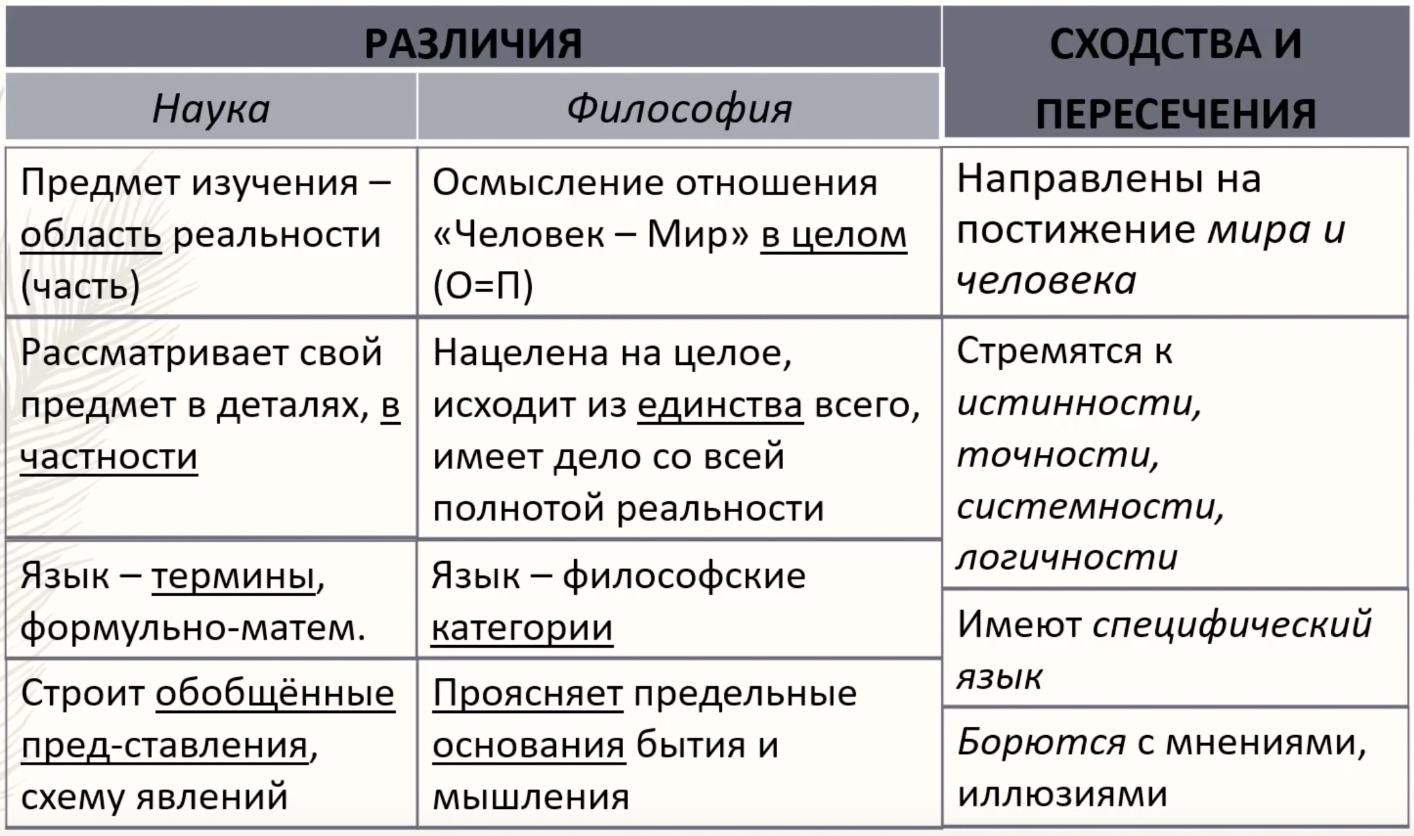
\includegraphics[width=0.8\linewidth]{pictures/sciphil.png}
    \label{sciphil}
\end{figure}

% Каждая наука выделяет в качестве предмета изучения определенную область реальности.
% Философия же занимается осмыслением отношения человек-мир в целом.  Сходство в том, что объект у этих видов культуры один --- действительность или то, что есть. 

% Философия нацелена на целое,
% в которое к тому же не только мир включается, но и мы сами во всей полноте и
% парадоксальности с плохим и хорошим и мира и нас. Поэтому объектом философии,
% который совпадает с предметом, является прежде всего отношение человек-мир в
% целом. 

% И различные философские концепции, а также настроенные в их свете
% умонастроения людей в различные культурно-исторические эпохи базируются именно
% на различном осмыслении этого отношения. Многие же, поскольку нацеливаются на
% формирование знания, вынуждены в свете этого целостного настроения вдаваться в
% подробности, детали, частности, то есть из всего в целом выделять для своего
% изучения предметы. Так в отличие от философии, представляющие в нас возможность
% и необходимость иметь дело с целым, каждая частная наука имеет в качестве
% предмета своего изучения какой-то кусочек реальности, какую-то часть целостного
% отношения человек-мир. Лингвистика язык, биология живую природу, химия состава
% превращения веществ, социология, человеческое общество и так далее. Наука по
% сравнению с философией избирает путь части, в том числе разбора на части,
% представления своего предмета как части реальности не в целостной слитости со
% всем остальным, а в его выделенности в частности. Несмотря на такие различия в
% нацеленности и философии и наука стремятся к истинности, точности, системности,
% логичности. Хотя требования, например, истинности суждения ученого-философа
% может пониматься несколько по-разному, невозможно себе представить, чтобы
% философские поиски и научные исследования ввели стремление к ложности. Здесь
% истина объединяет скорее даже не как эпистемологическая категория, но как
% этическая, поскольку выбор истины в противоположность лжи, прежде всего выбор в
% ту сторону, что мы считаем благом. Для своих различных задач, философии, как
% имение дела с целым, и науки, как познание аспектов реальности в частности, у
% данных видов человеческой деятельности, безусловно, имеются различные способы
% подхода к своим задачам и их решениям. Несмотря на то, что мыслительные операции
% мы производим как в науке, так и в философии одинаково, постановка, проблема,
% анализ, синтез, сопоставление, выделение общего и особенного, систематизация,
% формулирование выводов и так далее. Язык науки и философии различаются
% достаточно сильно. Каковы же языковые инструменты, используемые для выражения
% научной мысли, в отличие от философска. Этого мы касались в первом вопросе
% предыдущей темы, когда говорили о коммуникативных аспектах науки. Основы
% научного языка составляют особые понятия, которые называют терминами. Примеры мы
% тоже приводили, но давайте из разных наук еще повспоминаем вектор, рецептор,
% электроли, социальная группа, девиантное поведение, себестоимость, литерация и
% так далее. Помимо отсутствия в них экспрессивности, эмоционально ценностной
% окраски, первое, что также бросается в глаза, это точность терминов и
% стремящаяся к максимальной однозначности референтность, то есть строгое
% соответствие слова, словосочетания, наблюдаемому в реальности или так
% называемому идеализированному объекту, которым пользуется абстрактное научное
% мышление, например, материальная точка, абсолютно черное тело и так далее. В
% отличие от терминов в научном языке для философского основу составляют категории
% добро, красота, истина, свойства, структура, части целого, количество, качество,
% закон, уникальное, универсальное и многие подобные слова составляют несметный
% список философских понятий. Почему? Их нельзя поставить в один ряд с научными
% терминами. сделать это невозможно, как раз потому, что эти слова не имеют
% определенной референции в реальности, но задают сами условия нашей понимающей и
% исследующей работы с реальностью. Имеется в виду не то, что, не знаю, девиантное
% поведение, например, реально наблюдается, а красота или часть, нет. Речь о том,
% что у прекрасного и безобразного части и целого движения и покоя и так далее
% может быть совершенно различное смысловое наполнение, различное ценностное и
% этическое окрашивание в зависимости от тех мировоззренческих оснований в свете,
% которых мы называем нечто прекрасное, сопоставляем части целое, определяем в
% качестве движения или покоя. А, например, катет прямоугольного треугольника
% остается термином для его стороны, прилегающий к прямому углу со времен
% древнейших геометров и на протяжении истории науки свое значение не меняет. Мы к
% этому вернемся с вами сегодня в следующем вопросе и на примере категории части и
% целого рассмотрим, как их смысл различается в разные эпохи в зависимости от
% философских оснований каждой культурно-исторической локальности. Что же касается
% в этом плане сходств, несмотря на то, что в языковом плане наука и философия
% используют различные средства, объединяет их факт выражения своей мысли на
% особом языке, отличном от обыденного. Хотя философия во многом ближе к обыденной
% речи, чем наука, и всматриваться в естественный язык как в отражении оснований
% человеческого миропонимания, все же она с предельной строгостью говорит на языке
% понятий, которые в обыденной речи лишь интуитивно подразумеваются. Точнее, было
% бы сказать, что философия в этом плане имеет специальную цель разворачивание
% предельных смыслов понятий, в то время как обыденный язык их интуитивно как бы в
% свернутом, нераспакованном виде использует для цели коммуникации. И вот отличие
% языка науки от повседневного естественного языка еще более очевидно. На огромную
% долю наука в ее стремлении к установлению функциональных связей приходит в
% область искусственного языка, это прежде всего язык математики. Безусловно,
% обыденный язык, особенно в современности, в многом, благодаря СМИ, выхватывает
% научную лексику, вовлекая ее в коммуникацию. Однако, как и в случае с
% использованием философских понятий, от него не стоит ожидать строгого
% соответствия терминов их научным значением и глубокого четкого понимания сути
% явлений, так привлекательно умно названных наукой. И еще один пункт в нашей
% табличке давайте отметим, что мы имели в виду, когда определяли науку как теорию
% действительного. Тут предполагается ответ на два вопроса. с чем и как наука
% имеет дело, когда формируют знания. Наука имеет дело с предметами реальности. С
% беспредметностью наука не работает. Однако, то, что может в той или иной
% ситуации быть для человека совершенно не в предметном статусе, наука также
% способна делать предметы. Например, ощущение для художника, который его
% разворачивает в своей смыслополагающей деятельности, совершенно не то же самое
% ощущение, которое у этого художника наблюдает психолог. Для исследователя это
% предмет изучения, предмет психической реальности. А для художника этот один тот
% же феномен имеет значение не в качестве предмета, а в состоянии переживания, в
% котором он творит, и ему дела нет до того диагноза, который ставит ему психолог.
% И второй момент в нашем суждении то, что нереально науку не занимает. Даже
% виртуальная реальность, которой, на первый взгляд, в мире нет, на самом деле в
% какой-то мере реальность имеет место в нашей действительности и, надо сказать,
% немало на нашу актуальную реальность влияет. Поэтому к ней у науки информатики,
% кибернетики, психологии, социологии, математического моделирования и так далее
% проявляется не меньше интерес, чем, например, к природной действительности. А
% вот единорогам и русалкам ученые в реальности отказывают, поэтому, если ими и
% занимаются, то только как предметами фольклора или эстетическими образами
% филологии и науках об искусстве. Следующий вопрос, как наука со своими
% предметами имеет дело? Она их представляет, ставит перед собой. Как можно
% предмет научного исследования поставить перед собой? Не говоря уже о зрительно
% ненаблюдаемых для психолога феноменах психики или взаимодействующих молекулок у
% химика, даже медик, перед которым стоит человек, пациент, не может физически
% поставить перед собой человека вообще. Да, исследует тело он сейчас у
% конкретного человека, а у химика сейчас в колбе идет конкретная реакция. Но
% конкретными вещами ученые могут заниматься только в свете представления о
% человеческом теле вообще, о психике вообще, о химической реакции вообще. Наука
% не в первую очередь имеет дело с уникальным. На самом деле, каждый раз
% уникальным человеческим телом, психикой, животным, веществом и так далее. А с
% уникальным только как вариация воплощения универсального. Причем универсальное,
% общее, сходное, почему-то для науки важнее. Единичного, уникального,
% индивидуального. Между тем, как каждая конкретная вещь явилась ученому и самим
% исследователям, всегда прочерчивается экран обобщенного теоретического
% представления, которое абстрагирует или выделяет в уникальное, универсальное
% посредством наложения на уникальную, мыслимой, универсальной форму. Что же
% философия? Ее цель не составление знания о действительности, а прояснение
% предельных оснований бытия и мышления. И тофтологически, философия сама себе и
% цель и средство. Например, известнейший мыслитель XX века Мартин Хайдегер дает в
% своих лекциях такое определение «философия есть философствование». То есть,
% философия занимается осмыслением, пониманием, смысла всего в целом и продуктом.
% Такой деятельностью может быть только тоже мысль, понимание. Никакой другой цели
% у философии нет. Нет и никакого другого продукта. Это осмысление ради
% осмысления, собственно, человеческая деятельность. И если вам говорят, что
% философия имеет цель на первый взгляд нечто иное, например, научить чему-то или
% что-то воспитать, то имеется в виду научить мыслить или воспитать культуру
% мысли, но вовсе не научить жить, не научить какому-то мировоззрению, не научить
% мудрости. То есть, еще раз, главная задача философии не выдать какую-то
% информацию, а разработать и дать человеку инструменты осмысления, побудить его
% задаваться собственными вопросами и искать истину. Что же, в науке разве ученые
% не этим занимаются? В том-то и дело, как исследователи мы тоже осмысляем, но в
% рамках профессиональной деятельности ученого мы берем эти инструменты и в свете
% истины что-то видим, изучаем в своих объектах. А как философы мы как бы
% оглядываемся на то, благодаря чему есть то, что перед нами, на сам свет истины,
% который как бы у нас за спиной, когда мы познаем. Мы рефлексируем свою
% деятельность и даже если по профессии занимаемся наукой, это не значит, что в
% нас, как в живых человеческих существах, не присутствуют философские способности
% к видению мира в целом, постановки под вопрос даже устоявшегося знания и
% пониманию первопричин происходящего. Так вот, общее. Для философии науки мы
% уловили, должен рождаться смысл, должна присутствовать истина. Не только
% философия в своей, смыслопорождающей деятельности, борется с мнениями и
% иллюзиями. Науке не в меньшей степени приходится совершать усилия отделения
% научного знания от уже научного типа снежного человека, инопланетян,
% рептилоидов, экстрасенсов и так далее. Понятно, да? И объяснять в своих строгих
% формулировках научные законы в противоположность расхожим обыденным их
% трактовкам и неточным интерпретациям. Вы это, как ученые, прекрасно знаете по
% себе. Например, если мы скажем, что электроны вокруг ядра атома движутся по
% орбитам разной формы, сферическая, гантелеобразная или сложная в виде цветочка,
% химик или физик элементарных частиц нас поспешит поправить. Электроны, нельзя
% сказать, движутся вокруг ядра, тем более, конечно, не представляют собой эти
% орбиты. Объемные рисуночки, сферические, гантелеобразные, это условное
% изображение плотности вероятности наиболее вероятного пространства, опять же, в
% кавычках, нахождения электрона в том или ином энергетическом состоянии вблизи
% ядра. Не точка в пространстве с определенными координатами, а одновременно и
% волна, он как бы размазан по этой вероятной области. И вообще, давайте я вам
% покажу, откуда это все берется, обратимся к решению уравнения Шрюдингера для
% волновой функции. И понеслось. Ученые обязаны нас поправлять, возвращать из
% размытости обыденного представления на рельсы научного знания, иначе мы
% ориентироваться в мире будем по мнениям, то есть по мнимости, а не по точному,
% теоретическому. Философы по-своему борются против мнения, расхожих представлений
% и стереотипов. С их точки зрения, не специалисту простительно, например, иметь
% смутные представления об элементарных частицах, но непростительно, скажем, не
% рефлексировать навязываемые со стороны стереотипы о выборе профессии или о том,
% должно ли счастье быть общепринято. Но, в принципе, совершается сходное движение
% через объяснение, показывание ложности и губительности для нас таких
% недопроясненностей, готовых схем, удобных решений. 



\subsubsection{Наука и религия}

\begin{figure}[H]
    \centering
    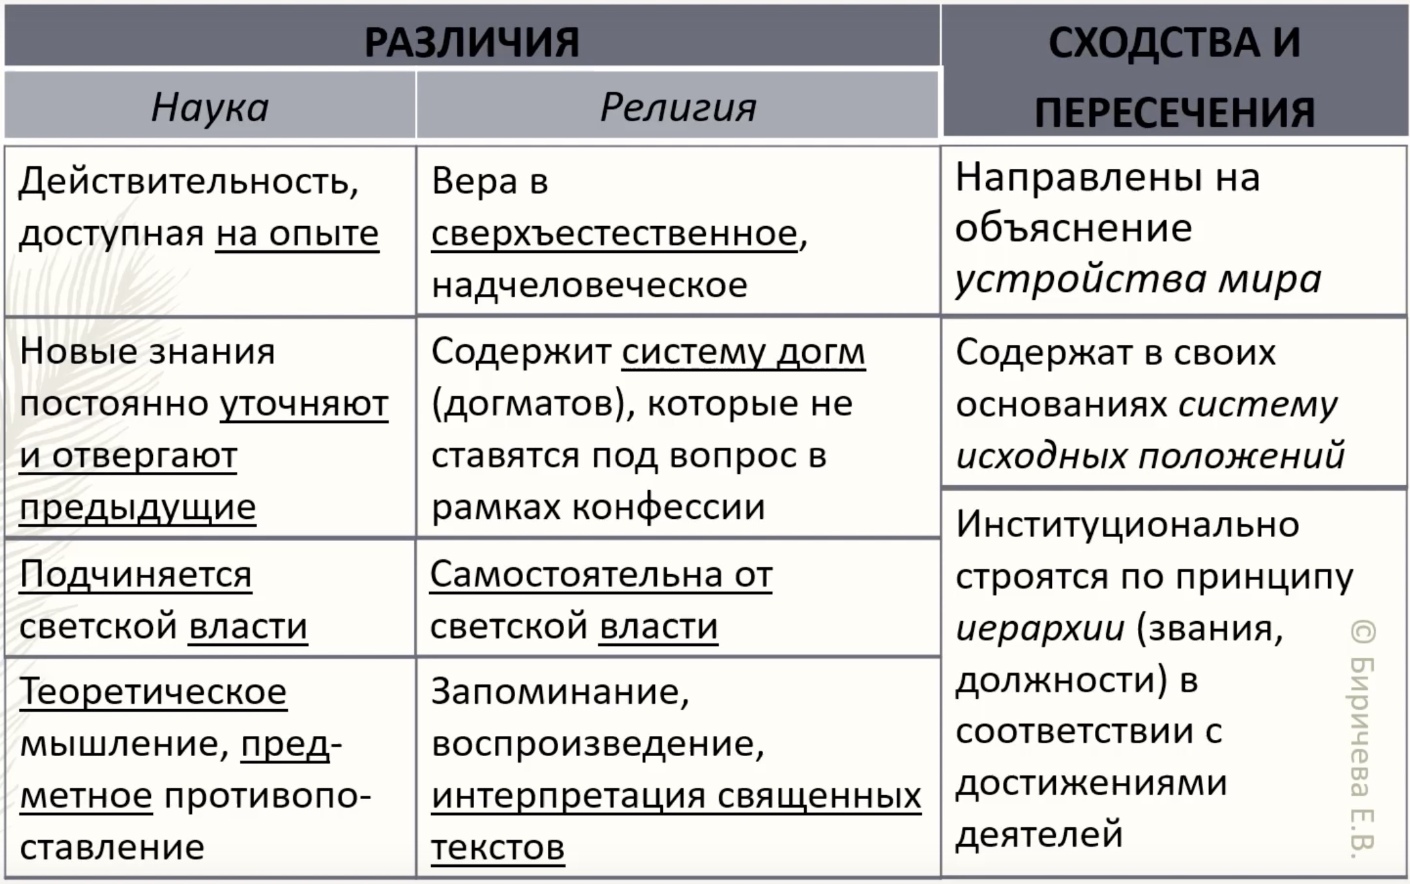
\includegraphics[width=0.8\linewidth]{pictures/scirel.png}
    \label{scirel}
\end{figure}

%  Прежде всего, отметим,
% что наука изучает объекты и явления действительности, которые доступны на опыте.
% Религия же основана на вере в сверхъестественное и трансцендентное, то есть
% антелеком посвящена незримым, высшим основаниям всего. А наука, как мы только
% что проговорили, сопоставляет с философией, имеет дело только с тем, что дно,
% что мы можем реально в мире встретить. Но, безусловно, оба эти вида культуры
% каждый по-своему объясняют первоосновы мира и трактуют как-то специфику
% человека, как внутримирного существа. Тут бегло заметим, чем религия отличается,
% в том числе, от мифологии, чтобы вы не путали. В мифе, конечно, есть
% представление о сверхъестественных силах, но, помимо этого, там намешаны и
% элементы других феноменов культуры, повествования о богах и героях, как
% эпические, литературные произведения, какие-то рецептурные рекомендации по
% поводу обустройства быта, философские концепции, так или иначе, трактующие
% благо, справедливость, природу, материя, способ возникновения мира, в жизни
% человека. Ну, понятно, да? Любая религиозная система концентрируется только на
% представлении надмирового, надчеловеческого, божественного, причем не
% обязательно бог один, не обязательно это сверхъестественное персонифицируется и
% не обязательно, кстати, божество вне мира мыслиться, то есть индуизм, даосизм,
% синтоизм и многие другие системы это тоже религии, а не мифологии, хотя, еще
% раз, может не быть антропоморфного божества, их может быть много и они могут
% мыслиться присутствующими в мире, а не вне его. Естественно, из этих
% представлений можно логически выводить какие-то этические рекомендации, советы
% по устройству быта, но это уже будут богословские, научные или философские
% интерпретации. Чего? Это второе главное отличие от мифологии священных текстов,
% которые содержат догмы или догматы, нерушимые и неотменимые в рамках
% соответствующей системы основоположения. Миф текуч, в нем возможны в самом
% разнообразные добавления, искажения, интерпретации при передаче из уст в уста.
% Любая конфессия фиксирует, свои базовые положения закрепляют священных текстов.
% И очень много усилий надо приложить, чтобы какой-то новый догмат ввести в эту
% систему. С огромным трудом подобное, например, удалось сделать в православии в
% XIV веке Григорию Паламе. Он предложил в противоположность католическому учению
% разделять понятия энергии и сущности в отношении Бога и его деяний. А вот
% скажем, такой шаг в сторону сближения с исламом, как иконоборчество, в
% православии в свое время потерпел неудачу. Вокруг этих ожесточенных споров
% творились поворотные исторические события, заключались под стражу и гибли люди.
% Так что религия четко держится своих догматов и немногочисленные случаи их
% изменения скорее исключения, чем правила. В отличие от этого, наука развивается
% путем постановки под вопрос действующих знаний и производства новых, уточняющих
% или преодолевающих предыдущие. Со второй темы можно здесь вспомнить
% постпозитивистов Карла Поппера и Тома Сакуна, которые по-разному предлагают
% рассматривать развитие науки эволюционно или путем научных революций. Но
% сходятся они в том, что все-таки со временем одни научные теории и подходы
% заменяются другими. Тем не менее, нельзя отрицать, что как наука, так и религия
% в любом случае содержат в своем основании систему исходных положений. Просто
% внуки они периодически пересматриваются, а в религии если пересматриваются, то
% возникает новая конфессия отдельно на своих основаниях и становится
% равноправными другими. Так, когда-то единое христианство разделилось на
% православие и католицизм, а затем от последнего отмежевался протестантизм в
% различных вариантах лютеранства, кальвинизма, англиканства и так далее. Об этом
% в темах о средневековье и возрождении вам подробно расскажет Светлана
% Викторовна. Какие еще отличия можно выделить? Обычно религия в современном мире
% существует автономно от власти, то есть давайте применять разобранные в
% предыдущей теме термины, институция анализируется в качестве самостоятельной по
% отношению к светской власти системы. А вот наука чаще всего входит в эту
% систему, подчиняется. Например, мы с вами на прошлой теме говорили, что
% Министерство науки и высшего образования РЭП занимается управлением и сельской
% деятельностью. Что касается в этом отношении сходств, институты науки и религии
% строятся по принципу иерархии должностей, званий, рангов, служителей или
% сотрудников в соответствии с достижениями каждого деятеля. То есть
% институционально предполагаются как в научном, так и в религиозном сообществах
% системы соподчинения и иерархического расположения в зависимости от тех или иных
% показателей, которые к тому же оцениваются специальными внутренними инстанциями.
% Наконец, в плане когнитивной специфики исследовательская работа предполагает
% теоретическое мышление, представляющее предметы в качестве противопоставленных
% знаний ученого. В религиозных практиках распространены в первую очередь
% запоминания, передача основ учения через религиозное обучение и интерпретация
% священных и авторитетных текстов. Также неотъемлемой составляющей являются
% строго регламентированные ритуалы, обряды, священодействия. В науке аналогом
% можно называть, пожалуй, соблюдение металлогических процедур, однако ввиду того,
% что они сами трансформируются, меняются, уточняются, изобретаются новые и так
% далее. Не факт, что это пойдет в рубрику сходства. Вообще наука и религия в
% современном мире достаточно полярные позиции, занимают по отношению друг к другу
% и трудно выделить много пересечений для них, глаза бросают скорее различия. Но
% думаю, того, что мы тут отметили, достаточно для представления экзаменей.

\subsubsection{Наука и искусство}

\begin{figure}[H]
    \centering
    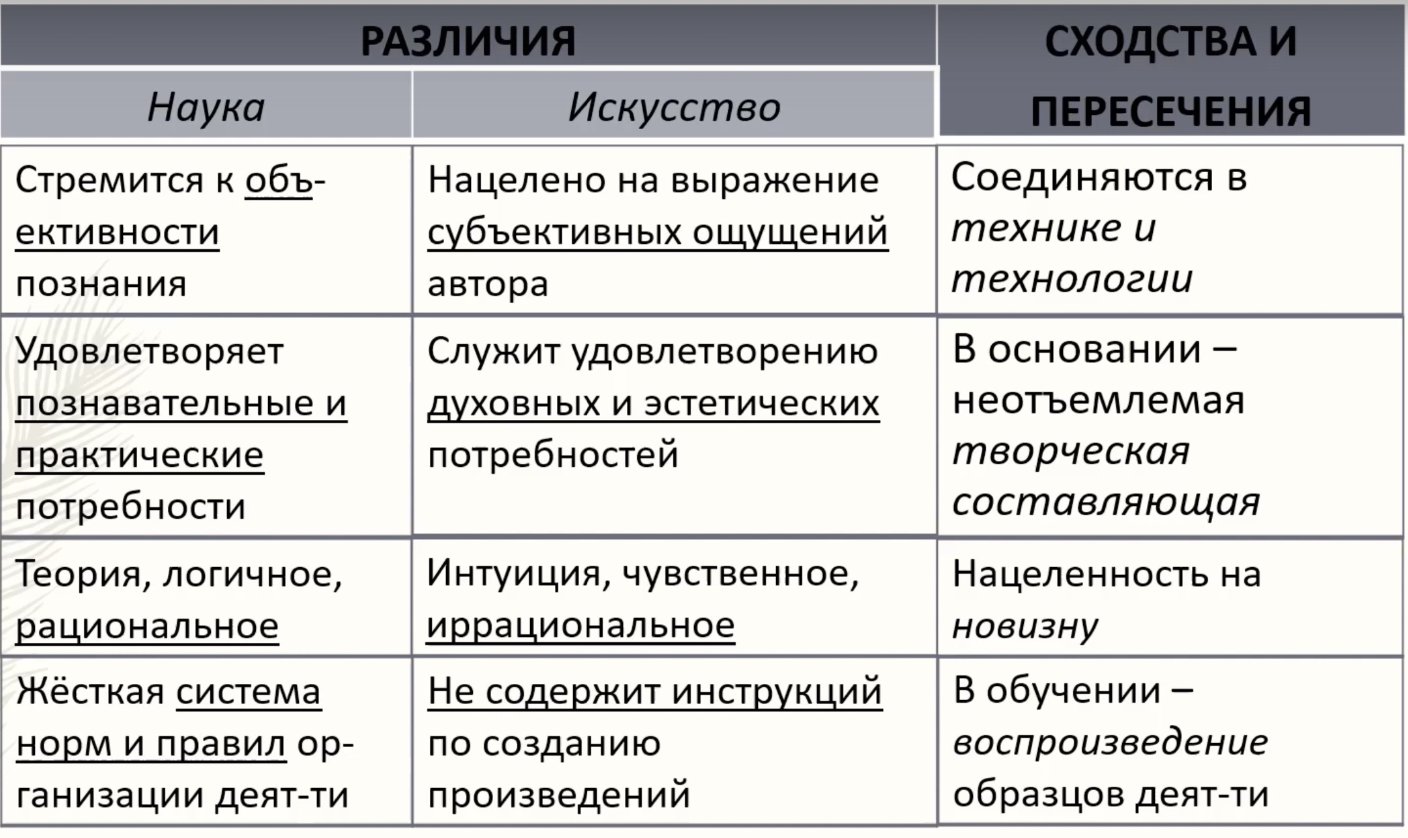
\includegraphics[width=0.8\linewidth]{pictures/sciart.png}
    \label{sciart}
\end{figure}

% поэтому перейдем к последнем сравнению, наука и искусство, чем у нас различаются
% и в чем сходятся. Тоже достаточно неблизкими друг другу кажутся эти виды
% культуры. Первое отличие, которое сразу приходит на ум, заключается в том, что
% наука стремится к объективности выражаемого знания. Тут объективность можно в
% двух смыслах брать, как отражение реальности самой по себе, представление его
% обобщенных законов и как противоположное субъективному, личному, то есть не то,
% что одному и не виду показалось, а что разделяется большинством в плане
% интерсубъективности. Искусство же не особо интересуется универсальными
% закономерностями и достоверным их описанием, а нацеливается на выражение
% субъективных переживаний и ощущений автора, его уникальной точки зрения, его
% новаторского способа видеть, пусть и ту же самую реальность. Пересекаются наука
% и искусство в технике и технологии. Это мы уже отметили, выше говоря, о
% древнегреческом слове техно, которое означает искусство в широком смысле как
% специфическая человеческая деятельность, направленная на создание того, что не
% рождается и не живет само по себе, но требует нашего осмысляющего участия. В то
% время, как наука направлено на удовлетворение мировоззренческих, познавательных
% и практических потребностей, искусство служит удовлетворению духовных и
% эстетических потребностей человека. Но и там, и там лежит в основании
% неотъемлемая творческая составляющая. Иногда кажется, что искусство это наиболее
% творческая деятельность, но на самом деле, во-первых, в искусстве огромную долю
% занимают те же самые коммуникации и рутинная работа, как и в науке, когда надо
% отточить мастерство, тренироваться, набить руку, много чего прочитать, обсудить
% с коллегами и так далее. А во-вторых, исследователь не менее творец, чем
% художник, просто он создает новое знание или техническое изобретение, а не
% картину или образ, скажем, спектакля. То есть, креативные способности можно в
% любой деятельности равно проявлять. При этом в науке мы опираемся на
% рациональные, логические, теоретические способности, а в искусстве большее
% значение имеет опора на интуитивные, чувственные и рациональные способности
% человека. Но, конечно, как и любая творческая деятельность наука и искусство,
% каждая по-своему нацелена на новизну. Наконец, можно такие еще различия
% предположить. Если наука имеет систему норм и правил ведения научного
% исследования, строгий язык, логику и так далее, то искусство не содержит
% однозначных инструкций по созданию произведений. Тем не менее, в обоих случаях
% обучение предполагает изучивание техник работы и задания на их практическое
% применение воспроизводства созданного ранее. Как, например, химику надо
% проделать множество лабораторных работ, воспроизводящих уже известные синтезы,
% аналитические процедуры и технологические процессы. Так и, скажем, скульптор
% сначала обучается слепить череп, вырезать барельеф, нагончарить кружку, а потом
% уже придумывает свой абсолютно новый шедевр. И далее, по подобной схеме вы
% самостоятельно на основе своих эрудиций и жизненного опыта сможете сопоставить
% науку с чем угодно, потренируйтесь на семинаре, это сделать по поводу
% образования, морали, политики и других феноменов культуры. 

\section[Культурно-исторический контекст развития науки и его философские основания]{Культурно-исторический контекст развития науки и его философские основания
(онтологические, гносеологические, этико-аксиологические)}

\subsection{!!! Понятие культуры в связи с её фундаментальными основаниями}

Культурология
знает, ведает, безусловно, чрезвычайно много о культурах, но сколько я не читала
труды исследователей в этой области, находила только поверхностные определения
культуры, не в смысле плохие, но замечающие только внешние проявления, все то,
что у нас обычно и ассоциируется с культурой, традицией и ценностями. Это все
замечательно. 

Однако, такое знание, хотя, несомненно, важно, интересно и для
определенных целей полезное, ничего не говорит о том, почему сложилась именно
такая культура, почему не другая, почему не иначе. Говорить, что так исторически
сложилось, или потому, что такой менталитет, или благодаря такому особому языку,
значит, повисать над бездной.
Мы всегда можем дальше спросить, а почему так
сложилось, почему такой язык и менталитет, на каком основании? 

Это только
философия может помочь, поскольку именно она занимается прояснением предельных
оснований человеческого бытия и мышления. И, по сути, понимание особости каждой
культуры делая ответы на тот же философский вопрос о своем собственном, которым
мы задавались на предыдущей теме, говоря об индивидуальном в человеке. 

Культуры отличаются своими традициями, идеалами, нормами, ценностями,
которые, в свою очередь, выросли из своего собственного, каждой культуры. Они
сформировались в свете определенного способа бытия, образа организации жизни.
Что значит способ бытия? это образ мысли, способ видения мира и себя в нем,
способ понимания окружающей действительности, в русле которого мы выстраиваем
свои отношения с миром, с природой, с другими людьми, с теми же продуктами,
имеющиеся культурой, в которой рождаемся. 
Поэтому мы и говорим, что философское
определение культуры это способ бытия, а именно в случае человеческой культуры
способ понимания человека мира и своего положения в нем, в свете которого
выстраивается определенное отношение к окружающей действительности,
результирующиеся в выработке норм и идеалов человеческой деятельности. 

Когда я
говорю об основаниях, как о способе бытия, я имею в виду, что оснований нет в
виде какого-то определенного что. Мы знаем, что исторически меняются содержание
научного знания, нормы и идеалы в искусстве появляются и уходят со сцены
религиозной системы и так далее. Надежное основание возможно только не
субстанциально в форме как образа действия или способа бытия. Конечно, плюрализм
или множественность оснований и в форме как, очевидно, в случае каждого
человека, но надежен для меня только мой способ бытия, другой не может быть за
меня моим способом, хотя с содержаниями мы можем с одинаковыми иметь дело.

Способ как конкретный путь, образ действий, по определению единичен, целостен и
уникален, то есть своей особостью и будет отличаться от других способов, но он
не зависит от того, на материале каких содержаний действует, он как-то поступает
со всем, что ему дано, что-то видит, что-то игнорирует, что-то использует, что-
то нет и так далее. На основании чего мы что-то делаем, видим, используем. Не
потому, что так принято или все вокруг считают это ценным. Мы можем поставить
это под вопрос и заменить одни говорят одно, другие другое, третье, третье. Кому
поверить? Почему надо вот это делать, не вот это? Что реально, а что иллюзорно?
Почему я к этому так отношусь? На подобные вопросы мы даем каждый пропускать
через себя, думавая по-своему, на материале, личностной истории и в свете своих
уникальных склонностей, способностей, наполняя смыслом, даем свои ответы. 

Мы
отталкиваемся от своего фундаментального основания, которое неизменное, а не
имеющимся из стороны в сторону, гонимые то одним, то другим чем-то мнением и не
слепо автоматически делаем, как принято. Иначе бы основания не переосмыслялись и
эпохи бы не менялись, и культура была бы у людей одна одинаковая по всему
земному шару. 

И вот точно так же, рефлексируя по направлению к основанию
культуры, мы приходим к необходимости прояснить самые фундаментальные из них,
то, в связи с чего мы мыслим и поступаем в бытии, речь об онтологических
основаниях, в контексте которых также возможным становится прояснение и других
философских оснований, гносеологических, этических, аксиологических и так
далее. Тогда, парадоксальным образом, философия у нас становится философией и
культурой, ведь именно прояснением этих оснований, понимания всего в целом, а у
разных культур они разные, мы занимаемся.

\begin{figure}[H]
    \centering
    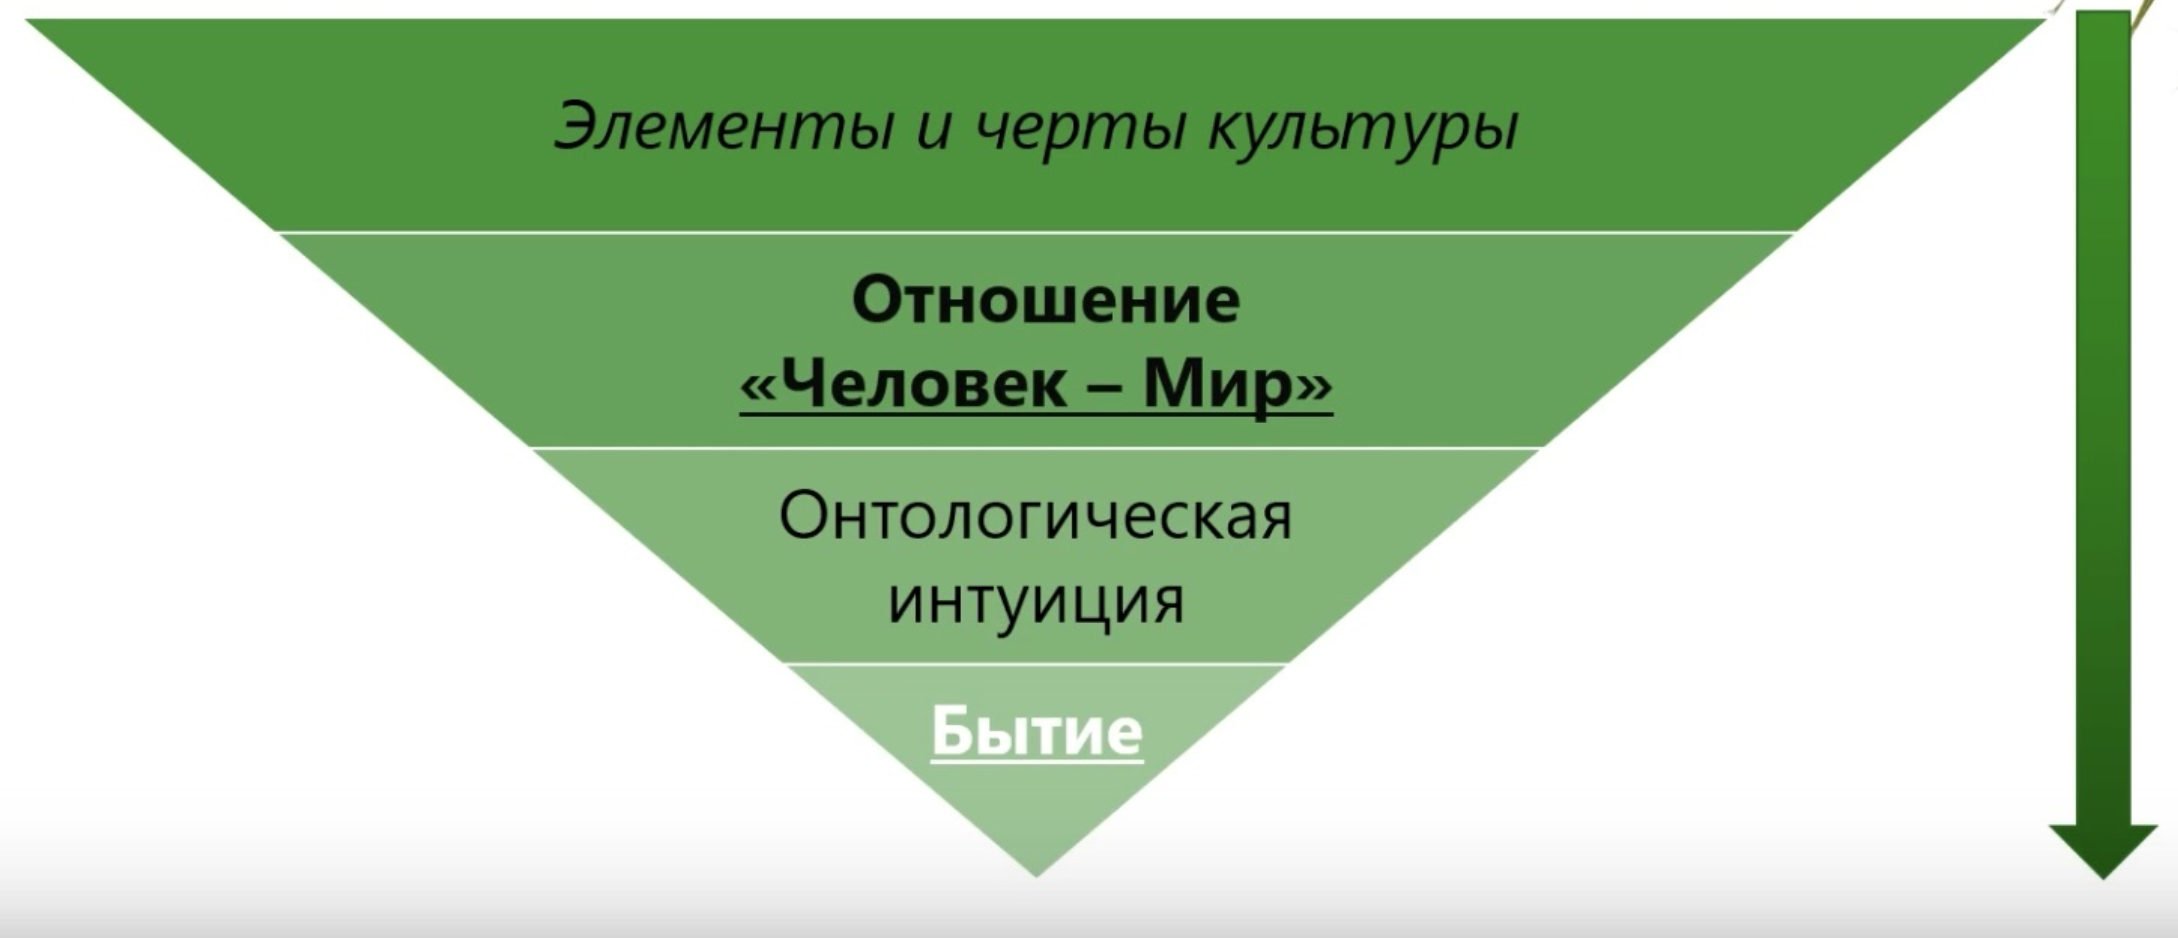
\includegraphics[width=0.8\linewidth]{pictures/hz.png}
    \label{hz}
\end{figure}

% В ротивоположность чему выстраивается способ бытия? причем каждый
% раз различный в исторической перспективе у представителей разных современных
% культур, в пределе у каждого человека.
% Бытие противоположно
% небытию и способ быть выстраивается вопреки или в ответ на страх небыть. То есть
% в основании нашего бытия предельным образом лежит на самом деле небытие,
% которого мы боимся, поскольку знаем о своей конечности и отталкиваясь от угрозы
% небытия стремимся быть максимально добротно быть, достигать пункты своего
% существования. Эту идею, причем применительно к осмыслению культурно-
% исторических трансформаций мировоззрения, проводит в своей книге «Муж что быть»
% выдающая немецкий мыслитель Пауль Тилли. тревога небытия постигается нами в
% глубоком детстве, обычно в возрасте от 3 до 5 лет, когда мы начинаем осознавать
% свою конечность во времени и пространстве. В пространстве мы познаем границы
% своего тела и то, что не можем по своему желанию непосредственно оборудовать
% другими людьми и внешними обстоятельствами. Безусловно, временность нашего
% существования каждым переживается как просто страх смерти. Однако, даже в языке
% есть такое выражение «Может быть что-то страшнее смерти». И вот для каждого
% человека в той совокупности окружающих его условий, в которой формируется его
% личность, то, что страшнее смерти, переживается уникальным образом и
% сворачивается с глубокого детства интуитивно в ту или иную форму угрозы небытия,
% чего, как вы думаете, можно бояться сильнее смерти. Например, хаоса и
% неупорядоченности, бессмысленности своего существования и окружающего мира,
% тотальной необеспеченности человеческого положения, возможности не оправдать
% ожидания окружающих людей, поступить не по совести, отказаться отделенным от
% всех, одиноким и так далее. Противоположность каждый раз конкретной форме угрозы
% небытия каждый человек выстраивает свой способ быть. Например, опасаясь хаоса,
% человек будет упорядочивать и рационализировать, структурировать и
% систематизировать все вокруг. Страх и необеспеченности логично развивать
% медицину и экономику, стараясь использовать природу на службу человека,
% удовлетворяя потребности и пытаясь продлить жизнь. Если человек боится не
% оправдать ожидания других людей, то посвятить себя благородному делу, вежливо и
% учтиво со всеми будет обходиться, учитывать интересы и особенности других людей,
% стараться соответствовать тем месту и роли, которые за ним закрепляются в
% социальной структуре и так далее. Тут, когда мы говорим о культуре, надо не
% забывать как раз о том, что культура как такой способ бытия не определяется
% географическими или национальными границами. Безусловно, языковая, социальная
% среда, историческая память, экономико-политическая ситуация связывают общность
% условий. Однако, это не детерминирует нас полностью, и мы можем принадлежать
% разным типам культур с ближайшим соседом, но почувствовать родство с человеком с
% другой половиной земного шара. Бредом, конечно, далеко не все люди осознают
% собственную тревогу небытия, да и кризисные моменты нашей жизни могут
% существенно повлиять на смену типа фундаментальной тревоги. В этом случае нам
% придется кардинально пересмотреть основания своих поступков, скорректировать
% характер, разменить жизненные цели и ценности. в графических регионах можно
% говорить лишь о преобладающем типе культуры. Наконец, последний момент,
% наверное, вы почувствовали культуру тревоги, хаоса и неупорядоченности, та, что
% исторически выросла на западноевропейской почве. Именно ее традицию внуки и
% философию мы, собственно, должны разбирать в нашем курсе. С ней заодно очень
% близко идет культура тревоги необеспеченности, как мне кажется, навязываемая
% сейчас ему миру со стороны США. В рамках глобализации сегодня мы, в смысле
% представители остальных культур, испытываем на себе влияние и, я бы даже
% сказала, давление со стороны этих двух типов культур, действующих совместно в
% плане стандартизации и универсализации, в том числе в сфере науки, в плане
% экономического расхода всего на планете, мечтания определения жизни, бессмертия,
% комфортного существования и подобных вещах. Это неплохо и нехорошо, просто важно
% понимать, откуда у современной науки ноги растут. Но важно не забывать, что в
% мире есть еще множество типов культур, в том числе наша тоже особенная. И нет,
% на ни хуже, ни лучше другой. Мы равноправны, поскольку каждый чувствует в той
% или иной форме экзистенциальную тревогу небытия и каким-то образом ей конкретно
% отвечают в своей ситуации, своим способом. способы не лучше и не хуже друг
% друга, потому что просто-напросто каждый хорош в отвечании на свою угрозу
% небытия и, понятное дело, плох, если им пытаться отвечать другому
% фундаментальному страху. В частности, поэтому на отечественной почве, как вы
% сплошь рядом видите, не проживаются решения, может быть, полезной и
% рациональной, но органично выросшей на почве иных культур. Таким образом, теперь
% мы в данной теме о культуре сможем заложить для себя фундамент понимания
% существа культурно-исторических эпох. Для этого опишем в логике культуры как
% способа бытия методологию, с помощью которой мы будем двигаться в темах
% следующего раздела, который называется «История науки в ее связи с философией»,
% начиная изучение каждого типа науки с прояснения его культурно-исторических
% условий и философских оснований соответствующей эпохи. Здесь также необходимо
% кратко привести конкретные примеры, какими были основания культурно-исторических
% эпох, которые нам предстоит изучать, чтобы стало хоть немного понятнее, как
% различное содержательное наполнение, ну, какое, да, наполнение могут получить
% основания и в соответствии с ними тип науки. Итак, антологические, сущностные и
% бытийные основания. Это фундамент определенного типа мышления, добираясь до
% которого сквозь все внешние наслоения, ну, там, традиции, социально-политические
% условия, ценностные ориентиры, мы как раз получаем ключ к пониманию оснований
% мышления, неважно, конкретного человека или культурно-исторической эпохи. Хотя у
% каждого из нас уникальное представление о себе, о мире и о своем месте в нем,
% если мы говорим о культурно-исторической эпохе, даже такой длительной, как,
% например, античность или средневековье, каждое существовало более тысячи лет, то
% имеют место тенденции примерно одинакового понимания этих базовых моментов всеми
% членами данного общества, сформировавшись в определенный момент, целостные
% представления о мире и человеке безусловно отражаются в языке соответствующей
% культуры, а с языком передаются в ходе воспитания от родителей и детям, то есть
% последующим поколениям. Поэтому смена культурно-исторических эпох происходит
% медленно, для с целыми столетиями. В связи с этим, например, так сложно провести
% разделительную черту между окончанием эпохи античности и началом средних веков.
% христианское мировоззрение, легшее в основу средневекового миропонимания, начало
% формироваться как минимум за четыре столетия до того, как оно получило тотальное
% распространение в Европе, сменив собой окончательно античный тип мышления. Так
% вот, сущностные основания того или иного типа мышления как раз предполагают
% определенное понимание отношения человек-мир, которое содержательно отличается
% для каждой эпохи. Одушевленная, упорядоченная, но при этом движущаяся,
% изменяющаяся вселенная античности с отражающим ее целостность и полноту
% человеком совершенно не совпадает со средневековым иерархически сотворенным по
% замыслу Бога миром, в котором человек уже чувствует себя иначе, в частности,
% например, не имеющим права на преобразование вещей мира, на буйную творческую
% активность и праздновать развлекательный образ жизни. Что касается бытийных
% оснований, естественно, во всей эпохе далеко не все люди настолько глубоко их
% для себя осмысляют и проговаривают, чтобы дойти до самой фундаментальной основы
% своего способа мысли, до понимания категории бытия. Категория бытия, то,
% благодаря чему все есть и есть именно так, представляет собой как бы пустую
% форму, наполнение которой в рамках каждого типа мышления также происходит по-
% разному. Однако нам в ободенной жизни достаточно интуитивного ее понимания,
% которое, опять же, в ходе воспитания нами усваивается. На этом основании мы
% сами, не задумываясь об этом, строим свои суждения и из этого основания выводим
% свои представления о действительности. На этом основании действия мы поступаем
% именно определенным образом. Прояснить и проговорить эти предельные основания
% всей нашей культуры, чтобы понимать, на чем все основывается, как раз задача
% философии и философов. Они занимаются профессионально глубокой рефлексией, то
% есть вопрошением о причинах, в пределе о первых причинах всего сущего,
% устройством мира, определенным способом мыслить и так далее. На самом деле все
% люди являются стихийными философами, поскольку периодически задаются вопросами о
% причинах стихийных событий, но большинство в силу посвящения себя иным занятиям
% не практикуют рефлексию настолько глубоко до бытийных оснований, особенно для
% нас исследователей это очень полезно для того, чтобы четко для себя понимать
% основания своих научных суждений и выводов теорий. Поэтому мы обучаемся
% философии и знакомимся с помощью ее метода с историей нуки. Так вот,
% антологическим основанием является помимо понимания отношений человек мир
% интуитивное понимание бытия. Здесь под интуицией имеется в виду не шестое
% чувство, а образ мысли, складывающийся в свете того, что остается для нас
% самопонятным, безусловным, несомненным, короче говоря, тем, что не ставится под
% вопрос. Это безусловный фундамент, от которого отталкивается любая наша мысль,
% то, что далее не может быть рефлексировано. Так, забегая вперед, для современной
% нашей эпохи, пожалуй, можно условно сформулировать антологическую интуицию, как
% интуицию сложного, множественного. Согласитесь, как в личной жизни, так и в
% своих научных исследованиях мы сегодня исходим из того, что все чудовищно сложно
% и многомерно. Кучу факторов нужно учесть разными методами, а не одним тестовать
% свои образцы, проследить многогранные связи друг с другом изучаемых объектов и
% явлений. Есть такое? Другой пример. Раз мы коснулись средневековья, в средние
% века несомненным было совершенно иное факт сотворенности мира Богом. Из этого в
% любом своем действии, суждении и понимании исходил западноевропейский
% средневековый человек. Это под вопрос не ставилось, иначе бы развалилось все
% средневековое мировоззрение. Наконец, самым главным антологическим основанием
% является понимание категории бытия в рамках данного мировоззрения. Понять
% антологическое существо эпохи определенного типа мышления означает понять ответ
% на вопрос, что значит быть для этой эпохи или в рамках этого мышления. Пример
% про средневековье быть значит быть сотворенным, быть на своем месте в
% соответствии с божественным замыслом. Тогда как для нас сегодняшних рискну
% предположить, быть означает нечто иное. Скорее всего в своей массе мы понимаем
% бытие как изменчивое, текучее, разнородное. То есть для нас быть скорее значит
% быть изменяющимся, трансформирующимся, развивающимся в сложной системе
% взаимоотношений с окружающей действительностью. Здесь конечно речь идет не
% только о том, что значит быть человеком, человеком в том числе, но в
% совокупности со всем сущим. Таким образом можно наш с вами метод исследования
% культурно-исторических эпох представить в форме условной схемы. Нам сейчас эта
% схема поможет как можно двигаться к антологическим основаниям культурно-
% исторической эпохи, чтобы понять ее существо. в начале стоит набросать контекст,
% разбираясь с действительными чертами и особенностями исследуемой культуры, то
% есть погрузиться во внешнюю специфику эпохи, в процесс чего можно будет
% прослеживать связи и закономерности развития этих особенных черт. Как при первом
% знакомстве с человеком, мы сначала воспринимаем его внешний вид, как он говорит
% и о чем, в какой манере, какие черты характера проявляет. На данном этапе
% знакомства с той иной культурой мы будем характеризовать как раз традиции и
% ценности в искусстве, в политическом устройстве, в быту и повседневной жизни
% людей, в социальных условиях человеческого бытия соответствующего периода. Более
% глубокая рефлексия далее выведет к антологическим основаниям эпохи, скрытым на
% глаз при поверхностном знакомстве, позволяя прояснить основную суть
% мировоззрения. Также с людьми, с кем мы начинаем понимать, почему человек именно
% так поступает в той или иной ситуации, почему у него сложился такой характер и
% на основании каких мировоззренческих принципов он высказывает те или иные
% суждения. То есть для культуры после краткого освещения контекста каждого
% исторического периода в рамках соответствующей темы, нам предстоит разобраться с
% тем, как все выделенные нами на первом этапе особенности сложились в свете
% определенного понимания отношения человек-мир. Здесь мы из принципов культуры
% будем выводить ответы на вопрос что такое мир представления данной эпохи, что
% такое человек и каким он должен быть, каковы место человека в мире. Далее мы
% сможем предельно почувствоваться в существо, рассматриваем культурно-
% исторической эпохи и постараемся улыбить антологическую интуицию, то,
% несомненно, из чего выводятся все принципы и особенности данного тип культуры.
% Наконец, мы придем к вопросу о том, что значило быть для того или иного типа
% мышления. То есть, дойдем до понимания категории бытия в том ее уникальном
% наполнении, свойственном именно конкретному варианту мировоззрения. Это, еще раз
% повторюсь, условная схема. Во-первых, можно исследовать эпоху или тип мышления
% другими способами, просто мы выбрали такой путь, позволяющий дойти до самой
% сути. Параллельно практикую усилия собственного осмысления, что тоже является
% важнейшей задачей для нашего курса. Во-вторых, конкретно эта схема нарисована в
% виде перевернутой пирамиды, однако это не значит, что бытие лежит в основании, в
% смысле какого-то квада, до которого нужно добраться. На самом деле, оно и без
% нашего исследования окружает и объемлет нас, дает нам быть, то есть не в смысле
% физического фундамента или какого-то ядра лежит у нас под ногами. Таким
% расположением слоев я хотела передать путь, которым наша мысль сможет двигаться
% по следующих темах при исследовании культурно-исторических эпох от поверхностных
% внешних особенностей к глубинной сущности. 

\subsection{!!! Система философских оснований и культурно--исторический контекст развития
науки}

Внешне система философских дисциплин может напоминать разделение науки на области знания. 
Однако разделы философии на самом деле не похожи на области исследований
в рамках науки, которые избирают каждое для себя какой-то пласт реальности и не
затрагивают другие. 

Каждая из них все равно имеет дело с отношением человек-мир, но смотрит на него сквозь призму
своих базовых категорий. Продуктивнее представить философию как кристалл, а ее различные разделы как грани. 
\begin{itemize}
    \item Онтология.
    
    Самая общая и фундаментальная грань. Онтология --- философская
    дисциплина, занимающаяся осмыслением бытийных и сущностных оснований отношения человек-мир. 
    Ее базовые категории бытие и сущие.
    
    Отсюда название греческие, то он означает то, что есть. Имеют относится
    пространство и время, качество и количество материю и идею движений, покой,
    части целой и множество других. Но все они получают свое содержательное
    наполнение в зависимости от того, как понимается бытие. 
    
    Или, если говорить
    проще, какой дается ответ на вопрос, что значит быть. Так что, говоря об
    онтологических основаниях определенной эпохи, мы сможем после прояснения самых
    фундаментальных перейти к разбору того, например, какие были представления о
    пространстве и времени или как понималась материя. 

    \item Гносеология.

    Область философии, занимающаяся вопросами познавательной
    деятельности сознания, проблемами сущности и видов знания, истинной
    достоверности сущности и методологии познания.

    То есть, гносеология тоже на все смотрит, но через призму категорий знания и познания. 

    \item Этика.
    
    Занимается пониманием блага в категориях добра, зла, долга, ответственности, греха и так
    далее. В рамках той или иной системы морали и нравственности. Базовая категория этики --- благо.

    \item Эстетика.

     Это философская дисциплина, осмысляющая сущность и формы прекрасного в художественном творчестве, в природе и в жизни. 

     Базовые категории --- красота, прекрасное.

     \item Антропология --- о человеке.
     \item Социальная философия --- об обществе и человеке как общественном существе
     \item Аксиология ---  о ценностях, идеалах и нормах.

     
\end{itemize}

% То есть, к примеру, гносиологию
% интересуют все о том, как мы познаем. Опознавать можно все, что угодно, от
% материала в руках гончара до природы блага, как такового, от букашки под ногами
% до Бога. Это все будут совершенно разные варианты познания, но все же познания.
% То же самое с эстетикой. Прекрасное, можно увидеть, услышать, ощутить во всем и
% выразить его в различных формах. Понятно, да? рамки, она высушенькая будет. Вот
% тут пример заполнения сразу. Далее. Самые фундаментальные антологические
% основания. Пропишите кратенькие ответы на вопросы. Как понимается отношение
% человек-мир, какова антологическая интуиция, то есть, что несомненно в данную
% эпоху и что значит быть или как понимается категория бытия. Мы обязательно с
% вами в таком ключе резюмируем базис античной культуры в следующей теме. У нас
% первый вопрос будет о социально-культурных условиях ее формирования. Из этого
% основополагающего ключа уже можно будет догадаться, даже если вдруг четко в
% лекции по какой-то эпохе вам это не проговорят, о ее гносеологических
% основаниях. Это какой основной источник познания, какие возникают и развиваются
% области знания, какие преобладают методы познания с этикой. Мы с вами уже
% знакомы по третьему вопросу прошлой темы. Здесь мы прежде всего спросим, что
% есть благо, как оно понимается, что такое хорошо, что такое плохо для каждой
% эпохи. Хотя это разные философские дисциплины, но вы понимаете наилучшее,
% наиглавнейшее, самое ценное моменты неразрывно связанные, поэтому тут же можно
% перетечь к аксиологическим основаниям, что ценится в соответствующую эпоху
% больше всего. какие существуют идеалы и нормы поведения, общения, социально-
% политической жизни и в том числе ведения научного исследования. Наконец, можете
% себе в последних двух колоночках помечать круг наиболее важных вопросов для
% представителей каждой культурно-исторической локальности и самих этих выдающихся
% деятелей эпохи, мыслителей и ученых. Так что, ребят, реально, эта полезная
% табличка, она будет содержать отмычку каждой теме. Тогда, если поймете несколько
% этих базовых философских оснований, выраженных в нескольких предложениях, ничего
% учить-то не придется, все об эпохе можно будет логически вывести из пары самых
% фундаментальных тезис. Сейчас глянем на примере. Мы уже выше об этом говорили,
% теперь давайте чуть глубже посмотрим, систематизируем и выведем из
% антологических все остальные основания для эпохи Средневековья. В антологических
% основаниях запишем следующее. Само по себе чистое бытие открывается в акте
% творения, которым Бог создает каждую вещь, причем сразу на ее месте с вложенным
% в нее замыслом. Так что быть в этой системе значит быть сотворенным. Кроме
% конечно самого Всевышнего, который и есть собственно чистое бытие, как говорили
% средневековые мыслители, для него сущность и существование тождественны. То есть
% он и есть само бытие творящее начало. Несомненным в таком миропонимании был как
% раз креационизм. Антологическая интуиция сотворенности всего. Под вопрос можно
% многое поставить, но вот то, что все создано дворцом, мыслилось очевидным. И от
% этого рефлексируемо или нет в своих действиях и рассуждениях отталкивался любой
% человек того времени. Поскольку Бог уже все задумал на своих местах, мир как бы
% эстетичен и иерархичен. Однако положение в нем человека странное. Он
% одновременно и тварь среди других вещей и живых существ мира, а с другой сам
% обладает творческими способностями. В этом он по образу и подобию Богу создан.
% Строится разветвленная иерархия мира от неодушевленных камней, от физических
% объектов до высших существ, ангелов, через растения, животные и человека.
% человек ниже ангелов в иерархии, потому что он имеет тело, а ангелы бестелесны и
% поэтому не могут совершать зло. Чем больше материального и при этом меньше
% самостоятельного движения, то есть меньше души, тем на более далекой от Бога
% ступени находятся сущие. Как из таких антологических оснований вывести все
% остальные основания и черты эпохи? Мы должны тут разглядеть фундаментальный
% парадокс. Для средневекового мышления он заключался в статичном и динамичном
% аспектах бытия. С одной стороны мир иерархичен, упорядочен, уже продуман творцом
% и все целиком в его замысле уже есть на своих местах. С другой стороны очевидны
% и само действие творения и динамика изменений в мире. При этом естественно для
% маленького человеческого умишки непостижимо как Бог творит. Тут и о ценностных
% основаниях параллельно можно отметить. Главное и первично это Бог, а самая
% чистая часть в нас душа, поэтому надо стремиться к спасению души, к праведной
% жизни. Проводниками в этом деле должны стать понимающие слово с большой буквы,
% зато кстати посредством чего Бог сотворил мир из ничего. Слово священного
% писания надо интерпретировать, объяснять простым людям. В этом основное обучение
% заключается, которое должно вести к праведной жизни, победе над грехами и
% спасению души после смерти тела. А например познание природы отходит на второй
% план в системе интересов средневекового человека. Но несмотря на то, что замысел
% творца и то, почему он все именно так организовал в мире непостижимо, познавать-
% то как-то тоже надо, хочется, тогда что будет основным источником познания?
% Тексты, слово священного писания и авторитетных источников, например, базовые
% диалоги Платона и некоторые труды Аристотеля, неоплатоников, а также первая
% интерпретация так называемых отцов церкви. Какие методы познания будут
% преобладать? Комментирование, интерпретирование текстов, из них выводилось все
% доступное о мире знания, в том числе о тварях и природных явлениях. В этом плане
% мы обязаны средневековью культурой цитирования научных текстов и разработкой
% приемов анализа и аргументации. Естественно, развиваться будут в такой системе
% прежде всего какие науки? Науки о слове, грамматика латинского языка, на котором
% общались и учились все средневековые исследователи, логика, риторика,
% герминевтика, искусство толкования, экзегеза и так далее. Вот мы с вами в двух
% словах, конечно, очень схематично и кратко, но зато достаточно точно схватили.
% Базовое основание такое непростое и далекое от нас эпохи. На эти основные
% положения уже накручиваете потом контекст, какие мы слизили, когда, какие
% вопросы обсуждали, почему для них те или иные проблемы выходили на первый план,
% казались более насущными. В конце концов, благодаря нашему кратенькому разбору,
% я уверена, у вас уже не возникнет желания верить каким-нибудь старым учебникам,
% утверждающим, что средние века это темное время, что науки не развивались в этот
% период, еще как развивались. Другое дело, что методами для нас сегодняшних
% непривычными и в основном это были не естественные науки, как мы бы сейчас
% сказали, а гуманитарные. Хотя и на соответствующей теме вам Светлана Викторовна
% об этом подробно расскажет, по-своему бурно и неоднозначно развивалась та же
% физика, но не путем эксперимента, а в рамках спора с настолько авторитетным
% автором, как Аристотель. Но не будем так далеко вперед забегать, все по порядку.
% Однако здесь я бело приведу вам еще один обещанный пример. Без таких понятий,
% как, скажем, части целая, невозможно будет никакая научная теория. Посмотрим,
% как от мировоззренческих оснований в той или иной эпохе зависит не только
% различное наполнение философских категорий, но и различие выводов для научного
% худомысля. Сравним представления о части и целом, которые складываются на почве
% античной и новоевропейской культуры. Для многих из нас сегодня очевидными
% кажутся классические новоевропейские представления о соотношении части и целого,
% соотносите со своим пониманием. Часть меньше целого, целое состоит из частей,
% часть не содержит всего целого, не отражает все целое. Целое делится на части,
% мельчайшие из которых элементарны. В неклассических и постнеклассических теориях
% мы как раз сталкиваемся с нарушением этих принципов, когда при распаде частиц
% части могут быть больше первоначального целого, или когда часть голограмма в
% свернутом виде содержит информацию обо всем изображении в целом. Но на каких
% основаниях мы можем о явлениях говорить в той или иной логике. Классическая
% механика нового времени строится на интуиции, если так можно выразиться,
% элементарного достоверного. Что это значит? Это значит, что сложное состоит из
% простого, что все можно разложить на части, из которых составлено целое. И если
% не понимаешь все в целом, разбери на части, как говорит Рене Декарт, части более
% маленькие, более простые, поэтому, поняв их элементарную достоверность, можно
% это все собрать, суммировать и поймешь целое. Таким декартовским правилом нас
% учили пользоваться еще в школе, мы им пользуемся нерефлексируемые, в том числе
% сейчас в науке, даже если уже на самом деле не классические объекты исследуем.
% Для античности характерна другая антологическая интуиция, то есть, несомненно,
% лежащая в основании всего, это единое с большой буквы. То есть, для среднего
% человека в античности несомненно было то, что все едино, что-то одно через все
% как бы течет, мир изначально целостен и един, и все выделяемые нами
% противоположности благодаря чему-то одному единому изначально вместе
% удерживаться, равновешиваться. Так вот, интересно, что часть в свете такого
% понимания не будет меньше целого и будет все целое в себе косвенно содержать или
% отражать. Любая часть, такая же единичность, как и целое. Это значит, что, во-
% первых, нет приоритета между частью и целым в том смысле, что и то, и другое
% важно. И то, и другое как бы одинаково воспринимают текущее через все единое
% проницаемо для него. Поэтому, во-вторых, в такой системе часть является
% модификацией целого, всего целого, единого, а не неполноценной представленности
% какого-то ограниченного набора свойств. Например, если мы от камня отколем
% кусок, то это вроде бы часть того бывшего целого камня, которое его меньше во
% всех отношениях. Но древние греки видят не так. Кусок большого камня тоже
% камень. В нем химические, геологические, метафизические свойства от
% первоначального целого не отличаются. Эта часть такой же носитель каменистости,
% как и первоначальный камень. А к тому же это материя как модификация единого
% первого вещества. Так что ничто не мешает этому куску камня со временем стать
% чем-то иным, перейти в раствор, например. То есть выразить иные возможности
% всего в целом. Нам так видеть непривычно. Чтобы так смотреть, так увидеть части
% целые, нужны другие глаза или вернее за спиной должен быть свет других
% оснований, в данном случае античной культуры, чтобы мы видели в свете единого, а
% не в свете сложного или сложенного, как мы сегодняшний привыкли. Так что и
% научные выводы, к примеру, о природе материи совершенно различны в античности и
% в новое время, хотя базовые категории, через которые определяются научные
% термины, сами слова одинаковы. Таким образом, становится ясно, почему мы так и
% заглавили первый пункт плана понятия культуры в связи с ее философскими
% основаниями. Понимание независимого существования культуры как способ бытия и,
% соответственно, каждой культурно-исторической эпохи будет невозможно без
% осмысления философских оснований, в свете которых существует культура.
% Современное привычное нам деление эпох, по крайней мере, европейских, основано
% на выделении исторических периодов, в рамках которых отношения человека в мир
% понималось в каждую эпоху определенным образом. Способ понимания мира, способ
% построения науки, жизненный вклад в каждую из этих эпох возникает не сам собой и
% не в силу социокультурных, культурно-исторических или каких-то подобных
% факторов, как это зачастую трактуют. Все эти факторы вторичны по отношению к
% пониманию устройства мира и места человека в нем. Так что условно можно
% представить себе наш сбор каждой эпохи в рамках как бы системы координат. Вот
% одна ось это хронологическое время и каждый исторический период у нас на ней
% локализуется по векам. На второй оси наши философские основания. Тут, конечно,
% любое сравнение хромает и мы не можем количественно их ранжировать, но отметим
% как некие блоки или пласты антологические, гоносиологические, отеческие и другие
% основания и черты эпохи. Наверное, ранжирование по степени удаленности от самого
% базового слоя антологии, которая как фундамент для дома необходима любой
% культуре. А культура, помните, да, способ бытия. Наконец, безусловно, эпохи
% внутри себя неоднородные и возникают какие-то ответвления или ракурсы видения
% базовых моментов и их трактовки. Это мы отметим на оси направления. Имеется в
% виду концептуальные различные подходы внутри одной эпохи. Так, в античности у
% нас будет многообразие натурфилософских школ, учения Платона и Аристотеля,
% эпикурейцы, стойки, неоплатоники. 
А в новое время будут рационалисты и эмпирики,
% материалисты и идеалисты, приверженцы релационной и субстанциальной трактовок
% пространства времени и так далее. Они такие разные, но все-таки они вместе
% принадлежат единому в своих самых фундаментальных основаниях способов бытия. Так
% что здесь мы запомним, что именно наше положение и мироощущение определяет
% жизненный уклад, культуру и специфику современной цивилизации, а не наоборот.
% Несомненно, и культура, в которой мы рождаемся, влияет на нас, представляя как
% бы первичную матрицу возможного отношения к миру. Однако, я говорю о тонком
% различии между принципами культуры и тем, благодаря чему эти принципы именно
% такие. Это различие культуры и ее оснований очень важно увидеть для того, чтобы
% понимать, почему и как происходит смена культурно-исторических эпох. Сама по
% себе культура как совокупность традиций, ценностей и принципов жесткой системы,
% которая должна быть устойчивой и неизменной, чтобы выстраивалось в нашей жизни
% что-то определенное. Но со временем эта жесткая структура, которая по
% определению не может в свою матрицу вместить все возможное отношение к миру,
% представляет собой лишь один из вариантов выстраивания этого отношения,
% перестает работать. Она как бы вырабатывает весь свой возможный потенциал для
% объяснения мира и перестает давать ответы на значимые вопросы в изменившихся
% условиях. Тогда и появляется необходимость переосмыслить основания культуры для
% того, чтобы выстроить новую систему, которая давала бы ответы на вопросы,
% интересующие человечество на данном этапе и вступить в новую эпоху как еще одну
% вариацию способа отвечения на вопрос о бытии. Словно, как мы уже отметили, эпохи
% не сменяются мгновенно, не бывает такого, чтобы человек заснул в одну эпоху и
% проснулся на утро уже в другую. Даже если в том числе сегодня мы чувствуем, что
% назрела необходимость основания культуры вновь переосмыслить, то своим волевым
% решением мы тоже не сможем повернуть колесо истории, постановив все, с
% завтрашнего дня начинаем жить по-новому. Это важно понимать. Эпохи
% трансформироваются одна в другую столетиями, поскольку только через несколько
% поколений накапливается критическая масса людей, мыслящих уже на новых по
% сравнению с предыдущими основаниями. Сосовские основания культуры поэтому
% определяют базовые принципы, в том числе и введение научной деятельности, то
% есть формируют способ научного познания сего специфическим для каждой культуры
% методами, нормами построения научных суждений, объектами и принципами
% исследования. В этом ключе и принято говорить о культурно-историческом контексте
% развития науки. Давайте вдумаемся в эту формулировку, что здесь подразумевается.
% Прежде всего то, что наука развивается. Это в свою очередь означает, что научное
% знание меняется. И тут важно проговорить два момента. Во-первых, то, что на
% смену одних концепций приходят другие, вовсе не значит, что меняется истина.
% Пока записываете по этому поводу, зачитаю вам кусочек из текста уже знакомого
% нам испанского мысли XX века ХС РТГ и Гассета. Возьмем, к примеру, закон
% семейного тяготения. В той мере, в какой этот закон является истиной, он,
% несомненно, был кею всегда. То есть, с тех пор, как существует материя,
% обладающая весом, существуют тела. Последние всегда вели себя в соответствии с
% его формулой. Тем не менее, пришлось дожидаться, пока в один прекрасный день
% XVII века его не откроет один человек с Британских островов. И наоборот, нет
% ничего невозможного в том, что в другой прекрасный день люди забудут этот закон.
% Не провернут или уточнят, поскольку мы предполагаем его полную истинность, а
% просто забудут и станут относиться к нему так же, как до Ньютона, не будут даже
% подозревать о нем. Это придает истинам двойное, весьма курьезное свойство. Сами
% по себе они предсуществуют всегда, не претерпевая ни малейшего искажения или
% изменения. Однако, то, что ими овладевает реальный субъект, подверженный
% воздействию времени, сообщает им видимость, историчность, они возникают в один
% прекрасный день и, быть может, улетучатся в другой. Ясно, что эта временность
% относится, собственно, не к ним, а к их присутствию в человеческом разуме. Во
% времени, на самом деле, происходит психический акт, в котором мы их мыслим. Он-
% то и является реальным происшествием, действительным изменением в череде
% мгновений. Строго говоря, история принадлежит лишь наше знание или незнание,
% говорит Артега Игаса в своих лекциях под названием «Что такое философия?» Таким
% образом, мыслитель обращает наше внимание на то, что наше видение той или иной
% истины зависит от типа культуры, в свете которого нам определенным образом
% открывается мир. До становления новоевропейской науки, до появления
% мировоззрения, определившего существо эпохи нового времени, тип мышления был
% таков, что необходимости сформулировать очевидное падение тел в качестве
% математически выраженного закона просто не возникало. Забегая вперед, приведу
% примечанием еще один пример, который мы с вами будем подробнее разбирать в
% исторической части нашего курса чуть позже. Мой любимчик, которого я постоянно
% цитирую, Вернант Гейзенберг, говорит о том, что неклассическая физика XX века в
% вопросе понимания материи на микроуровне возвращается к мысли Платона, который
% жил в V-IV веках до н.э. то есть это, с другой стороны, подтверждает то, что
% рассматривая развитие науки, нельзя теории прошлого считать неправильными или
% ненаучными. Они могут и не терять своей ценности, истинности, проницательности,
% просто кажутся нам другими, отличающимися от наших привычных в силу различия
% оснований, на которых они созданы, и языка, на котором они сформулированы. Эту
% идею глубочайшим образом в своем творчестве проводит еще один выдающийся ныне
% живущий отечественный философ Анатолий Валерийанович Ахутин. Анализируя
% различные отношения к природе в античности и в новое время, мыслитель
% показывает, что эти отношения соответствуют определенному опыту, форма которого
% задается пониманием категория бытия и некой фундаментальной интуиции, например,
% интуиция единого в античности. Неподготовленные взгляды могут показаться
% непонятными концепциями античных мыслителей, однако не стоит спешить и
% сомневаться в их истинности, логичности, правильности. Чтобы убедиться,
% правомерны ли выводы той или иной теории, нужно рассмотреть антологические
% основания, в свете которых она сотворена, а не судить ее по параметрам
% сегодняшней парадигмы. Например, обычно улыбку вызывают положение учения
% древнегреческих философов о первовеществе. Для них очень важно было понять, что
% собой представляет то, из чего все состоит. Учение представителя Милецкой школы
% философии Анна Ксимена, жившего в VI веке на нашей эре, говорится о том, что,
% цитируем Августина по аналогии мировой философии, «Анна Ксимен все причины вещей
% свел к беспредельному воздуху». И далее, и свидетельств других авторов,
% поскольку не все тексты философ Милецкой школы сохранились до наших дней.
% Движение же Анна Ксимен считает вечным, благодаря ему все вещи превращаются друг
% в друга, а различаются в воздух по своей плотности или разреженности своей
% сущности. При разрежении рождается огонь, а при сгущении ветер, затем туман,
% вода, земля, камень, а из этого возникает все прочее. Или Гераклит утверждал
% почему-то, что все состоит из огня, а Фолес думал, что из воды. Но, во-первых,
% не из огня, воды или воздуха в нашем сегодняшнем понимании, а из первого
% элемента стихии. А, во-вторых, для древних греков очень важно было понимание
% мира как единого. Все наши классификации и разделения вторичны. Мы их привносим
% для удобства, а на самом деле изначально все едино и состоит все из чего-то
% одного. Иначе не были бы возможны плавные изменения и взаимопревращение веществ.
% Мы не могли бы усваивать пищу, если бы она состояла из чего-то иного, чем мы и
% так далее. Так что в учении аноксимина, фолеса, гераклита и других этичных
% мыслителей все логично и соответствует античной интуиции единого. А в
% средневековом миропонимании что-то кардинально меняется настолько, что на
% занятии алхимией, то есть на превращение веществ, накладывается стражайший
% запрет. В то время, как в античной Греции, да что там в Египте на этапе четырех-
% шести тысяч лет до нашей эры, обычным делом было существение химических реакций
% и знание о них. Почему так происходит с химическим знанием? Потому что в
% основании средневекового типа мышления лежит интуиция креационизма,
% сотворенности всего Богом, причем, как мы выше разобрали, пример, каждая вещь
% мыслилась сотворенной в единичном уникальном акте творения. Иерархичность во
% всем тоже следствия того, что все Богом создано на своих местах. А значит, если
% человек попытается из одного вещества получить другое, он тем самым замахнется
% на преступление божественного закона, переделывание божественного замысла, как
% бы пойдет против воли Бога, который так уже все предусмотрел и ранжировал.
% Например, что свинец менее благородный металл, чем золото. Вот вам и развитие
% химической науки. Вещества не переставали превращаться, но их активное
% исследование в европейском средневековье приостановилось. Хотя нельзя и
% абсолютно ложное средневековое отношение к этим явлениям утверждать. Каждый
% химик, занимавшийся синтезом, знает, насколько уникально получаемое даже в сотый
% раз тем же способом вещество по мельчайшим примесям, влажности, дисперсности и
% так далее. Тот же единичный акт творения. Но, в отличие от Бога, мы творим не из
% ничего, а из определенных материалов. Таким же образом, например, геометрия
% эвклида не становится ложной после появления неэвклидовых геометрии. У нее свой
% набор определений и постулатов, положенных в основании. На основании других
% постулатов и других определений получается другая математика, описывающая
% пространство с другими свойствами. Однако, нельзя бросаться и в другую
% крайность, увидев самостоятельность оснований каждой исторической эпохи и
% отрицать преемственность исторически следующих друг за другом времен.
% Средневековая наука обязана своим существованием античной, не меньше, чем
% современная физика ньютоновской, то есть новоевропейском экспериментальном
% математическом естествознании. Здесь мы тоже упираемся в парадокс, а значит вот
% что-то очень важное, что запускает двигатель мысли. В связи с выявленным нами
% основанием различия культур получается, что с другой стороны несколько
% некорректно говорить о последовательном поступательном развитии науки, о ее
% прогрессии, хотя для нас автоматически привычно думать, что современные теории
% лучше, полнее и точнее теории прошлого. Еще раз подчеркну, различные
% антологические основания, поэтому нет лучше, хуже. Одни основания высвечивают
% один круг вопросов и подразумевают один набор методов их решения, другие
% основания смещают внимание к другим проблемам или даже скорее к несколько иным
% ракурсам постановки тех же вопросов и предлагают другие способы их решения. Тем
% не менее, различия оснований при этом не означают, что люди напряжены, бывают и
% перестают обращаться к другим исторически предшествующим типам мышления. То, что
% мы можем усваивать некоторые наработанные до нас других культурно-исторических
% эпох опыт и продуктивно использовать его в своем осмыслении, как раз позволяет
% провести непрерывную нить истории между нами сегодняшними и теми, кто уже для
% нас стал историей. И это также дает вдохновение на каждый раз новое. 

\begin{figure}[H]
    \centering
    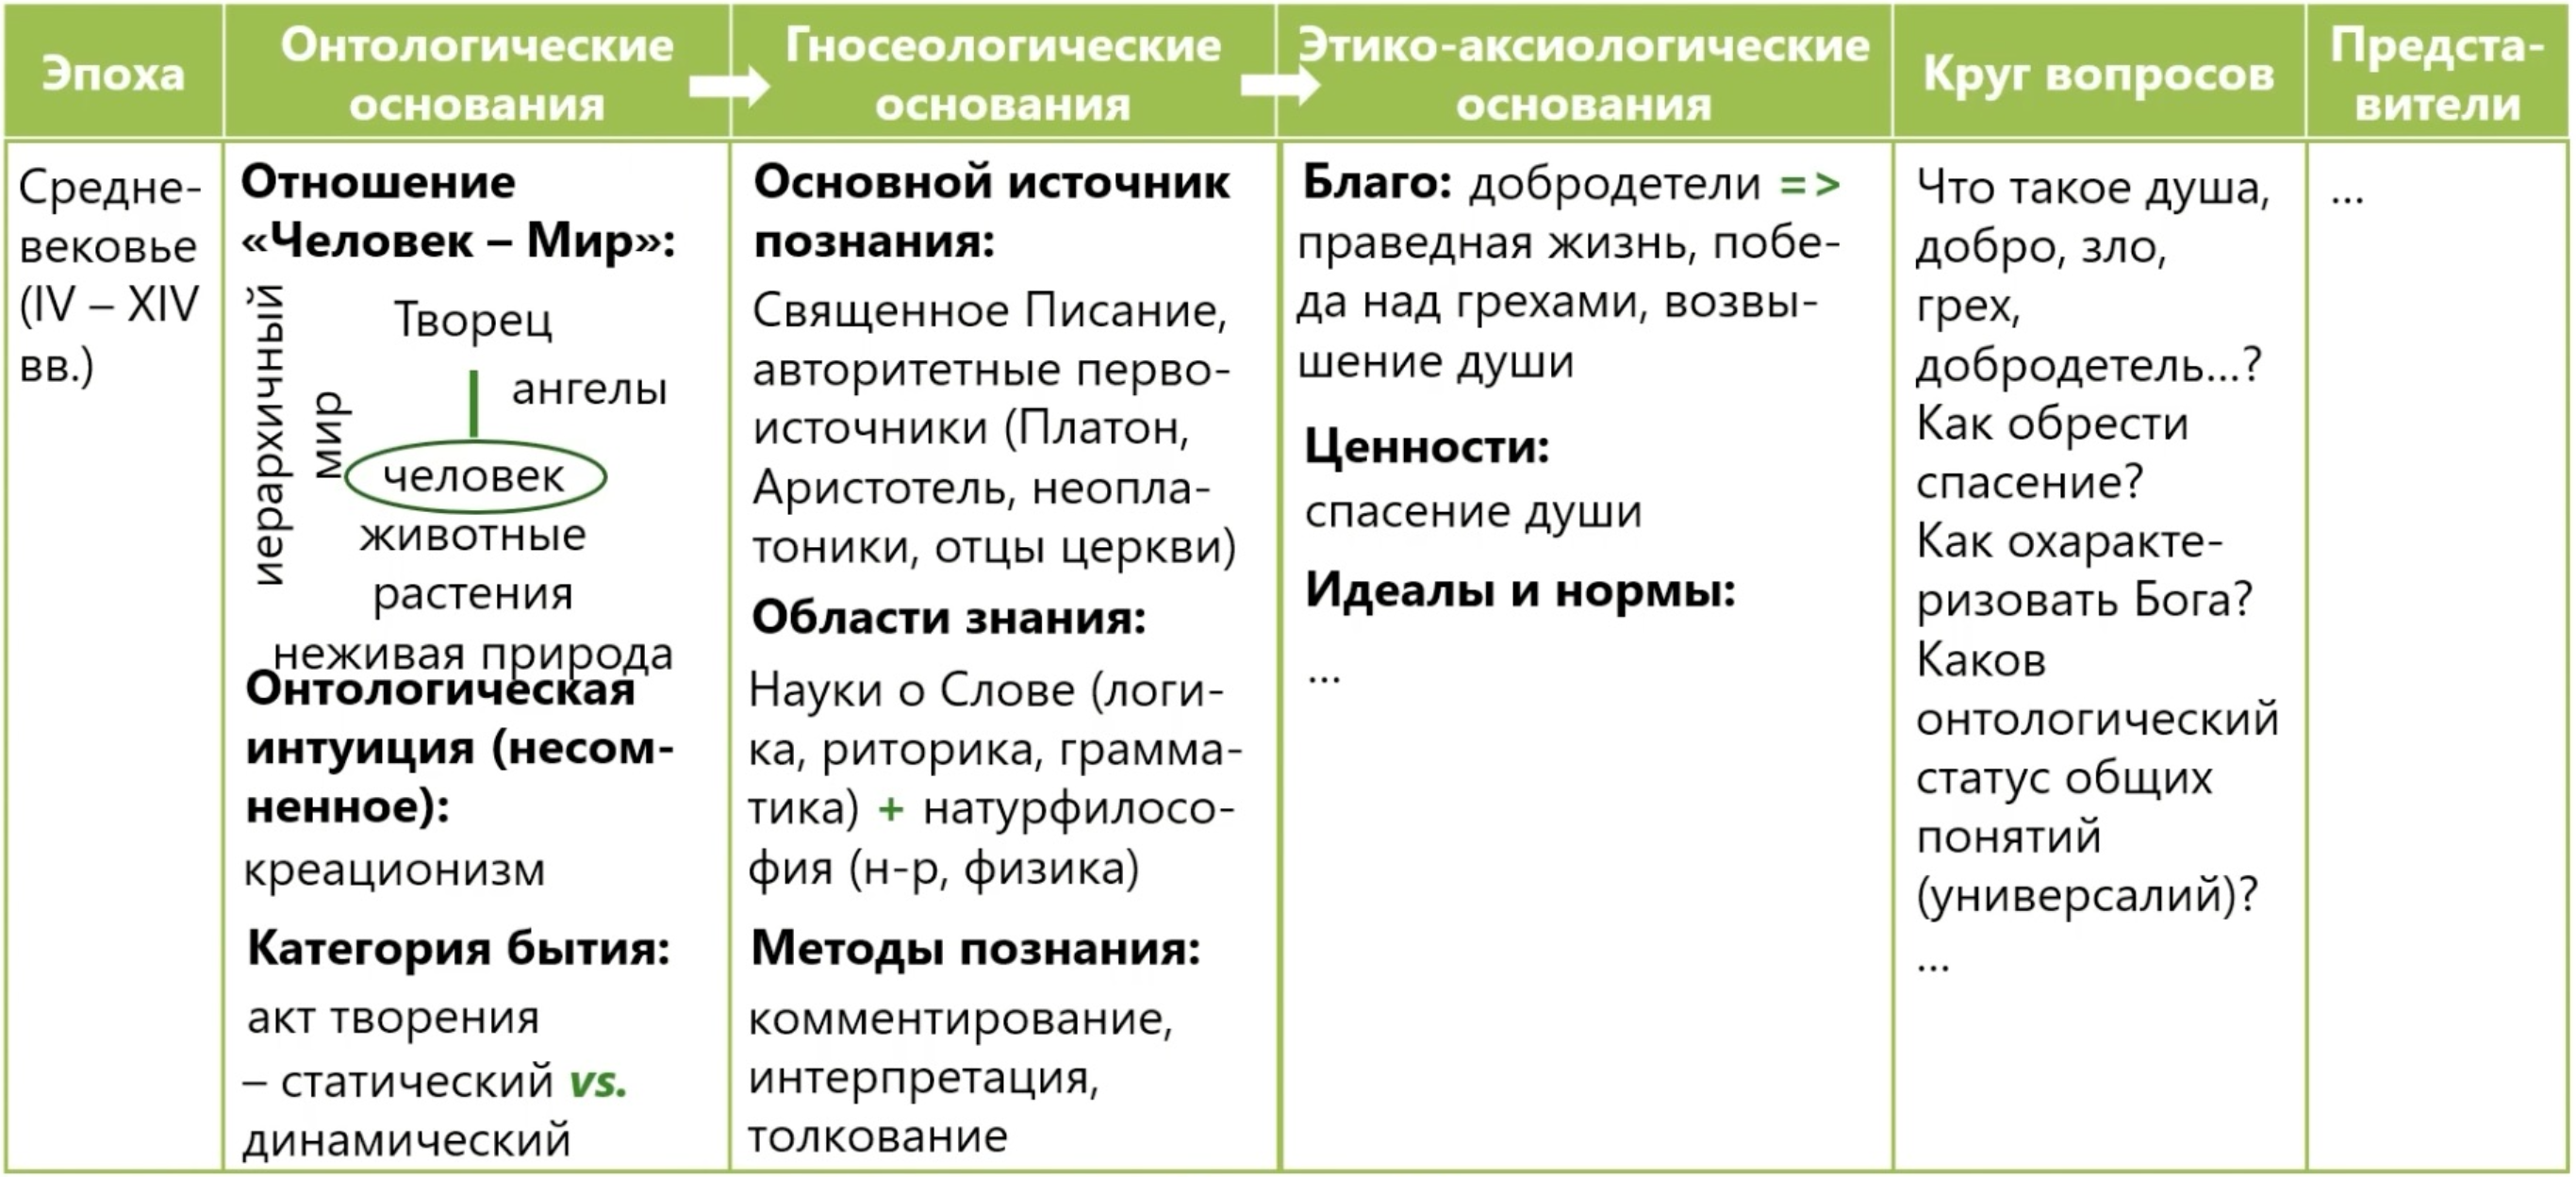
\includegraphics[width=0.8\linewidth]{pictures/med.png}
    \label{medieval}
\end{figure}

Гносеология изучает, как мы познаем. Познанию подлежит всё: от материалов до понятий вроде добра, от природы до Бога. Варианты познания различны, но это всё равно познание.

Эстетика интересуется прекрасным, которое можно увидеть, услышать, ощутить и выразить в разных формах.

Фундаментальные вопросы онтологии: как понимается отношение человек-мир, онтологическая интуиция, что такое бытие (В Средневековье: чистое бытие открывается в акте творения Богом, который создаёт каждую вещь; Бог — само бытие, сущность и существование тождественны; сотворённость мира Богом — очевидная истина.)

Мир Средневековья иерархичен: от неодушевленных камней до ангелов. Человек ниже ангелов, но обладает творческими способностями, будучи созданным по образу и подобию Бога. Мир эстетичен и статичен, но в нём есть динамика изменений.

Главная ценность Средневековья — Бог, а чистейшая часть человека — душа. Цель — спасение души, праведная жизнь. Основное обучение связано с интерпретацией Священного Писания и наставлением к праведной жизни. Познание природы второстепенно; преобладают методы комментирования текстов, авторитетными источниками служат труды Платона, Аристотеля, отцов церкви.

В Срнедневековье развиваются гуманитарные науки: грамматика, логика, риторика, герменевтика, экзегеза. Наука сосредоточена на слове; цитирование и аргументация становятся важными методами.

В античности мир воспринимался как единое целое, часть отражала целое. Например, кусок камня содержит свойства всего камня. В Новое время: целое состоит из частей, и части меньше целого. Декарт: понимание целого через анализ частей.

Каждая эпоха определяет культуру через философские основания. Отношение человека к миру влияет на жизненный уклад и способ познания. Эпохи трансформируются медленно, через накопление критической массы людей с новыми основаниями.

Наука развивается через смену концепций, но истина остаётся неизменной. Видение истины зависит от типа культуры (например, закон всемирного тяготения Ньютона --- истина существовала всегда, но была осознана лишь в XVII веке).

Понимание культуры невозможно без философских оснований. Исторические эпохи характеризуются различными способами познания, что связано с основными мировоззренческими принципами.

\subsection{Историческая проблема «начала» науки и деление на эпохи}

Задаваясь историческим вопросом <<в какой момент возникла наука?>>, прежде
необходимо определить, что понимается под наукой.

% с тем, на возникновение чего мы собираемся искать.
% Интересно, что философия науки, призванная заниматься осмыслением феномена науки
% в его бытийной и познавательной укорененности относительно молодая область
% исследований, начала выделяться в самостоятельную дисциплину, она лишь во второй
% половине XIX века с остановлением позитивизма, а прочное место в ряду
% университетских курсов заняла девушка к середине XX столетия. Такое позднее
% формирование отдельной философской области, посвященное специальному
% исследованию науки, наводит на мысль о недавнем по сравнению с искусством,
% религией, философией возникновении самой науки как специфического феномена,
% привлекающего к себе внимание лишь с недавних пор. 

% Задаваясь вопросом о том,
% когда наука стала такой, какой мы ее сегодня видим, с ее математизацией,
% экспериментальностью, небывалым размахом в плане масштабов внедрения во все
% сферы жизни и деятельности человека, 

Понимая науку как экспериментально-математический способ рационального познания мира, 
мы неизбежно упираемся в основание новоевропейской науки (рубеж XVI-XVII веков). 

% И достаточно распространена в современных исследованиях
% позиция, согласно которой науку считают самостоятельным видом деятельности,
% начиная с рубежа , в силу установления математики в качестве
% фундаментального языка описания природы и эксперимента в качестве ведущего
% метода познания. 
% В результате, отталкиваясь от данных, основополагающих
% концепции, большинство философов науки XX-го столетия обосновывает ,
% то есть науки в новоевропейском смысле. Этот смысл имеет и английская science.
% Как указывают исследователи, с одной стороны, до Галилея и Бекона не
% существовало экспериментов в собственном смысле слова, а с другой, наука,
% предполагающая царство рациональности, становится методологически строгой и
% математически точной, начиная с философии Декарта, положившей именно разум и
% рационально-логические законы пользования им в основании отношения человека к
% мир. Однако, понимание науки как феномена берущего начало в Европе в новое время
% и развернувшегося в XIX-XX веках в тот социальный институт, который сегодня
% повсеместно господствует, ставит обоснованный вопрос о европоцентризме или
% западном происхождении науки как таковой. Представители иных культур, в
% частности мусульманской, вполне закономерно возражают, что те неотъемлемые
% элементы, за которыми современная западная культура склонна видеть свое
% первенство, возникли задолго до XVII века в различных культурно-исторических
% локальностях. Так, например, математика с счетом геометрическими формами,
% которые одинаково для любого сознания человек пользовался по всей видимости
% столько, сколько существует человечество. В Древнем Египте и Мисопотами за 6-4
% тысяч лет до нашей эры на высоком уровне Личили, к примеру, было известно
% процедирование зубов. Были развиты математика, астрономия, фармацевтика, химия,
% сельскохозяйственная наука. В Древнем Китае, помимо остальных известных
% достижений, порох был изобретен не без экспериментирования, как минимум за
% тысячелетия до того, как через ближний восточных алхимиков его рецепты попали в
% Европу и начали активно применяться для изготовления оружия. Арабскими
% исследователями в области математики, алхимии, медицины, экономики и так далее
% многое было открыто и научно описано в 7-13 веках, то есть надолго до
% становления научной профессиональности в Европе. Существование на американских
% континентах до прихода европейцев, мощнейших империй, майя, ацтеков, инков
% невозможно представить без развития у данных народов всесторонней системы знаний
% от математики и астрономии до градостроения или лингвистики, чего стоит хотя бы
% узелковое письмо кипу и скоростная система передач информации инков, загадку
% которой до сих пор не удается понять современным исследователям. Подобные
% исторические факты о научных знаниях и технических достижениях различных

В попытке избежать европоцентризм, многие современные исследователи, задались
вопросом о науке как о феномене человеческой культуры вообще. Наука понимается как вид человеческой деятельности, которая состоит в построении системы знаний о мире. Тогда наука возникла с \textit{появлением человека}, который задолго до изобретения письменности уже
формировал картину мира, познавал и плоды своего познания применял в практических целях.

% И в разных культурно-исторических
% локальностях эти знания могут переплетаться с мистикой, магией, мифологическими
% объяснениями, философскими учениями, религиозными, догнами и так далее. Если мы
% таким широким образом понимаем науку как систему знаний и познания вообще, тогда
% ответ на вопрос о том, когда возникла наука, совпадает с ответом на вопрос о
% том, когда появился человек, который задолго до изобретения письменности уже
% формировал картину мира, познавал и плоды своего познания применял в
% практических целях. Однако, несмотря на свой методологический потенциал и
% предоставляемую возможность рассматривать науку как феномен культуры,
% обозначенная трактовка проигрывает рационалистическому пониманию в плане
% единства и четкости. 

% Невозможно, например, в рамках данного подхода решить
% проблему демаркации научного и ненаучного. Поскольку каждая культура
% вырабатывает свои нормы определения истинности знания, формирует свои методы
% соответствующие формы познания, институционализирует познавательную активность
% свойственные структуры и так далее, знания и познания любой культуры, даже
% далекие от традиционного понимания научности, тогда следует считать наравне с
% иными либо равноправными научными, либо равноправными ненаучными. Наконец, есть
% средний вариант трактовки науки и отчета ее начала, который мы будем далее
% использовать в нашем курсе. Если не любое знание можно охарактеризовать как
% научное, следовательно, не любое познавание окажется наукой. При этом, с другой
% стороны, под вопрос попадает обязательность экспериментирования, математизации,
% объективизации, как неотъемлемых свойств науки. Например, филологии,
% культурологии, истории и другим социумгументарным наукам представляется
% неправомерным отказывать в научности на основании отсутствия математического
% аппарата, экспериментальности и объективности, без чего же наука невозможна.
% Отвечая на этот вопрос, всматриваясь в самое существо науки в своем тексте под
% названием «Нука и осмысление», 

Мартин Хайдеггер определяет науку как теорию действительного. То
есть создание уме, представление, картины реальности, действительного, которое
выражается в научном знании.  Научное знание и методы его добычи впервые четко отделились от ненаучного
мнения как общепринятого суждения в Древней Греции (VII-VI вв. до н.э.)

% Такое определение науки коренится в слове
% древнегреческого происхождения, феория, открывая античный смысл, который можно
% подобраться в нашем языке к отражающему суть синамичному выражению, мысленное
% созерцание. То есть обязательное представление в голове обобщенных
% закономерностей и понимание их причин, а не просто совокупность разрозненных
% знаний или необязательно с математизацией и экспериментированием. Если теория
% отсутствует в основании науки, то математические выкладки останутся пустой
% абстракцией. Эксперимент будет безосновательным, новым совершаемым, поэтому уже,
% срок говоря, экспериментов не будет. Объективные закономерности рассыплются на
% нестыкуемые друг с другом осколки частных представлений. Понимание науки как
% теории действительного, как особого вида познания, которое невозможно без
% специального обращения к теоретическому уровню, позволяет также очертить границы
% науки как специфического вида человеческой деятельности, отделив его от иных
% родов человеческой практики. Древнегреческая философия в ее связи с наукой
% формируется в античности, отделяясь от мифологических объяснений, когда в русле
% менталитета и бытийных интуиций эллинов сложилось понимание необходимости и
% полезности специального практикования усилия мысленного созерцания. 

% Тогда же
% научное знание и методы его добычи впервые четко отделились от ненаучного
% мнения, как общепринятого суждения, которое в греческом называется докса, и от
% чисто практической деятельности, не подкрепленной теоретическим знанием причин.
% Поэтому, безусловно, на таком основании наряду с новым и новейшим временем
% нельзя отказать ни античности, ни средневековью, ни возрождению, как западным
% культурно-эстетическим эпохам в обладании в каждом конкретном случае особым
% собственным типом науки. Но, с другой стороны, развитие теоретической
% составляющей и выделение на данном основании научного познания в рамки
% социальных институтов, научных школ, сообществ, духовных практиков, отделов,
% перформных исследователей, жильцов и так далее дает надежные критерии для
% признания существования науки за пределами западной культурной локальности. Но,
% поскольку в нашем курсе мы именно ею вынуждены пока ограничиться, здесь и далее
% о науке будем говорить как о теории действительного, выделившейся в
% специфическую область деятельности в Древней Греции в 7-6 веках до нашей эры.

\subsubsection{Разделение культурно-исторических эпох в отечественной традиции}

Историю науки делят на два кардинально различающихся крупных периода: \textbf{натурфилософский этап} развития науки (эпоха Античности, Средневековье и эпоха Возрождения) и этап \textbf{научной рациональности}(XVI-XVII вв.: Классическая, Неклассическая и Постклассическая рациональности).


\subsubsection{Разделение культурно-исторических эпох в западной традиции}

Выделяется период Модерна (рубеж XIX-XX вв.) --- отказ от абсолюта, от
Бога, от принятых устоев, традиций, ценностей, от необходимости единого,
устойчивого в культуре в целом и в науке в
частности.

Домодерновый и Постмодерновый периоды выделяются естественным образом.

\chapter{Натурфилософские программы античности I}
 лекции по истории и философии науки. Сегодня мы переходим к самому объемному
разделу нашей дисциплины, который называется «История науки в ее связи с
философией». И здесь, прежде чем начать пятую тему, нам надо затронуть один
важный для понимания целей нашего курса вопрос. Зачем мы занимаемся историей
науки? Почему нам недостаточно познакомиться лишь с современными представлениями
о методологии исследовательской деятельности и ее социальной организации? Это
нужно, чтобы понимать, чем мы занимаемся, когда занимаемся наукой. Сможем ли мы
по-настоящему заниматься наукой, если для нас она будет чем-то не вполне
знакомым? Как можно спросить, сможем ли мы по-настоящему понимать человека, если
толком не знакомы с ним? Мы вроде работаем бок о бок каждый день, знаем его имя,
как он выглядит и так далее, но совершенно не представляем, как с ним быть, чего
от него ожидать, как выстраивать коммуникацию. Точно так же, как про интересного
нам человека, мы хотим знать что-то о его прошлом, причем не просто факты, там-
то тогда-то родился, он столько-то пошел в школу, ходил в какую-то секцию, то мы
хотим узнать о его переживаниях, о его детских воспоминаниях, о его друзьях, его
страхах, кризисах, их преодолении, словом о том, как он формировался, на
основании чего принимал судьбоносные решения и каким образом поступал в сложных
ситуациях. Тогда и информация о датах, цифрах, именах не так важна для понимания
человека. А, собственно, что важно? Важны условия, в которых он рос и
воспитывался, и важны его собственные основания, ориентиры, которыми он
руководствовался в прошлом и руководствуется сейчас. Тогда только мы можем
действительно понять человека и сказать, что это близкий человек, с которым нам
интересно и которому мы готовы уделять много времени, когда мы понимаем
основания его суждений, поступков, выводов. Примерно то же самое имеет место в
случае, когда мы хотим близкого знакомства с делом нашей жизни, буквально с тем,
чему мы посвящаем огромную часть своего времени. Наука не всегда была такой,
какая она предстает сегодня перед нами. Более того, она и сейчас
трансформируется, изобретает новые методы, совершает революционные открытия и
сталкивается с новыми проблемами. Она живет. А понять живое существо в том числе
значит узнать о том, как оно развивалось, на каких основаниях действовало
раньше, на каких и почему действует сейчас. История, лишь по видимости
дисциплина о прошлом, это исследование настоящего в его временной глубине. То,
что здесь и сейчас, не было бы таковым без своей истории, если не только что
возникло. Мы поэтому должны смотреть глубже и организовать наши исследования,
иначе, чем историографическая маркировка тех или иных вех на пути трансформации
научного знания, научной методологии. Сами по себе даты, названия, имена, лишь
точки или пунктирные линии, которыми мы размечаем пространство истории науки. Но
само это пространство не только из них состоит. Оно соткано смыслами. Чтобы
раскрыть для себя эти смыслы, мы должны смотреть глубже и стараться понять
основания того или иного исторического этапа, той или иной культуры, эпохи. Мы
должны научиться у истории науки ставить вопросы и изобретать способы их
решения, вдохновляясь теми проблемами, традицией их обсуждения и ходами мысли,
которые уже до нас и для нас разрабатывали предшественники. Таким образом,
научаясь о истории, мы, самое главное, сможем уверенно выйти к своим основаниям,
которые представляют собой единственный надежный фундамент для наших собственных
суждений, теории и способов поступать. Когда ставится вопрос об основаниях
представлений той или иной эпохи или типа науки, это вопрос о способе
миропонимания, о философских основаниях соответствующего типа культуры. И дело
не только в том, что философия формирует понимание отношений человека к миру,
отталкиваясь от которого каждая отдельная наука углубляется в исследование своей
области реальности. Когда-то между философией и наукой вообще невозможно было
провести границу, они были единым целым. Геометрическими формами обозначались
первоосновы всего сущего, а исследование природы было предметом глубочайших
философских изысканий. Медицинские практики ориентировались на движение небесных
сфер, а бытие описывалось в математических понятиях. Имя этому этапу жизни науки
в её связи с философией — античность. С данной культурно-исторической эпохи мы
начинаем отчёт науки и философии в их совместном становлении в европейской
традиции. Пятая тема курса носит название философской школы «Натурфилософские
программы античности». В рамках данной темы нам предстоит, внимание, две недели
занятий. Античность у нас единственная, занимает на лекциях четыре пары, все
остальные эпохи будут по две. Мы так сделали в нашем курсе, чтобы достаточно
времени уделить самой базовой эпохе, от которой отталкивается вся последующая
европейская философия и наука. Так что разберём четыре экзаменационных вопроса,
к первому из которых мы сейчас перейдём. Второй рассмотрим на второй паре
сегодня, а третий и четвёртый пойдут у нас через неделю на следующем занятии.
Итак, первый вопрос в пятой теме звучит следующим образом. Социально-культурные
условия формирования античной философии и науки. Почему такая именно у нас
логика будет раскрытие вопроса? Мы будем двигаться по нашей схеме изучения
культурно-исторических эпох, который мы разобрали в третьем вопросе предыдущей
темы, перевёрнутая пирамида. Помните, сначала набираем контекст, пишем
социокультурную ситуацию в Древней Греции, времён выделения науки и философии в
специфические виды деятельности. Из этих исторических моментов затем мы
стараемся вывести базовые принципы всего античного мировоззрения и по такому
пути выйдем к фундаментальным основаниям эпохи, антологическим. Так, поняв эти
основания, мы получим ключ, отпирающий дверь к действительному пониманию
философских идей и научных изысканий данного культурно-исторического периода.
Теперь спросим, зачем. В античной философии свёрнута вся последующая философия,
в античной науке свёрнута вся последующая наука. В этот период каким-то чудом
сформировался наш способ мыслить, и какой бы далёкой ни казалось эта эпоха, на
самом деле она в нас сегодняшних глубочайшим образом укоренена. Следовательно,
открывается поразительная перспектива. Изучая основания античного мышления, мы
параллельно сможем прояснить что-то и в своих собственных основаниях, и в
устройстве своего собственного способа мыслить. Итак, начнём с поверхностных
слоёв культуры. Первонаперво нам нужно воссоздать её контекст. Что мы уже знаем
об античности со школы сроков истории и МХК? Припомните, пожалуйста, какие в
целом у вас формировались ассоциации с словом античность. Давайте
последовательно будем отмечать самое общее. Локализуются истоки античной
культуры в Древней Греции, а затем в Древнем Риме. Чётко выделить временные
рамки этой эпохи тяжело. Существует множество вариантов отсчёта, каждый из
которых имеет веские доводы в свою защиту. С начала античной эпохи мы в нашем
курсе условно обозначим с XI века до н.э. С этого момента берёт начало так
называемый Гомеровский период античной истории. Идёт активное формирование
культурной традиции. В своих постоянных чертах оформляются мифы и легенды о
богах и героях. Появляются литературные произведения, посвящённые в частности
странствиям Одиссея и Триянской войне. Это события примерно XIII-XII веков до
н.э. Также с XI столетия до н.э. происходит формирование древнегреческих
полисов, городов-государств, представлявших собой специфические административные
образования, взаимоотношения внутри которых и между которыми также легли в
основании социокультурных особенностей эпохи. Окончание античности тоже
датировать непросто. Обычно отсчёт следующей эпохи Средневековья начинает с
упадка Римской империи, имевшего место в IV-V веках уже н.э. Хотя, например,
величайший философ раннего Средневековья, один из отцов церкви, святой Августин,
жил и творил свои произведения до окончания распада Римской империи, его годы
жизни 354-430 годы. В общем, будем иметь в виду условность такой датировки. На
сегодняшней лекции в плане развития философии Нуки нас будет больше всего
интересовать Древняя Греция, в которой в VII-VI веках до н.э. эти формы
культурной деятельности человека выделили специальную сферу занятий. Римской
традиции первых веков н.э. мы обязательно коснёмся во второй половине занятия на
следующей неделе. Что касается географии, древнегреческой культуры, племена
единого этнического происхождения населяли достаточно обширные территории
Средиземноморского и Черноморского побережья. Древняя Греция или Эллада в те
времена не представляла собой единого государства в той форме, в какой
национальные государства существуют сейчас. Тогда не существовало привычных
межгосударственных границ, а поскольку каждый крупный населённый пункт, полис от
греческого поли, много, но если множество людей, имел в своей власти систему
управления, то фактически по своему статусу представлял собой город-государство.
Тогда сформировались политические отношения, тоже от слова полис, отношения
людей по поводу их совместного проживания, регулирования дел этого сообщества,
внутренней власти и системы управления. Межгосударственные отношения были
буквально межполитическими, то есть выстраивались между полисами. И нередко за
счёт развития дипломатии организовывались союзы таких городов, как для ведения
междоусобных разборок, так и для противостояния внешним врагам, к примеру,
персам, стычки с которыми насушенные на море не были редкостью. Внимательно
посмотрите на карту колоний Древней Греции. Эллины имели колонии в Малой Азии на
территории современной Турции, проникли на восток вплоть до полуострова Крым в
Чёрном море, оставив там знаменитый Херсонес, колонизировали Черноморское
побережье современного Краснодарского края, а также прибрежные земли на
территории современной Грузии. Западные древнегреческие колонизаторы населяли
Сицирию, некоторые территории современной материковой Италии, побережье Испании
и множество островов, окружающих современную Грецию. В рамках этой темы мы будем
обсуждать философские школы, основанные в таких разнообразных местах, как Милет
в Ионии на территории современной Турции, Картон и Элея в современной Южной
Италии, Афины, современная столица Греции и так далее. Как раз на современной
карте я отметила некоторые полюсы, культурные и экономические центры Древней
Греции, в частности гору Олимп, на которой, согласно мифологии, жили боги. Таким
образом, даже уже бросив взгляд на карту, мы можем сделать вывод о том, что
древние греки были отличными мореплавателями и путешественниками, активно
исследовали новые земли, выстраивая с ними экономические и культурные связи за
счет обмена товарами и взаимного обучения. Развитие мореплавания обусловлено
благодатными географическими и климатическими условиями побережья материковой
Греции, изрезано бухтами и заливами вокруг множества мелких и крупных островов,
отсутствуют неблагоприятные морские течения и экстремальные погодные условия. В
полюсах процветали различные ремесла, торговля, занятия искусствами. На обширных
плодородных почвах Средиземного моря развивался седлое земледелие и
скотоводство. Развитие ремесел, искусств в соединении с активным мореплаванием и
колонизацией позволили мощнейшим образом укрепить экономику Древней Греции. За
счет открытия морских путей сообщений появились как восточные, так и в западные
рынки сбыта производимой сельскохозяйственной и ремесленной продукции, а также
предметов роскоши. Надо сказать, что понятие колонизации в случае с древними
греками необходимо отличать от современных наших представлений об этом феномене.
Поскольку в то время не существовало как таковой границ национальных государств
и не было понятия суверенитета, многие земли оставались просто неосвоенными. И
вот на диких побережьях греки высаживались для более удобного осуществления
торговли с другими народами, основывая колонии. Этимологически это слово одного
происхождения с нашим культ культура и означает обработку, освоение. То есть
древнегреческая колонизация с расселением по таким обширным территориям не была
завоеванием чужих земель, а изначально предполагала постройку новых полисов на
неосвоенных землях для абсолютно мирного взаимодействия с другими народами. А к
другим культурам греки относились с огромным почтением, с удовольствием общаясь
с местными жителями, слушая их жизненные истории, знакомясь с их бытом и
мифологическими представлениями. Также и рабовладельческий строй, характерный
для античной Греции, нельзя, на мой взгляд, рассматривать лишь с отрицательной
стороны. Конечно, всякое бывало, и в реальном человеческом обществе во все
времена, независимо от уклада, к сожалению, жестокость неизбывна. Так что
негативные моменты нельзя привязывать ни к конкретной эпохе, ни к определенному
экономическому строю. Но про рабовладение часто говорят о негуманности,
неправильности принуждения и лишении человеческих прав и свобод. Это все верно с
нашей сегодняшней точки зрения. Но для древних греков оно было естественно
сложившейся и глубоко укорененной в культуре традицией, возникшей первоначально
преимущественно по принципу долгового рабства. Когда один человек не был в
состоянии вернуть другому одолженные средства, он даровал господину свою
свободу, становясь его рабом. На самом деле с рабами в ранней античности все
было не так печально, как нам думается. Они могли выкупить себя из рабства и со
временем получить гражданство, то есть обрести статус свободного члена полиса.
Нередкий случай, когда за определенные заслуги господин сам даровал рабу
свободу. Примечательно, что во многом именно благодаря рабовладению граждане
полиса смогли освободить себе время для обучения, развития наук и искусства,
также совершенствования системы государственного управления. Таким образом,
организовав свой быт путем профессионального разделения обязанностей, эллины
преуспели в различных видах деятельности, опережая многих соседей или достойно
соперничая с ними. Это дало не только, как мы бы сейчас сказали, техническое и
военное превосходство. Народ, настолько интересующийся, изобретающий и
совершенствующий формы культурного самовыражения самой своей деятельностью и
идеалами этой деятельности, завоевывал авторитет и внышал уважение. Что еще мы
знаем о культуре Древней Греции? Чем обусловлено ее единство и влияние на столь
обширных территориях? Во-первых, это, безусловно, язык. На древнегреческом
записывались мифы и легенды, создавались поэтические, эпические, драматические
произведения, далась переписка, описывались исторические события, хронология,
генеалогия знатных родов, математические расчеты и исследовательские наблюдения.
Причем желающие могли ознакомиться с этими записями, специально изучать их,
обучаться по книгам. То есть, в отличие от цивилизации, например, Древнего
Египта и Месопотамии, в культуре Древней Греции доступ к передаче знаний,
историческим документам и литературным произведениям имели не только избранный,
обычно узкий круг жрецов и семья проявителя, но все свободные граждане. Так
каждый, в том числе и свободные женщины, могли обучаться тому мастерству,
которое приходилось по душе, от математики до ораторского искусства, от
врачевания до военного дела. И затем уже в свои философские школы женщин будут
принимать наравне с мужчинами, например, Пифагор и Эпикур. Открытый доступ
общества к произведениям культуры в широком смысле к искусству, мифам, истории,
наукам, возможность путешествовать, обучаясь в разных местах и древнегреческий
язык, интегрирующий все эти формы деятельности, безусловно, обеспечивали бурное
развитие всех сфер культуры Древней Греции. Влияние древнегреческого языка на
другие языки, а следовательно и на другие европейские культуры колоссально. Вы
смотрите, я только что употребила слово колоссально, оно древнегреческого
происхождения означает гигантский по размеру. Наверняка вы слышали о колоссе
Родоско. Так даже в, казалось бы, далеком от Греции, нашем Отечестве, в
повседневном обиходе, используется огромное количество слов, происходящих от
древнегреческих корней. До сих пор в обыденной и художественной речи
используются фразеологические выражения, имеющие древнегреческое происхождение.
Даже само словосочетание «крылатые» выражения восходит к Гомеру. «Почивать на
лаврах», «Сизифов труд», «Яблоко раздора», «Петь дифирамбу», «Рок изобилия»,
«Ахиллесова пята», «Ящик пандоры» и так далее. В основном к нам эти отпечатки
древнегреческой культуры пришли через Византию, восточную часть Римской империи,
югром, которая была уже в более поздний период Греция. Возьмем первые попавшиеся
примеры в научном нашем языке, пожалуй, древнегреческих корней не меньше, чем в
обыденной русской речи. Например, «архе» с корнем «арх», обозначающим «древний»,
«главный», «очень». Отсюда «архаичный», «архитектор», «главный строитель». Еще
говорят, например, «архи сложный», значит «очень сложный». Далее. Наши атомы от
«атомос», что значит «неделимый». Наша теория от «феория» – мысленное созерцание
того же корня теорема. Логика, наука логика, с древнегреческого учения о
правильных суждениях или о правильном мышлении. Аризматике от «аритмос» или
«арифмос» в другой транскрипции. «Число», там же корень «ритм» или «рифм», что
является своеобразным языковым указанием на единство музыки со счетом числом.
Кстати, и «музыка» от «музике», что является однокоренным со словом «муза». Муза
– покровительница искусства наук, спутница бога Аполлона. В честь них искусство
в нашем современном смысле называли тогда «мусическими искусствами». А само
слово «искусство» техны понималось более широко, как вообще осмысленная
деятельность человека. Например, искусство землепарца, гончарное искусство,
искусство врачевания и подобное. Искусство как вида человеческой культурной
деятельности, а не в смысле того, что это выражение ощущений и переживаний по
произведению, и как мы сейчас понимаем искусство более узко. Наконец, «психе» –
это душа. Отсюда психология, наука о психике, о душе. Ну, такие примеры можно
приводить еще долго. Это интересное занятие. Вы попробуйте на досуге поискать
другие древнегреческие корни в словах нашего языка, особенно в ваших научных
областях, и почитайте об их происхождении и значении. В таких герменофтических
практиках также должно многое открыться для понимания глубинных истоков
современной науки. Идем дальше. Во-вторых, единство любой культуры
обеспечивается и единством мировоззрения. А что такое мировоззрение? Это то, как
люди видят мир, то есть какие у них представления о возникновении мира, его
структуре и законах, по которым он функционирует. Исторически первой формой
представления о мире является мифологическое объяснение его устройства. Оно
предполагает одушевленный характер всего мира, управления им чьей-то
могущественной волей и сверхчеловеческими способностями. Обычно в мифах также
предполагается хотя бы случавшийся ранее непосредственный контакт божеств или
божественных бессмертных существ с людьми, с миром смертных. Собственно, и мифы
Древней Греции, о которых у каждого из нас есть представления с детства, не
являются в этом плане исключением. Подробнее, мне кажется, о содержании
древнегреческих мифов сейчас нецелесообразно говорить, однако еще несколько
деталей стоит отметить. Самое важное здесь, на мой взгляд, то, что
мифологические представления удовлетворяли человеческую потребность в объяснении
окружающей действительности. Они давали ответы на вопросы о том, как произошел
мир, как он устроен, кем управляется, каким нормам и идеалам необходимо
соответствовать в собственной жизни. И до поры до времени этого мифологического
мировоззрения было достаточно, чтобы существовать и ориентироваться в мире.
Данные особенности мифологического мировосприятия вместе с вниманием древних
греков к языку не могли не отразиться в искусстве Эллады. Для почитания богов
строились величественные храмы из камня в связи с чем развивалась архитектура.
То есть принципы построения зданий используются не только для святилищ, но и для
иных монументальных построек. Снаружи и внутри храмы необходимо было украшать,
поэтому в силу распространения таких наиболее доступных материалов, как камень,
мрамор, глина, металл и сплавы, развитие получали в первую очередь пластические
искусства. Скульптура из камня и бронзы, огончарное мастерство, выкладывание
мозаик, техника росписи фресками и позже камнерезное искусство и,
соответственно, создание барельефа стали основными составляющими
древнегреческого изобразительного искусства. Изображались прежде всего
мифологические персонажи и события с их участием. С другой стороны, устная
передача мифов и легенз способствовала их значительному искажению. Каждый
рассказчик произвольно мог от себя добавлять те или иные детали, допускать
неточности, путать последовательность возникновения богов, в связи с этим со
временем появилась необходимость письменной фиксации взаимосвязи всех
божественных существ древнегреческой мифологии и восстраивания более или менее
единого и непротиворечивого мифологического объяснения мира. Поскольку дела
богов мыслились священными и возвышенными, лежали в основании миропонимания и
несли получающую воспитательную функцию, излагать мифы и легенды надлежала
наиболее высоким стилям в поэтической форме, соблюдении ритма и в сопровождении
музыкальных инструментов. Любовь эллинов к рассказыванию и слушанию историй, к
языку, к речи, ее гармоничному и музыкальному звучанию сыграли ведущую роль в
становлении как словесного творчества, так и музыкальных жанров. Постепенно
совершенствовались музыкальные инструменты и изобретались наиболее подходящие
для того или иного словесного жанра стихотворные ритмы и размеры. Поэты, среди
которых следует обязательно упомянуть Гомера и Лисиона, соревновались между
собой перед публикой выразительности языка, стройности своих сочинений и полноте
передачи в них всех легендарных мифических событий. Собственно, благодаря
сохранившимся фрагментам их произведений мы и имеем современное представление о
древнегреческих мифах и легендах. Распространенными развлечениями с древнейших
времен были также празднества в честь погов с фестивалями и опрядами.
Неотъемлемыми элементами праздников являлись театральные представления,
разыгрывающие поначалу события мифов и сказания о героях Лады, а затем и
драматические произведения с самостоятельным сюжетом, которые постепенно
выделились в отдельный жанр. Спектакли могли быть достаточно длительными, а их
итоги бурно обсуждались зрителями. Самый важный тут момент. Давайте примечанием
отметим, почему так популярны были древнегреческие трагедии, почему собирали
тысячи зрителей в амфитеатрах и на стадионах. Думаю о таких трагедиях, как,
например, Царь Эдип, Антигона, Аристея, все имеют представление. В основе сюжета
лежит социально-этическая опория или парадокс, принципиально неразрешимая
противоречие. Буквально опория означает непроходимость. Слово опора в нашем
языке того же корня, но альфа-приватчевым дает отрицание. То есть опория – это
отсутствие опоры, отсутствие прохода опоры. Так, сталкиваясь с ситуацией, в
которой, в принципе, что бы ты ни выбрал, не получится хорошо для всех, герой
попадает в состояние омехании. Прямой перевод омехании – беспомощность. Такое
состояние ступора, когда мы не можем. Не можем применить никакие механизмы или
техники решения. У нас их много, мы почти все можем, столько всего умеем. Но вот
для этически затруднительных ситуаций, принципиально, нет заранее готовых
решений. И каждый раз нам приходится в конкретике уникальных обстоятельств
сделать выбор на свой страх и риск. Кстати, мы с вами об этом говорили на
третьей теме. Так вот, совместное переживание этого состояния повязанности по
рукам и ногам в таких ситуациях, пронзительное понимание одновременного и
величия человека, и его конечности, смертности, и неумения превозмочь порог
смерти, играло в древнегреческом полисе, городе-государстве роль, простите за
жаргон, таких скреп, на которых держался гражданский дух этого удивительно
мужественного народа. А древние греки и потом римляне, известные своим боевым
духом, побеждали армии других народов численностью до десяти раз превышающей их
войско и лучше вооруженных. Так вот, почему с внешней точки зрения, например,
убийцы своих родителей, Эдип и Арест, все-таки герои? Потому что они мужественно
выдерживают распятие на этой опоре непроходимости, изгоняют в себе пороки, и
благодаря этим чудовищным испытаниям судьбы что-то важное для себя понимают,
оставаясь людьми. Они как бы своей стойкостью, вопреки судьбе и смерти, держат,
выражая словами Мандельштама, место человека во Вселенной. И когда несколько
тысячный коллектив свободных граждан захватывает это переживание, они страдают
вместе со своими героями и понимают, что настоящее человеческое держится только
усилием, стремлением к высшим идеалам и усилием противостояния порокам в себе,
изгнания из собственной души каждым царя Эдипа. Я не случайно здесь произношу
слово «изгнание», оно связано в античном полисе и с такой уникальной практикой,
как острокизм. Голосование, в ходе которого каждый член полиса на общем собрании
писал на черепке или того, кто, по его мнению, наиболее опасен для города, и
того, кто набирал наибольшее количество голосов и сгоняли на 10 лет, как
минимум. Вы понимаете, что этого, естественно, каждый гражданин опасался. Все в
таком небольшом городе друг друга знали и старались для соотечественников
показывать себя с лучшей стороны. Мужчины таким образом буквально соревновались
друг с другом в проявлении добродетелей. Практика острокизма побуждала вести
себя честно, мужественно, справедливо, сдержанно и рассудительно. И древние
греки очень дорожили согласием со своими согражданами в полисе, потому что,
безусловно, изгнание, о котором слухи и сплетни моментально разносятся по
соседним полисам, было страшным позором. А кроме того, потери связей со своими
друзьями и родными, потери своего социального статуса, своего дела и, по сути,
имущества. Очень продуктивная система поддержания порядка, согласитесь. Но
вернемся от нашего углубленного примечания к дальнейшим чертам древнегреческой
культуры, в которых также проявляется соревновательный дух. Богам посвящались,
помимо перов и театральных представлений, многочисленные спортивные состязания
различного уровня и масштаба, известнейшие из которых Олимпийские игры
проводятся в мире по сей день. Спортивные соревнования служили не только в
качестве развлечений и зрелищ, но также позволяли различным полисам
продемонстрировать друг перед другом силу, красоту и способности своих атлетов.
В целом, дух торжества, благородного состязания и возвышенно эстетического
отношения к действительности вдохновлял Эллинов на новые свершения и в силу
такого позитивного соперничества способствовал все большему совершенствованию
различных сфер культурной жизни. Зрелища и праздники, на которые тратились
огромнейшие государственные средства, несоизмеримые по своему объёму даже с
военными расходами, на долгие столетия стали единящим древнегреческое общество
культурным ядром. Как вы понимаете, в любой культурно-исторической локальности
возникает некоторая среда, через которую, как через медиум, каждый отдельный
человек приобщается ко всему своему социуму, чувствует себя его частью и
поддерживает с другими его членами актуальной связи. Таким же медиумом,
например, в средние века выступала церковь. Все члены европейского
средневекового общества в неё ходили, участвовали в обрядах и празднованиях, и
благодаря этому у них поддерживалось такое социокультурное коммуникативное
пространство единых смыслов, в котором рождались и передавались байки и
различные мнения, шутки и серьёзные идеи. Поэтому страшно было отлучение от
церкви. Это означало буквально обрубить для человека возможность общаться, все
его связи с другими людьми. Как если бы нашему современнику, но совсем
заблокировали доступ в интернет и возможность пользоваться мобильной связью, так
что он бы даже электронную почту не мог посмотреть, позвонить родным или
произвести электронную оплату. Вот для нас сегодняшних дома такой средой
являются коммуникативные, цифровые, мобильные системы интернета, особенно
соцсети, мессенджеры и различные платформы, предоставляющие видеоконтент,
возможность трансляции, комментирования, интерпретирования и передачи друг другу
новых актуальных сюжетов. В недавнем прошлом функцию такого медиума выполняли
средства массовой информации, а в нашей стране, в том числе, очень похожем на
древнегреческое общество образом, обязательные коллективные мероприятия вроде
государственных праздников с парадами, субботников и тех же культурных программ,
походов в кино, на концерты, в театр. Так вот, у древних греков подобной средой
тоже были массовые празднества, посещение спортивных и театральных зрелищ, а
также общение на главной площади города, на которой в полисах обычно
располагался рынок. Именно там в основном обсуждались какие-то новости и
политические решения, рождались и передавались мемы, шутки, спледни и так далее.
Кроме того, монархические формы правления архического периода постепенно
сменялись в полисах олигархическими, то есть власть не обязательно передавалась
по наследству. Надо отметить, что древнегреческие правители отнюдь не были
настолько богатыми и богоподобными, как, скажем, персидские или египетские цари,
в полисах власть держалась поэтому в руках сильных духом людей, мужественных,
способных всего себя и всю свою жизнь поставить на карту, рискнуть всем ради
благородного поступка, например, отправиться в совершенно дикие, неизведанные
земли и основать там колонию, организуя при этом своих сподвижников и стараясь
обеспечить для них достойные условия жизни и интересную работу. То есть ценились
прежде всего дела, поступки, а не материальные блага или изнеживающие удобства.
Полисы развивались эффективнее под предводительством Совета, учитывавшего
социально-этические потребности граждан, культурно-экономические и военные
преимущества. Во вновь создаваемых городах на колониальных землях к управлению
гражданскими делами приходили наиболее влиятельные люди, полководцы, стратеги,
знатные и наиболее рассудительные граждане. Они завоевывали у народа авторитет,
покровительство развитию земледелия, ремесел, искусство, торговля и образование,
а также не скупясь на всевозможные развлекательные мероприятия, призванные не
только угодить богам, но и сплотить из сообщества полиса разнообразие в досуг
его членов. Таким образом, к VII веку до н.э. на территориях Древней Греции
складываются уникальные по своей специфике социально-культурные условия,
способствовавшие выделению в отдельной практике особой формы понимания
действительности теоретического мышления. Когда говорят о возникновении
философии и науки в Древней Греции, надо понимать, почему это слово берут в
кавычки. Как мы обсуждали на предыдущих занятиях, вспоминайте, знание как
таковое существовало и передавалось в различные культуры задолго до VII
встаретия до н.э. В Древнем Египте, на Месопотамии и на Востоке, в Древней Индии
и в Древнем Китае известны феномены познания, накопления опыта и передачи
знания. Однако, если можно в этот период говорить о развитии науки, то это была
практическая деятельность, а знание было фактуальным, то есть знанием о фактах,
которые прекращались, прежде всего, в обыденной жизни для тех или иных
практических нужд. И даже, казалось бы, самая теоретическая наука, математика,
использовалась исключительно для применения на практике, для счета измерения
предметов, планирования земельных участков и строительства. Так что мы будем
говорить осторожнее, скорее о том, что феномен теоретического мышления отделился
в эпоху античности от эстетически-мифологического миропонимания. Для понимания
этого ключевого момента давайте, прежде всего, вспомним со второй темы нашего
курса особенности теоретического уровня осмысления. К нему относятся высокая
степень абстракции, необходимая для выделения сущностных повторяющихся черт в
эмпирическом многообразии явлений. Кроме того, если для практической
деятельности характерен непосредственный контакт с объектом, то теоретизирование
происходит именно в уме, не с помощью связи с предметом за счет органов чувств,
но мысленно, независимо от физического ощущения. Так что, когда говорят о
теоретическом мышлении античной культуры, надо понимать, что вовсе не имеют в
виду, что до этого люди не умели обобщать, выделять сущностные причины и явления
или оперировать теми же числами, как предельной абстракцией. Речь идет о том,
что свойственное самой природе человека теоретическое мышление просто не было
систематически развиваемо. Не было до определенного момента самим человеком
замечено как нечто специфическое, как способность, которую развивать необходимо.
Об этом не совсем корректно говорить о том, что наука и философия возникли в
античности и, как в некоторых учебниках пишут, родились из мифов. На самом деле
в Древней Греции к VII веку до н.э. сложился комплекс условий, в которых, во-
первых, мифологические представления не могли дать ответы на интересующие
человека вопросы не о том, как все устроено в мире и каким должен быть человек,
а о том, почему все именно так устроено и зачем человек должен и должен ли быть
таким, как его рисует миф. А во-вторых, культурная и социально-политическая
жизнь побуждала специально развивать и практиковать именно теоретические
способности. Пока вы записываете, я немного прокомментирую, как я вижу эту
ситуацию. На самом деле многие исследователи реконструируют в кавычках
возникновение науки и философии, как именно появление каких-то новых практик в
силу неспособности мифа, как самозамплательную систему отвечать на интересующие
вопросы. Сама формула от мифа к логосу принадлежит советскому антиковеду Тихарио
Харлампевичу Кисиде, греку по национальности, работавшему в институте философии
РАН в Москве. Также подобное понимание характерно для, например, Алексея
Федоровича Лосева, тоже очень известного отечественного мыслителя, исследователя
культуры в ее символическом и эстетическом измерениях. Ну и, например, уже
знакомый нам Мираб Константинович Мамардашвили говорит, что наука не появляется
из простого накопления техник, умений, но обязательно человеку должно стать что-
то непонятно. В мифе все объяснено, и непонятного нет, а проблемность — это уже
черта науки. Но я не совсем с этой трактовкой согласна, поскольку, по-честному,
не знаю, так ли это было, хотя вроде бы логично и обоснованно, что жили себе
столетиями, тысячелетиями люди, пользовались мифологическими представлениями для
ориентирования в мире и не особо задавались вопросами о том, почему все именно
так устроено. А потом такие «стоп, посмотрите, вот непонятно ведь все в мире на
самом деле». С одной стороны, обильная историческая, философская литература
подводит к такому варианту, и нет оснований не доверять нашему гигантам мысли.
Элементарные исторические факты отсчитывают первые, собственно, теоретические,
не художественные, не мифологические произведения с VII-VI веков до н.э. с
Фалесом, Милецкого, Пифагора, Гераклита, Эфесского, Парменида и т.д. Но обратите
внимание, произведения, письменные источники, а как же устная традиция, тем
более в отношении мифа. Поэтому, с другой стороны, мне кажется, не задавались бы
люди вопросами, миф был бы один раз и навсегда. А миф очень текучий, изменчив,
передающийся из уст усталу в слове каждого рассказчика претерпевал изменения,
добавление уточнения, накапливались подробности, развивались все новые витки
сюжетов о богах и героях. Не от того ли, что просто основным, в смысле
привычным, уже сложившимся, средством, инструментом ответа на вопросы был в то
время миф, который можно было трансформировать. Однако, чтобы эту устную
традицию как-то все-таки устаканить, древнегреческие поэты начали в XI-IX веках
до н.э. мифы и легенды записывать. Ведь буква письменного источника тверже
текучести устной речи. Это, по сути, ошибка. Сделать статичным текучее по своей
природе обеспечило настоящий прорыв, который историки и датируют событием в
кавычках возникновения философии. Но на самом деле люди и так уже давно устно
задавались предельными вопросами, пытались для себя что-то понять, удивлялись
чудесно продуманным мироустройству и красоте мира и человека, как и любой
современный человек, но просто не выделяли это занятие в отдельный вид
деятельности и не практиковали специально. В тех же поэмах Гомера уже растворена
вся древнегреческая философия. Большинство философских категорий, встречающихся
в текстах античных мыслителей, слова обыденного языка, которыми и так народ
испокон веков пользовался. Это наводит на мысль о том, что всё-таки, возможно,
философию, науку, теоретические понятия не изобрели и не ввели. Наблюдательные
греки в VII-VI веках до н.э. скорее заметили, обратили внимание на вопрошение и
осмысление как отдельный вид деятельности, наряду с ремеслом, торговлей,
искусством, военным делом и так далее. А в Древней Греции в этот момент
складывалась благоприятная социально-политическая ситуация для осознания
неполноты мифа уже после Гомера Гищода и других поэтов статичного и
зафиксированного явления способности отвечать на предельный вопрос. Давайте
тогда резюмируем всё, что мы тут выше наговорили про начало античной культуры и
уже на более глубоком уровне понимания систематизируем по пунктам эти уникальные
условия того периода в Элладе, которые и побудили греков именно
институционализировать теоретические занятия в качестве самостоятельных видов
культурной деятельности. Развитие искусств, как пластических, так и словесных,
позволило на высоком уровне выражать в письменных и устных формах мифологическое
понимание мира. Во многом этому развитию способствовало поощрение занятий
искусством, а также сложившийся в рамках самого мифотворчества соревновательный
дух. Поэты, скульпторы, атлеты, музыканты, актёры постоянно совершенствовали
свои умения и оттачивали навыки, состязаясь друг с другом. Свобода и
зрелищность, публичность, культура Древней Греции к этому обязывали. В
результате развития словесных речевых жанров активно начали использоваться
художественные приёмы, метафоры и сравнения. К постоянному сопоставлению
обязывала и творческая и соревновательная атмосфера. Как раз сравнение и
сопоставление являются одними из основных теоретических процедур, работающих со
сходствами и различиями. Безусловно, выделение сходств и различий требует
высокого уровня абстрагирования, то есть мысленного одновременного представления
нескольких вещей, событий или феноменов и выделения в них на фоне общего
особенного. Однако к сопоставлению побуждали, как представляются и другие
особенности развития древнегреческой культуры. В силу освоения мореходства и
международной торговли происходило активное знакомство с другими этносами и их
культурами, что побуждало задаваться вопросами о нерушимости устоев собственного
мировоззрения. Другие цивилизации формировались под влиянием других мифов,
соответственно, на иных землях царил свой, отличный от древнегреческого уклад,
формировалось искусство другого типа и распространялись иные представления о
возникновении мира, природе материи и месте человека во Вселенной. Традиции,
обычаи и мифологию других народов греки сравнивали со своими, как мы уже
отметили выше, уважительно относясь к иным культурам и с удовольствием
выслушивая их сказания и предания. Безусловно, тесное взаимодействие действие с
другими народами не пошатнуло мифологические основы древнегреческой культуры,
однако сказалось на широте кругозора эллинов и переосмыслении некоторых моментов
собственного привычного уклада и мировоззрения с учетом опыта других народов.
Полис в качестве специфической формы совместного бытия в древнегреческом
обществе также стимулировал развитие критического и теоретического мышления,
становление олигархических, а затем демократических режимов правления в полисах
постепенно приобщало свободных граждан к вопросам правления, вовлекая в
обсуждение дел полиса. То есть у горожан появилась обязанность помимо
собственных дел заниматься также государственной деятельностью. Общегражданские
собрания проводились на центральной рыночной площади города, которая называлась
Агура. Проводились голосования, направленные на принятие государственных
решений. Каждый при желании мог высказаться в ходе обсуждения вопросов,
касающихся законодательства, полиса, празднеств и других культурных мероприятий,
внутреннего управления, экономических проблем, войны и мира и так далее. Таким
образом, для участия в политической деятельности требовались особые личностные
качества, самостоятельность мышления, критический подход, умение рассуждать,
аргументировать свое мнение, владение ораторским мастерством. В совокупности с
открытым доступом к образованию, что мы тоже уже отмечали, потребность в таком
типе мышления в огромной степени способствовала развитию дисциплин, логики и
риторики, а затем и становлению философского подхода. Все эти условия в целом
дали, как мы бы сейчас сказали, синергетический эффект. То есть совместно
благотворно повлияли на интенсивное развитие рефлексивного и теоретического
мышления, чего в условиях других величайших цивилизаций того же исторического
периода не произошло. Абстрагирование, выделение общего, сравнение,
сопоставление осуществляется умозрительно, то есть не путем практических
манипуляций в мире, но способом воссоздания в своем уме общей формы для
сопоставленных вещей или явлений. Умозрение становится основой, античного
теоретического мышления как метод, с помощью которого можно проникнуть сквозь
видимость к истинной сути вещей. Для чего же был выделен и культивирован этот
специфический способ мыслить? Как мы уже проговорили, мифологическое объяснение
мира, догматическое, по своей сути, не могло объяснить абсолютно все. Человеку
свойственно задаваться вопросами и живая тяга к пониманию никогда не уложится ни
в один статичный конструкт, ни в какие жесткие рамки. Зафиксированная мифология
не давала ответов на многие интересующие человека вопросы. Например, о том, из
чего все состоит, на чем держится единство всего мироздания, что такое добро и
зло, справедливость, мужество, красота, как поступать в противоречивой ситуации,
когда закон велит одно, а сердце подсказывает иное, какова природа человеческой
души и так далее. Ни миф, ни искусство сами по себе ответить на подобные вопросы
были не способны. Однако, несмотря на свою неспособность давать ответы на такие
фундаментальные вопросы, миф и искусство, безусловно, свои собственные функции
выполняли. Поэтому древним грекам вовсе не обязательно было отказываться от
эстетического наслаждения посредством искусства или от мифологического
объяснения вопросов сотворения Вселенной, влияния на человеческие дела. Просто
возникла необходимость осмыслять ряд вопросов другими средствами, чем миф или
искусство. И вот мы с вами сейчас наконец-то подобрались к самым
фундаментальным, глубинным основаниям античной культуры, чтобы ввести
содержатель. Ее онтологические основания мы должны предельно обобщить черты
миропонимания древних греков, о которых сегодня вот уже долго так говорим.
Систематизируем особенности мышления и ценностные ориентиры, которые легли в
основании древнегреческой философии. Итак, фиксируем для себя быстренько. Можно
две колоночки записывать, как представлено на слайде. Любовь к рассказыванию
историй, отразившуюся в мифах, подчеркивала и стремление знать генеалогию, как
происхождение было, так и свою родословную. Отсюда со временем формируется
специальный интерес к поиску причинно-следственных связей и приводит это к тому,
что фундаментальной особенностью древнегреческого типа мышления становится его
рефлексивность, осмысление через последовательную постановку вопросов о
причинах. Древнему греку было интересно все, от новых земель до древних
преданий, от замысловатого движения звезд на небе до отражения окружающих
предметов в мельчайшей капельке воды. Это культура интереса и внимания ко всему,
поэтому в сознании не выстраивалась иерархия окружающих предметов. Не было
различия по степени значимости между всматриванием в ход далеких звезд и
рассматриванием рысинки на траве под ногами, между слушанием дивных сказаний о
богах и интересом к себе смертного человека. Один из лозунгов древнегреческой
мысли, сформулированный первыми философами постулируют все во всем. То есть
отражение одного и того же присутствия, одного и того же события, любого
масштаба, вещи различной величины. Отсюда фундаментальные представления
древнегреческих первых. Мыслили о том, что все, что мы видим, все, что в мире
встречаем, состоит из одного и того же. Следовательно, все во всем может
превращаться. Более того, превращается на наших глазах из куска мрамора в
прекрасную статую, из жидкой массы во вкусный хлеб, из умершего гнющего тела в
плодородный слой, а затем, значит, в нашу пищу, а пища преобразуется в движение
нашего тела и нашего ума и так далее. Все безгранично переходит во все,
поскольку все пронизано чем-то единым. Греки умели восхищаться совершенством и
устройством природы. Стараясь подражать природе в искусстве, они
совершенствовали формы выражения, стремясь к изображению некого законченного
целого. Несмотря на понимание того, что все в мире течет, все изменяется, греки
умели видеть единичность, целостность, воплощенность, полноты в каждой
уникальной вещи. Поэтому целостность и завершенность, ограниченность и
оформленность стали идеалом. Тогда понимание сущего происходило через видение
его границ, его формы, его единичности как завершенности и полноты. В связи с
этим для первых античных исследователей, для всей античной культуры единица не
была числом. В полном смысле слово единица была основой числового ряда, счета,
однако она ценностно превосходила другие числа, составляющиеся путем
суммирования единиц. Важен был предмет в его целостности как своеобразная
единица, которую все и мерили. Также и мир как слаженность целого виделся
упорядоченной самой большой единицей, но тоже единицей. Греки ценили
упорядоченную организацию целого в природе, поэтому в искусстве, а затем в
мышлении в целом. Главнейшими принципами стали гармония и соразмерность.
Ценность имеет целое в единстве своих, пусть и разнородных частей и мерилось все
это философски понятая целостная единица. С ней все соизмерялось точнейшим
образом от пропорции идеальной колонны для храма до разницы в тонах звуков для
благозвучного музыкального произведения. Гармонично упорядоченно двигались
небесные сферы, значит и человек должен стремиться уподобиться этой гармонии
упорядоченной мысли и организуя свою жизнь. Наконец мы готовы ответить на вопрос
об антологических основаниях античной культуры. Напомню, мы их выделяем три. Как
понимается отношение человек-мир, что мыслиться несомненно, и что значит быть в
рамках соответствующего типа мышления. мир представал античному взгляду как
упорядоченная гармонично организованная целая космос. Поскольку же все
отражается во всем, каждая единичность также является полноценным целым. Человек
понимался как микрокосм, то есть как воплощение того же самого порядка, просто
относительно Вселенной более маленького размера. Тогда и во всей человеческой
жизни должно быть стремление к вселенской упорядоченности и соразмерности. Сам
человек должен становиться идеалом совершенства себя как внешне, так и
внутренне. Занятия должны воплощать совершенство, неупорядоченность и
оформленность мышления, а также проговоренность такого мышления, что
обозначается многозначным словом логос, означающим в том числе речь, порядок.
Этическим ориентиром становится добродетель, арите, как неотъемлемое свойство
настоящего правильного разумного человека. Несомненно, для древних греков, не
ставящимся под вопрос, было то, что мы называем вслед за Анатолием Вариановичем
Ахутиным антологической интуицией единого. Для античного человека несомненно,
было то, что все едино. Хотя, обратите внимание, налицо в мире множество
отдельных предметов. здесь демонстрирует свое существо как раз теоретическое
мышление, способное сквозь практическую видимость отдельности и разнородности
умозрительно выявить скрытую от физических глаз связь всего со всем, единства
всего. Раз все едино, для античного мыслителя оказалось очевидным, что все
состоит из чего-то одного. Как бы тогда все могло превращаться во все, например,
как бы мы усваивали пищу, если бы фундаментальным образом не состояли с ней из
одного и того же. Поэтому, задаваясь вопросом о том, из чего все состоит, и
находя разные элогичные ответы первые древнегреческие философы, тем не менее,
были согласны друг с другом в том, что это должно быть что-то единое, одно
начало для всего. Пронизывающий всю Вселенную порядок Логоса не только
обеспечивал своим единством правильную устроенность всего космоса, но и
отражаясь в человеческом уме, как бы настраиваемым на одну волну со Вселенским
порядком, гарантировал человеку способность понимать этот порядок с помощью
разума исследовать законы упорядоченности и соразмерности всего в мире. Так что
этот принцип, замыкающий на себя античное мировосприятие, явился принципом,
легитимирующим саму возможность теоретического познания, что без сомнения важно
для научной мысли любой эпохи. Ведь, чтобы достоверно познавать, нужно
основываться на том, что наше знание не выдуманный плод воображения, но оно
глубинным образом обеспечено благодаря связи наших научных теорий с тем, как мир
устроен на самом деле, наших научных законов с тем, каков настоящий порядок
устройства Вселенной. Конечно, когда мы в следующих наших трех вопросах подробно
познакомимся с идеями античных исследователей, у вас возникнет представление о
плюрализме, то есть множественности направлений. Можно утверждать, что между
мыслителями не было согласия и единства в самых фундаментальных вопросах о
природе материи, первичном, этом же едином, о причинности и так далее.
Действительно, особенно в поздней античности позиции стоиков, пекурейцев и
неоплатоников были непримиримы, они даже демонстративно по-разному стригли
бороды, чтобы подчеркнуть свою принадлежность к тому или иному философскому
направлению. Не искусственно ли мы тогда обобщаем под знаменем единого с большой
буквы всех без разбора представителей античной культуры, тем более столь
длительной и политически неоднородной? Уже у первых атомистов и взявшего их идеи
эпикура в природе базовых начала два атома и пустота их разъединяющая, и у того
же плотина, главного неоплутоника, единая, не только уж единая, распадается на
троицу, проявляясь во Вселенной и также в качестве ума с большой буквы и в
качестве души мира. Вот я сама долгое время пользовалась как штампом этим вроде
бы удачным выражением интуиции единого. Но после тщательного знакомства с
множеством разнообразных первоисточников античных авторов поняла, что правильнее
говорить об интуиции логоса, а не единого. Безусловно, не будет ошибкой
говорить, да если мы сегодня задумаемся над этим, почувствуем очевидность этого,
чем-то единым всё разнородное в нашем мире и правда как-то удерживается вместе.
Душа и тело, например, коллективные, индивидуальные, естественные, искусственные
и так далее. Другое дело, что это непостижимо и почему-то мы упираемся всегда
как минимум вдвоицу, в парадокс, в пары противоположностей. Неприступное это
единое, но всё же даже сам логос логики нас приводит к этому положению. На чём-
то же всё это должно держаться, иначе противоположности схопнулись бы и ничего
бы не было. Так что давайте впредь будем говорить, во-первых, о вкусе античных
мыслителей, к парадоксам, противоположностям, несовместимостям, а во-вторых, о
том, что несомненным для них было именно единство логоса во всём. что можно
своим умом настроиться на понимание фундаментальных законов Вселенной и
человеческого общества, которые, тем не менее, всегда включают в себя
двигательный парадокс, опорю. Наконец, поскольку идеалом был космос, размеренный
и упорядоченный противоположность хаосу, быть в мышлении древнегреческого
человека, по-настоящему быть означало иметь форму, быть целым, завершённым, то
есть имеющим границы, умеренным и при этом соразмерным остальному порядку мира.
Категория меры имеет для понимания античного видения ключевую роль. В
действительности реально быть, быть действовать, значит иметь меру, внутреннюю и
внешнюю соразмерность. Идеал человека быть живой мерой, то есть каждый раз, в
каждой уникальной единичной ситуации как бы примеривать себя к ней, соизмерять
всё и действовать размеренно, умеренно, согласно определённому порядку, а не
имитаться хаотично, беспорядочно действуя и не делать ничего сверх меры. Ничего
сверх меры тоже одна из своеобразных формул древнегреческой культуры. Согласно
такому пониманию, теперь становится ясно, например, почему богатые представители
античного общества, обычно к тому же воскообразованные, одевались скромно, не
пытались чрезмерно украшать свой дом или просто копить свои богатства в виде
золота. Умеренность во всём означало искусство гармонично упорядочивать свою
жизнь, цель которой отнюдь не могла быть мысленна в накопительстве или наоборот
в безмерном расточительстве. Тогда и быть познанным в качестве предмета или
явления мира означало быть включённым в гармоничное целое миро, быть понятым в
качестве оформленного и при этом соразмерного с другими элемента. Всё
беспредельное, а естественно, древним грекам были знакомы математическая
бесконечность и представления о безмерном мыслились существующими лишь
возможности. Их можно было вообразить себе, представить. Однако, поскольку в
мире космосе мы не сталкиваемся с такими вещами, а наоборот наблюдаем
упорядоченность форм и конечность всего внутримирного, то всему беспредельному,
неоформленному, аморфному, безразмерному, неумерному и так далее, античный ум
отказывал в действительном, реальном бытии. То есть, смотрите, при всей
похожести современности на античность, особенно позднюю, что я постараюсь вам
показать на следующей неделе, основополагающим антологическим различием наших
эпох является прежде всего разное отношение к категориям возможного и
действительного. Сегодня нам очевидным и несомненным представляется, что
возможность больше действительности. Ведь мы можем новоображать кучу всего, что
может произойти, чего в реальности непосредственно здесь сейчас нет. И на
основании этого мы поступаем и выстраиваем свою жизнь сплошь и рядом. Например,
живой классик, итальянский современный философ Пауло Лаверно абсолютно верно
подмечает, что, скажем, принимая человека на работу, работодатель смотрит не на
то, что человек реально делает, а доверяет ему, что у того гипотетически есть
способности для выполнения возможных задач. В свою очередь, работодатель обещает
сотруднику тоже возможности карьерного роста и определенных премий или повышения
со временем заработной платы. На деле не факт, что все это оправдается, но мы
полагаемся на такие воображаемые возможности. В Древней Греции надо было на деле
показать свое мастерство, чтобы получить признание, уважение и элементарное
вознаграждение за работу, показать, что ты умеешь, что ты уже реально сделал,
будь то атлетические спортивные трюки или глиняные горшки, песни или лошадиный
упряжь. Мы же на каждом шагу думаем, что у нас много возможностей пойти учиться
туда-то или туда-то, стать тем-то или тем-то, с этим ли человеком сблизиться,
куда поехать отдыхать, какую одежду для кого-то в случае купить. А что на самом
деле, каков настоящий выбор в сфере дел, поступков в мире, а не в голове. И эти
наши воображаемые возможности с удовольствием подпитывают рекламу, пропаганда и
социальные стереотипы. Мы сегодня очень мало смотрим на то, что действительно
здесь, сейчас реально есть. Мало всматриваемся в то, какими мы сами на самом
деле от природы являемся, а не какими нас хотят видеть в этих воображаемых
стереотипах. И, к сожалению, немало людей проживают в жизни, лишь строя планы в
голове и представляя себе, что у них есть возможности. На деле же из-за этого
ничего не успевая по-хорошему воплотить. Так вот, греки видят не так. Они
напоминают нам, что действительно больше возможного. Все наши воображаемые
возможности лишь у нас в голове. Они не имеют воплощения в реальности. А что
реально? Что в мире по-настоящему? Вот это греков интересовало прежде всего.
Конечно, мы отметили, что они первые начали специально практиковать
теоретические занятия, которые как раз именно в нашем воображении целиком
происходят. Но, обратите внимание, для античных исследователей разум
воспринимался как инструмент. Инструмент осмысления действительности, а не в
качестве пространства идолов и мечтаний, которым мы отдаёмся в рабство вместо
жизни в реальности. Безусловно, у человека любой эпохи существует соблазн витать
в облаках и погрязнуть в мечтаниях, не замечая того, что на самом деле
происходит. Однако, сами антологические условия, внимание античности к
настоящему, подлинному, действительному, к природе, как она сама по себе есть и
к человеку, какие поступки он совершает перед лицом сообщества, побуждали, что
называется, заняться делом и воплощать, в том числе, прекрасные произведения
искусства в реальность. Это очень важный момент для понимания всей
древнегреческо-философской научной мысли, поэтому постарайтесь тщательно
запомнить такой ключ к эпохе, антологические основания древнегреческой культуры.
Перейдём теперь в завершение нашего первого вопроса, отталкиваясь от этих самых
фундаментальных оснований эпохи к гносеологическим, этическим и эстетическим.
Интересно здесь прежде всего то, что в античности они были фактически
неразличимы, перетекали друг в друга. Основным источником познания мыслился тот
самый логос, несомненно, антологический принцип, то, что через всё в мире течёт
и всё упорядочивает как в космосе, так и в человеке. Логос — многозначное
понятие. Давайте кратенько здесь раскроем спектр его смыслов и отметим его
логоносеологическое значение для античного способа познания. Во-первых, это
слово или речь. В этом смысле, например, название науки филологии происходит от
греческого «любовь к слову». Во-вторых, не теряя своего значения речи, логос,
как вводилось это понятие первыми древнегреческими философами, мыслился как
некий всеобщий порядок Вселенной, который пронизывает всё своим течением. Логос
и однокоренное с ним лего, как конструктор назван, собираю, означает упорядочно
конструировать. Слушающаяся этого единого порядка природа кампуса образовывает
своё бытие с всё пронизывающим течением космической речи, делающей мир
членораздельным, оформленным. В-третьих, под логосом понимается мысль или
упорядочно оформленное мышление, мышление в понятиях, что на современный манер
можно трактовать как научную теорию. С данным значением как раз коррелирует
название дисциплины логики, которая нацелена на обучение правильности
упорядоченности мыслей и суждения. Сегодня при выяснении темологии название
большинства научных дисциплин, заканчивающихся на логии, типа биология,
психология, геология и подобных, логос в соответствии с данным значением так тут
как учение, что соответствует в частности пифагорейскому оттенку понимания этого
слова. Так, обучение правильному мышлению, настройка своего ума на слышание,
видение, текущего через все единого порядка обеспечивало по мнению
древнегреческих исследователей подключение к логосу как бы программе, которой
запрограммирована вся вселенная. И тогда всматривайся, анализируй, схватывай
порядок и придешь к истинному знанию. Так что истинное знание это логично,
полученное путем умозрительного постижения действительности через рассуждение,
которое обязательно соотносится с тем, как все реально есть, как мир нам
является. Поэтому не удивляйтесь, когда мы начнем рассматривать воззрение разных
античных мыслителей. Они не согласуются друг с другом содержательно. Каждым
авторам предлагаются разные объяснения причин природных свойств материи. Один
будет утверждать, что первое вещество, из которого в разных модификациях
составляются вещи, имеет свойство жидкости, поскольку все течет, изменяется, да
и без влажной среды нет жизни. Другой будет показывать, что в основе всего
огонь, как энергия, которая все в разной степени наполняет своим действием. И
попробуйте на основании современной физики поспорить, что материя в пределе не
энергия. Третий выскажет предположение о том, что материя в пределе число. И все
вещества формируются как отражение комбинаций этих чисел, а главное
соразмерность, гармоничное отношение. И попробуйте, исходя из современных
квантовых представлений о химической связи, поспорить с тем, что соединение не
обязано своим существованием как раз гармоничной согласованности энергетических
уровней, на которых находятся электроны, и которые никак попало образуют связи,
а в строгой порядоченности по определенным квантовым числам. Ну и так далее. Все
эти объяснения реально логично выводятся из определенных основоположений,
которых в рамках своего учения каждый исследователь придерживался. И более того,
звучат равноубедительно даже для нас сегодняшних, хотя и на непривычном языке
выражено то, что мы в своих научных теориях сегодня знаем. Это происходит,
поскольку каждая такая концепция рационально схватывает в действительности то,
что на самом деле имеет место. Другое дело, что каждый схватывает что-то со
своего уникального угла зрения, как бы какую-то более близкую грань в изучаемом
и не может охватить абсолютно все многообразие, выразив в едином
непротиворечивом принципе. Так что конкуренция познавательных конструктов наших
теорий одного и того же это нормально в любое время и античность, несмотря на
стремление к единству и попыткам его схватить выразить, не исключение, а скорее
первая научная эпоха, которая задает такое правило многогранного рассмотрения. И
тут, ребята, до меня на новом уровне доходят идеи Артегии Гассета. Помните, на
прошлой теме я вам цитировала про неизменность истины и изменчивость нашего
знания на примере формулирования Ньютоном законов всемирного тяготения. У Ганса
Георга Гадемера, выдающегося современного разработчика философской герминевтики,
есть подобная идея об истории как истории переосмысления понятий. Мы тоже это
затрагивали на прошлой неделе по поводу разного смыслового наполнения
философских категорий в разной эпохе. И вот банальные вроде бы идеи, но я читаю
античные первоисточники и проводя параллели с современной наукой прямо
прочувствовала на каком-то качестве на новом уровне для себя. Реально, ребят,
смысл знания, прозрение человека в сущность мира, порядка вещей вообще не
меняется. Но язык устаревает, и каждому новому поколению приходится фактически
изобретать новый язык, более понятный, чем те записи прошлого и трактаты
древних. Переоткрывается постоянно одно и то же, потому что логично же,
фундаментально природа не поменялась. Вселенная та же человек, так же
биологически тысячелетия, десятки тысяч лет назад. Но понятая кем-то и
выраженная языком его культуры истина может быть непонятна другому, даже
соотечественнику, скажем, его внуку. Непонятно в силу как раз фиксированности в
каких-то формулировках, уже не работающих для сознания новых поколений в новых
условиях. Конечно, существует прогресс как знания, так и мысли, но некоторые
фундаментальные законы природы и существования человека остаются теми же. Мы
просто сквозь призму своих социокультурных условий переводим их каждый раз на
язык более понятных нам мировоззренческих оснований. Вот поэтому, ребята, мы
изучаем античных авторов. Они уже максимально разработали то мыслительное
пространство для науки и философии, в котором мы до сих пор движемся, из-за
границы которого вряд ли человек выйдет, по крайней мере, пока он человек. По
поводу преобладающих методов познания можно после этого нашего разговора уже
даже не комментировать. Мы только что проговорили о возможном и действительном
вонтологических основаниях. Вспомните теперь со второй темой, чем отличается
наблюдение от эксперимента и соотносите со следующим соображением. Поскольку для
нас современных важнее и больше кажется возможным, в нашей науке с нового
времени процветает эксперимент. В отличие от наблюдения, которое происходит в
естественных условиях, эксперимент создаётся в искусственных. То есть он нацелен
на раскрытие не того, как природа сама по себе естественного действительности
есть, а того, какой она может быть, как она может действовать. То есть цель
раскрытия потенции, возможностей, а не рассмотрения актуальной действительности,
как в наблюдении. Безусловно, каким бы эмпирическим методом мы не пользовались,
теоретическое осмысление будет лежать в основании и для античных исследователей
важно было рационально осмыслить наблюдаемое, сформулировать на логичных
основаниях красивые, предельно простые обобщённые законы, а не просто
зафиксировать описание происходящего, что и так испокон веков до них все делали.
Но самое главное, чтобы вы понимали, я выражу это фразой Анатолия Варьяновича
Ахутина, грекам показалось бы парадоксальным, если бы кто-нибудь решил изучать
естественное, то есть природу и естество неестественными методами. В общем-то,
тоже абсолютно логично. В природе ведь есть только то, что есть, и возникает то,
что возникает, так наблюдай хорошенько за действительностью и познаешь всё. Ведь
возможностей в реальности нет, могло бы быть иным, но не иное, вот такое, какое
есть. И зачем тогда забывать себе голову фантазиями, если мы вот в этом, именно
в таком действительном мире живём, а не в придуманном. Ну а для современных
людей это логические условия такие, что им легко впадать в проживание
ненастоящей жизни, то есть в ненастоящем воображаемом мире возможностей.
Наконец, в этом свете не менее естественно, что знание развивалось обо всём
подряд. Нет, наверное, такого феномена или такого объекта, которого бы не
коснулось этичное любопытство. Так что в эту эпоху было создано знание по всем
областям действительности, зародились практически все наши современные науки, от
физики до истории, от биологии до психологии. Особенностью же эпохи является то,
что не выстраивалась особая иерархия дисциплин, ни в философии, ни в сфере
научного познания, да и между философией и наукой граница не проводилась. Даже
попытавшийся аранжировать по степени значимости для человека дисциплины
Аристотель сам создал головокружительную по своему охвату систему знаний просто
обо всём и равно был захвачен как подробнейшим наблюдением за животными, так и
мысленным созерцанием первопричин всего сущего, как пониманием причин
метеорологических явлений вроде молнии и радуги, так и разбором устройства души.
То есть, можно, безусловно, говорить особенно про позднюю античность после
Аристотеля, что намечается ценностное превознесение метафизики, первой
философии, которая должна прояснять самые фундаментальные первоосновы всего, но
она важнее, поскольку более фундаментальная. И, как Аристотель говорит, без
понимания первых причин любое наше знание будет шатким и фрагментарным. И,
конечно, чтобы упорядоченно мыслить и не совершать ошибок в познании, неплохо
овладеть инструментарием логики. Однако, это просто вспомогательная, буквально,
инструментальная дисциплина. Остальные сферы исследования уже отталкиваются от
определенным образом выстроенной антологической базы, но на которой равна
строится как этика, так и физика, как медицина, так и политика. Что важнее из
этих наук? Вот для античных мыслителей было очевидно и несомненно, что все эти
области одинаково значимы и все их надо развивать. Это дает нам возможность, в
конце концов, плавно перечечь в этические основания и эстетические идеалы.
Принципы разумности, гармоничной упорядоченности, соразмерности, это
одновременно не только антологические принципы, но и этические и эстетические
идеалы. Страшное слово «калок аготия» обозначает одновременно эстетическую и
этическую добротность. Происходит от древнегреческого выражения «калос каи
аготос», буквально «прекрасный и хороший» или «красивый и добрый». Этот принцип
предполагает совместное обязательное сочетание в человеке физической красоты и
добродетельности натуры. То есть был даже такой стереотип, если человек некрасив
внешне, то, скорее всего, он не особо хорош по характеру. Например, Сократа
завистники порицали за его курносость. Это считалось у греков некрасивым, хотя,
на мой субъективный взгляд, вполне обычный, непротивный мужчина, тем более с
отменным здоровьем. Он специально закалялся и регулярно выполнял физические
упражнения, а в Пелопонесской войне принимал участие в качестве гоплита,
пехотинца с тяжелым вооружением, которое носить на себе и которым владеть было
дело исключительных по силе и выносливости воинов. Но своим обидчикам мыслитель
отвечал, что хотя и не подходит к общепринятым канонам красоты, он изо всех сил
старался воплотить в своей жизни, по крайней мере, идеал справедливости,
рассудительности, мужества, внимательности, добродушия и щедрости. Про
умеренность во всем, как принцип жизни, мы уже проговорили в антологических
словах, это, я думаю, тоже особо можно не комментировать. Имеется в виду, что
идеалом античного гражданина было просто при этом опрятно и гармонично
одеваться, не демонстрировать ни умеренность в расходе средств или питаний, а
также уделять внимание равно своему физическому и духовному развитию, чтобы во
всем была пропорциональность чувства, меры и соразмерности, также и эстетический
идеал, который можно, конечно, выразить как красота в простоте, гармонии и
естественности. Очень напоминает, кстати, японский принцип ваби-саби, который
тоже не только эстетический, но и имеет глубокий антологический смысл. Так что
в, казалось бы, совершенно разных и похожих друг на друга культурах мы находим
сходные фундаментальные общечеловеческие основания. Про этический рационализм мы
подробнее обсудим на следующей неделе, когда будем говорить о Сократе и Плутоне.
Но пускай он тут у вас тоже будет в философских основаниях, означает этот
принцип буквально следующий. Если я разумом, а рацию одно да не разум, понимаю,
что такое благо, добро, справедливость, то я принципиально не могу себе
позволить поступить злым или несправедливым образом. Обратите внимание, знание,
гносиологическая категория, неразрывно связано с поступком, а это уровень этики.
Таким образом, подытожим, для античного мышления не характерны разделения таких
областей, как антология, гносиология, этика и эстетика. Поскольку
фундаментальным образом в своей основе всё едино, то ум, красота и добротность
просто разные грани проявления одного бытия. Оно к нам и в каждом человеке
должно являться полнотой, только если всеми оттенками играет, когда человек и
тело своё совершенствует, упражняет, и душу развивает, и разум занимает важными
задачами, рассуждая логично, и поступает по справедливости, по совести. Всё
красиво и стройно. Но, ребят, напоследок примечанием обращу ваше внимание вот на
что. Чтобы у вас не создавались идеализированные впечатления об античности, мы
тут отметили именно идеалы, то есть то, к чему человек стремился. А как вы
догадываетесь, реальные люди сплошь и рядом далеки от идеала, поэтому, несмотря
на высокие этические и эстетические принципы, некорректно было бы превозносить
античность и думать, вот времена-то были, что, мол, все, как на подбор, умные,
добрые, красивые. Реальные античные люди, многие, естественно, как и наши
современники, поддавались соблазнам далеко, не все были симпатичны и
пропорционального телосложения, не всегда могли умерить свой пыл, гордыню,
злогу, нерезко поступали несправедливо и так далее, как и все обычные люди в
любую эпоху. Однако, безусловно, среди них, опять же, как и все времена, были
самые выдающиеся представители нашего рода, которые реально своей жизнью
пытались воплотить эти идеалы, и мы через перерыв начнем, наконец, знакомиться с
теми из великих эллинов, которые посвятили себя исследованиям. На этом завершим
первый вопрос, пятой темы. Всем спасибо огромнейшее за внимание. Если есть
вопросы, с удовольствием отвечу. А ребята, вы тут. Итак, систематизировав в
первом вопросе антологические основания принципа античного мировоззрения,
перейдем ко второму, который в нашем списке к экзамену носит название «Первые
натурфилософские учения античности». Вопрос этот тоже очень объемный, будет как
первый сегодняшний, хотя пунктов в нем мы больше выделяем, просто потому что
множество натурфилософских школ возникло, и понемногу в каждую надо заглянуть.
Чтобы рассматривать сами учения древнегреческих мыслителей, нам прежде всего
нужно разобраться с понятием натурфилософии, которое, к тому же, пригодится вам
в следующих темах. Затем мы должны будем понять, в чем специфика античных
натурфилософских учений, какой круг вопросов объединяет ранних греческих
мыслителей. Следите за заголовочками, как обычно, все пункты сейчас
последовательно разберем. Для начала разберем, что такое натурфилософия вообще.
Существуют две трактовки данного термина. Чаще всего под натурфилософии
понимается философия природы, буквально с латыни «натура природа», то есть это
целостное осмысление природы как общего понятия, через которое, возможно,
становится объяснение отдельных вещей и познание ее фундаментальных законов.
Данное определение предполагает, в частности, что познание природы и ее частей
происходит умозрительно, теоретически, философски, в том смысле, что знание о
природе начинается не с практического взаимодействия с отдельными ее областями и
явлениями, а с построения обобщенного представления благодаря созерцанию
целостной сущности данного понятия и философской рефлексии. Отдельные явления и
области затем изучаются, в том числе эмпирически, в свете такого представления о
природе в целом. Так, натурфилософия, как осмысление категории природы, может
иметь место в рамках любой культурно-исторической эпохи и находит свои
воплощения, например, в метафизике природы нового времени, в стихийном понимании
природы мыслителями романтизма это XIX век, а также в современных
междисциплинарных парадигмах вроде энергетики. Однако, с точки зрения нашей
дисциплины истории и философии науки, натурфилософия представляет собой период
становления науки, берущий свое начало в древнегреческих учениях о первоосновах
и первопричинах мира и заканчивающийся в натурфилософский период в магически-
пантеистических представлениях о природе в эпоху Возрождения. В этом смысле
натурфилософию именно как период развития науки противопоставляют
экспериментальному математическому естественному знанию оформляющемуся с XVII
столетия и последующему развитию науки отграничивающей свою специфику от
философской методологии. Помните на прошлой теме в конце мы делили в
отечественной трактовке историю науки ее на два крупных периода натурфилософский
и период научной рациональности. Так вот в целях нашего курса продуктивно именно
таким способом понимать натурфилософию, поскольку с помощью данного разделения
удобно обобщить особенности нескольких эпох становления науки. Натурфилософский
этап развития науки таким образом включает в себя специфику научного знания и
научного познания в рамках следующих культурно-исторических эпох антично-
середневековья и возрождения. Объединяющими чертами развития науки в данных
периодах являются такие особенности, как преимущественно теоретический
умозрительный подход к познанию. Несмотря на то, что исследователи всегда
наблюдали и проводили опыты, отталкивались они прежде всего от целостных
фундаментальных представлений. Эмпирические методы были вспомогательными и
использовались для уточнения или подтверждения теории. Философское осмысление
природы как целого без четкого разделения на привычную нам область и реальность,
отражающаяся в современном дисциплинарном делении естественных наук. Это
логично. Зачем иерархизировать различные области, если мы изучаем природу как
нечто единое в своем существе? Переплетаться будут все природы, так сказать,
природа камня, ветра, природа превращения и живая природа, природа души. Во всем
будут просвечивать эти единые основания, о чем также следующий пункт.
изоморфность представлений о природе всех вещей вследствие единого основания
понимания категории природы. Изоморфность это сходство различных сущностей по
форме. В данном случае имеется в виду, что в основе любого естественного объекта
или явления видится нечто единое, связывающее его со всем остальным в мире.
метафизическое ориентированность натурфилософского познания. Это означает
преобладание проблематики поиска первоначал и первопричин всего сущего, чем
занимается такой раздел философии как метафизика. О ней мы подробно будем
говорить на следующей теме, когда будем разбирать труды Аристотеля, это он ввел
само понятие метафизики. Несмотря на отмеченные сходства, в рамках каждого
культурно-исторического типа мышления натурфилософия приобретает и уникальные
черты, характерные только для данной эпохи. В связи с этим здесь нам необходимо
для сегодняшней темы выделить особенности именно античной натурфилософии. Для
этого ответим на три вопроса. Как понимается категория природы? Каков основной
источник познания природы? И в чем специфика античного метода познания природы?
Здесь мы также будем опираться и на только что разобранные гносеологические
основания пройдем параллели. В дальнейшем данной схемой можно будет пользоваться
при выделении специфических черт натурфилософии других культурно-исторических
эпох. Итак, прежде всего само понятие природы для древнегреческого сознания это
фюзис. Что это значит? Природа как фюзис природа в широком смысле слова. И
природа вещей, и природа человека, и природа космоса, и природа души. Это
естество. То есть естественное положение вещей такое, как оно нам
непосредственно представляется без специфического ракурса рассмотрения и каких-
то неестественных стесняющих условий. По Аристотелю фюзис противопоставляется
техне, искусству в широком смысле искусственному специальной деятельности
человека, направленной на создание объектов, которых самих по себе в природе не
могло бы возникнуть естественным путем. Аристотелевский пример. Дерево в форме
дерева растет само, а вот мебель из дерева нуждается в искусстве плотника,
столера. Даже если мы воткнем в землю кровать из невыделанных сырых веток,
кровать не вырастет, по природе разовьется опять только дерево, если палки
прорастут. Русское слово природа в этом смысле показательно. Она при родах в
двух смыслах, при рождении, которое происходит само, и при определенных видах
родах того, что возникает. Тогда античная натурфилософия это фактически физика,
исследование того, что, как и благодаря чему есть само. Аристотель, обобщающий в
своих трудах эти представления называет своих предшественников коллег
натурфилософов физиологами, в смысле изучающими порядок природы фюзис. Так что
задача в том, чтобы изучить что и как рождается, в каких видах существуют,
поэтому осмысление движения и преобразования всего сущего устройства Вселенной и
жизни души вещи одного порядка, подлежащие физическому в античном смысле слова
рассмотрению. Основным источником познания природы в Древней Греции, как мы уже
в предыдущем вопросе отметили, про познание вообще, был логос, тот самый
порядок, пронизывающий Вселенную, согласно которому, как и в макрокосмосе, все
было организовано и двигалось определенным образом, так и в человеческом разуме
могло быть все логично отражено, то есть ни миф уже в полной мере не был
источником формирования знаний о природе, ни какие-то другие виды представлений,
например, авторитетные тексты, основным источником было разумное созерцание и
теоретическое осмысление в его соразмерности самой природе, хотя различные
учения о природе формировались, каждый мыслитель все равно подвергал их
осмыслению и соотнесению собственным видением. Античные физиологи от Фалеса до
Лукреция умели начинать сначала с самой природы в ее непосредственной открытости
логическому осмыслению, однако люди, даже в немля упорядоченной вселенской
текучести речи Логоса могут не понимать ее смысл, по мнению, например,
Гераклида, пока не обучаться ясности ее слышания и соразмерному ей проясняющему
рассуждению, в чем, собственно, виделась обучающая функция философии. Для
античных исследователей поэтому не возникала проблема истины, какой она сейчас
стоит перед нами, ведь Логос течет через все, как через природу, так и через
человека, поэтому все возможности для познания открыты, и затуманить его может
только наше собственное нежелание учиться логичности. Тогда как мы можем
охарактеризовать методологию познания природы в эпоху античности? Этот метод
принято трактовать как теоретический, умозрительный, рациональный, логический, в
том смысле, что знание о природе формировалось на основании логически
построенных рассуждений, в рамках которых мыслитель оперировал категориями,
понятиями, выделяя с их помощью сущностные черты изучаемого. Основной первичной
операцией было абстрагирование, то есть выделение из видимого, наблюдаемого
общих закономерностей свойств форм. Предельные абстракции, число и
геометрическое представление, поэтому с ними неизменно переплетаются
натурфилософские учения античности. Однако цель числового и геометрического
выражения представлений о природе недостижения точности или абсолютности, как мы
сейчас подробно посмотрим, греки принимали фундаментальную парадоксальность и
понимали невозможность абсолютного знания. Главное понять упорядоченное
устройство природы в доступных нашему познанию категориях пропорциональности,
соразмерности и гармоничности. Числами и геометрическими фигурами необходимо
уметь оперировать в своем уме в качестве тренировки теоретического мышления или
как объектами, помогающими отвлечь зрение от обыденного наблюдения вещей к их
умственному созерцанию. Короче говоря, математика это как бы язык логоса, того
порядка, которым весь мир дышит и который следовательно человеческому разуму
тоже доступен, если себя соответствующим образом тренировать. И еще одна важная
мыслительная процедура, практиковавшаяся античными авторами, это аналогия. Тоже
однокоренно с логосом. Сопоставление, уподобление, перенесение характеристик,
скользь одних объектов на другие. Буквально аналогия означает равное отношение
равенства логосов. Итак, первые греческие философы начали активно практиковать
теоретическое видение окружающей действительности, задаваясь вопросами, то есть
рефлексируя. И первое, о чем, естественно, было спрашивать, это откуда взялся
мир или с чего все началось. То есть до того, как мифы рассказывают о первых
богах, до них что-то было? Или мир в том или ином виде существовал вечно? Есть
ли у мира начало? Далее в свете интуиция единого логоса спрашивалась о том, из
чего все состоит. То есть было понятно, что все фундаментальным образом из чего-
то одного состоит, но что собой представляет эта единая основа было неочевидно и
в мифах не было объяснено. Наконец, важнейшим был и вопрос о том, почему в мире
все именно так устроено, как нам является. Допустим, все устроили таким образом
боги, однако почему они выбрали и выбирают именно такой порядок вещей, такую
организацию всего, такие цвета, звуки, материалы, формы и так далее. Чем они
руководствуются, делая мир именно таким, с такими красками, такими стихиями,
небесными светилами, особенностями живых существ? Почему не по-другому? Ведь
можно вообразить, что было иначе? Короче говоря, как метко замечает Жиридалёс,
первый философ, натуралист, он говорит о природе, а не о богах. Данный спектр
вопросов образует собой единое смысловое поле проблематики, которое принято
обозначать, как проблема первоначал и первопричин мира. Однако отметим сразу,
что подобные вопросы о начале мира, первооснове, первопричинах всего — это
вечные философские вопросы. Вечные в том смысле, что ими задаётся любой человек
в любую эпоху. Вспомните себя в детстве в вопросе, начинающиеся со слов
«почему?», «как?», «из чего?», «зачем?» никому из нас не чужды. Тем не менее,
несмотря на одну и ту же форму вопросов, в контексте каждой эпохи в определенных
социокультурных условиях ответы даются различные по своему содержанию. Они
оказываются как бы нагружены культурными символами времени, неся также отпечаток
методологии, посредством которой рождались те или иные идеи отвечания на данные
фундаментальные вопросы. К особенностям первых философских сочинений относятся и
то, что они в значительной степени не сохранились, дойдя до нас преимущественно
в изложении и интерпретации более поздних мыслителей. Связано это с тем, что
книги существовали на материальных носителях в небольшом количестве экземпляров,
труды переписывались от руки и таким образом распространялись. Но во время
каких-то войн, природных бедствий или случайных пожаров библиотеки могли быть
разрушены, сохранялись только наиболее популярные, обсуждаемые и цитируемые
произведения. У авторитетных философов естественным образом появлялись ученики и
последователи, которые передавали учения наиболее выдающихся мыслителей. Так
органичным образом складывались философские школы, то есть не специальные
учреждения образования, но спонтанно возникающее сообщества, мыслителей,
учеников и последователей, которые разделяли определенную концепцию. Как мы уже
проговорили в первом сегодняшнем вопросе, отвечать на вопрос о первопричинах и
первоначалах всего можно по-разному. В отсутствии каких-либо ограничений на
свободу мысли сложилось так, что различные мыслители находили отличающиеся друг
от друга ответы на данный вопрос. Все они были достаточно убедительными,
последовательными, логичными, поэтому даже несовпадающие концепции нельзя
называть ложными или выделить только одну из них в качестве единственной
истинной. Различия данных концепций обусловлены тем, что каждый человек видит
мир буквально со своей определенной точки зрения. Никто не может охватить своим
взглядом и учесть абсолютно все. Для разных людей ближайшим и более понятным
оказываются разные вещи, поэтому мы все склонны даже принадлежа одной эпохе,
одной культуре объяснять какие-то вещи по-разному через различные, при этом все
равно умудряться говорить об одном и понимать друг друга. Каждый может через
свое увидеть истину, просто с каждого уникального угла зрения нам будет видеться
несколько иначе. Собственно, такой прорыв к истине нам и важен в философских и
научных идеях. Они подмечают какой-то ход, который, мы говорим, открывает нам
глаза на что-то. Попробуем таким образом познакомиться с различными
направлениями и концепциями древнегреческой мысли. Хронологически первой
философской школы Древней Греции является Милецкая по названию полиса Милет в
Ионии. И первым античным философом считается Фалес Милецкий. Его имя вам
наверняка знакомо со школьных уроков математики. Все когда-то слышали о теореме
Фалеса, о пропорциональных отрезках и параллельных прямых. Без сомнения, это был
выдающий человек с обширными познаниями в различных сферах, путешественник,
получивший образование в процессе своих странствий и изучения культур других
народов египтян, финикийцев, ледийцев. Также известно, что Фалес занимался
торговлей, приумножив свое состояние за счет сдачи в аренду прессов для
оливкового масла благодаря, как бы мы сейчас сказали, экономическому
прогнозированию рынка в совокупности с влиянием климатических факторов на
урожайность. Примечательно то, что во всех сферах своей жизни Фалес
целенаправленно практиковал теоретическое мышление. Например, в 585 году до н.э.
он с точностью предсказал солнечное затмение. Ранее никто этого с достоверностью
не предсказывал. Или сохранили свидетельства, что в Египте Фалес
продемонстрировал свой метод для вычисления высоты пирамиды, которую никто до
него не мог определить, поскольку египтяне не представляли, как можно померить
иначе, чем линейкой. Фалес воспользовался принципом пропорции, измерил длину
тени от пирамиды, которую та отбрасывает в определенный час на ровную
поверхность земли, сопоставив ее с другим, более маленьким предметом, палкой,
длину которой и длину тени, от которой измерить не составляет труда. Так,
сопоставив соотношение длин, он вычислил недостающие, неизвестные значения
высоты пирамиды. Ряд подобных случаев биографии Фалеса буквально обожествил
исследователя, о нем уже при жизни по всей ладе ходили легенды. На самом деле
мыслитель десятилетиями странствовал, обучался, всматривался в действительность
неукасающим интересам, много наблюдал за ходом небесных светил, за погодой,
развитием растений, ростом живых организмов и так далее. А главное, задавался
вопросами о причинах наблюдаемого и старался найти ответы. Это обеспечило ему на
века звание первого в истории философа и ученого. Имя Фалеса неизменно открывало
список семи мудрецов Древней Греции. Считается, что именно ему принадлежит
известнейшее высказывание Гнозиса Автон «Узнай себя или познай самого себя». К
сожалению, сочинения самого Фалеса, как говорят написанные в стихах Гегзаметром,
до нас не дошли, но его учение сохранилось в уцелевших фрагментах его
непосредственных учеников и трудах более поздних мыслителей, ссылавшихся на
произведения милецов. Как философ, пытающийся глубинным образом постичь природу
окружающей действительности в ее единстве и полноте, Фалеса интересен прежде
всего постановкой вопроса о первоматерии или первовеществе, из которой все
состоит и которая им была названа архе, первая древняя иллюзшая в основании. К
VII веку до н.э. у многих народов уже сложились не только чисто мифологические
представления о мире, но, конечно же, и мнения, выводимые из непосредственно
наблюдаемых феноменов, которые мифологизировались. Так достаточно
распространенным было представление о четырех, иногда пяти стихиях, материя и
движение которых образует все видимое в мире многообразие. Данные стихии огонь,
воздух, вода, земля и эфир, как некая высшая спустанция, обожествлялись, с их
силами связывались природные и климатические явления, им приписывались
сверхъестественные свойства. Но с современной точки зрения это аналоги скорее
агрегатных состояний веществ, чем химических элементов, хотя тоже элементами
назывались. Важны в этих первостихиях свойства. Например, землистыми считались
все твердые тела, с водой отождествляя все жидкости, с воздухом все газообразные
тела и так далее. И вот интересно, что Фалес, изучивший воззрение разных народов
на эти стихи, предпринял как раз в свете интуиции Логоса попытку выделить единое
основание для всего. Не считая, что основанием может быть несколько, Фалес
сопоставил известные ему представления с собственными наблюдениями из обыденной
жизни и со своей позиции. Мыслитель увидел воду в качестве первоначала единая
основа всего. без воды все живое вскоре погибает, вода же имеет животворящую
силу, при поливе растения дают хороший урожай, моря и реки дают рыбу, все живое
сдержит влагу, течение жизни похоже на течение воды, и превращение веществ
представляет свой процесс, за течением которых тоже можно наблюдать.
Естественно, вода представлялась в таком качестве в более широком смысле, чем мы
сегодняшние понимаем под этим словом HDO, скорее как влага, вообще как жидкость,
текучая субстанция, которой все наполняется. Другие стихии по мысли фолеса
получались путем превращения воды, замерзая, вода становится твердой, так
поразовались твердые землистые тела, от испарения воды возник воздух, при
чрезмерном перегревании первое вещество переходит в высокоэнергетическое
состояние, становится стихией огнем. На основании данного философского учения
фолес создает, вернее, уточняет имеющиеся мифологические представления о земле,
на которой мы живем, и о небе, в котором наблюдается периодически размеренный
ход светил. Уверенный в том, что все состоит из одной первоматерии, мыслитель
впервые логически выводит, что небесные тела, солнце, луна, звезды, видимые
планеты не божественные сущности, а состоят из того же самого, но они чрезмерно
разогреты, поэтому мы видим их светящимися, горящими. Это на то время просто
революционные идеи. Безусловно, нам сегодняшнее понимание воды в качестве
первого начала кажется ложным, потому что мы привязываемся к словам. Для нас
вода и элемент означают не то же самое, что для древних. Однако обратите
внимание не на содержание учения, а на метод, на логически выстроенное
рассуждение. Тогда становится понятно, что в свете обозначенного нами духа эпохи
и ее антологических оснований из повседневных наблюдений достаточно естественно
было придать именно чему-то жидкому, зримо присутствующему повсеместно, статус
материального, текучего, изменчивого основания мира, из которого все состоит.
учения Фалеса на фоне славы о величии его деяния и его личности привели к нему
множество учеников, жаждущих также постичь порядок мироздания и прикоснуться к
мудрости. Наиболее известными последователями эмилетской школы философии
основанной Фалесом были его непосредственный ученик Анаксимандр и ученик
Анаксимандр Анаксимен. Анаксимандр, судя по сохранившимся отрывкам из его
произведений и свидетельствам о его жизни, был величайшим философом своего
времени, старавшимся глубоко проникнуть мыслью к первосновам. Он многое сделал
своим творчеством для того, чтобы язык философии отделился от художественного
стиля изложения в стихах, а содержание было достаточно самостоятельным от мифа.
В частности, он писал свои труды в прозе. Вслед за своим учителем он задавался
вопросами о первоначалах и, соответственно, пытался рационально объяснить, как
все в мире устроено. Об идеях Анаксимандра сохранилось следующее. Наблюдая
превращение друг в друга четырех стихий, Анаксимандр не счел возможным взять
одну из них за основание, но принял за него нечто от них отличное, чтобы
источник рождения был изобильным. Это особое единое начало всего лежащего
основания мыслитель назвал Аперон беспредельное. Важнейшей категории в культуре
Древней Греции, как мы сегодня уже отмечали, была категория меры или предела.
Мера мыслилась как нечто упорядочивающее, то, благодаря чему все оформилось
именно в таком виде, как это нам предстает. Однако, посмотрите на потрясающую
логичность рассуждения Анаксимандра. В свете вопроса о первичности мера
оказывается вторичной. Она оформляет, ограничивает, а это необходимо делать с
уже чем-то имеющимся. Значит, если ставится вопрос о начале, лежащем в
основании, то есть о том, из чего все состоит, оно должно иметь свойство
неоформленности, неограниченности, чтобы посредством соединения с мерой дать уже
ощущаемые оформленные ограниченные вещи. Также свою первую материю Анаксимандр
наделяет свойствами неуничтожимости и всеобъемлемости. Это потрясающая по своей
логичности и теоретической абстрактности мысль. Анаксимандр славен и многими
другими открытиями и изобретениями. В частности, он первым последовательно
изслужил идею о движущей силе противоположностей. Возражая своему учителю, он
считал, что вечное движение более древнее начало, чем влага, и что благодаря ему
одно рождается, а другое погибает. Из единого выделяются соединенные в нем
противоположности. Рождение происходит не через изменение стихии, а через
обособление благодаря вечному движению противоположностей. О каких
противоположностях идет речь? В мире мы сталкиваемся с ними повсюду. В ощущениях
теплое и холодное, тяжелое и легкое, влажное и сухое, в ходе наблюдений,
рождение и умирание, мужское и женское, большое и маленькое, наконец, в
абстрагирующем мышлении, добро и зло, четное и нечетное, и самое фундаментальное
для максимандра противоположность беспредельного и предела. Эти
противоположности влияют друг на друга и как бы своим неравенством запускают
движение максимандру принадлежит первая формулировка закона сохранения материи.
Из чего все вещи получают свое рождение, в то все они и возвращаются, следуя
необходимости. Все они в свое время наказывают друг друга за несправедливость.
Интересна идея о наказании вещей. Что за несправедливость? Несправедливость в
том, что одна картина занимает собой все пространство. Однако, поскольку все
движется и изменяется, одни и те же вещи не могут постоянно занимать собой все
место. Они должны уходить со сцены в свое время. Так и люди стареют постепенно и
в силу справедливости на их место со временем приходят более молодые. Кстати, о
происхождении человека. Анаксимандр тоже высказал потрясающие идеи, которые
сегодня разделяются большинством ученых в рамках эволюционной теории. В
последствии я говорил о том, что первый человек произошел от живых существ
другого вида, а жизнь вообще родилась в океане, из которого со временем на сушу
вышли существа, покрытые чешуей. Их чешуя лопнула, и вскоре они изменили свой
образ жизни. Поразительно, до какой степени данный маститель умел всматриваться
в природу и замечать, например, сходные черты живых существ разного вида,
предполагая их последовательное возникновение. Аноксимандр также начертил первую
географическую карту известного на тот момент мира, занимался вычислениями,
касающимися движения небесных тел, предложил впервые так называемый небесный
глобус, изображающий движение небесной сферы в кругу Земли, изобрел гномон для
усовершенствования солнечных часов с целью введения измерений и вычислений
посредством фиксации движений Солнца. Аноксимандр постарался уточнить учение
Аноксимандра о первоматерии в свете распространенных тогда идей о логосе как
порядке, которым как бы дышит космос. В сохранившихся отрывках его произведений,
которые были написаны независимословатым стилем и в свидетельствах более поздних
авторов говорится, что Аноксимандр все причины вещей свел к беспредельному
воздуху. Воздух понимался Аноксименом опять же в более широком смысле, однако
наделялся определенными качествами в отличие от Аперона. Для него видимо было
важно показать каким образом происходят трансформации первого вещества, поэтому
он наделил архе вечное и бесконечное свойствами газообразных тел или стихии
воздуха, который как бы вдыхает жизнь во все. В нашем языке, кстати, тоже не
случайно нышать и душа однокоренные слова, а наш нюх одного происхождения с
греческим нус, что означает ум. Так Аноксимен полагал, что из беспредельного
воздуха при разряжении рождается огонь, а при сгущении ветер, туман, вода,
земля, камень. Данные воззрения позволяли наглядно представить смену агрегатных
состояний и превращение вещей друг в друга, та же следует интуиции единого.
Одной из самых многочисленных и влиятельных школ Древней Греции была школа
величайшего населителя Пифагора, имя которого вам также должно быть знакомо
сроков геометрии. Валенекшая в южно-италийском полисе Кратон, пифагорейская
школа распространилась впоследствии благодаря ее ученикам далеко за пределы
одного города, найдя также отклик в сердцах многих выдающихся мыслителей, не
являвшихся непосредственно пифагорейцами. Пифагор, уроженец острова Самос в
Ионии, обучался в Египте и по свидетельствам биографов перенял некоторые идеи,
характерные для древнеегипетской культуры, например, о переселении души, в том
числе в тела растений и животных. Также историки полагают, что пифагор учился у
известного ассирийского мудреца пророка Зоруастро или Зоруастро в другой
транскрипции. Личность мыслителя окутана множеством легенд, однако с
уверенностью можно сказать, что это был мудрый дальновидный человек,
разбиравшийся в людях, умевший убеждать и принимать грамотные политические
решения. За такие способности италийцы верили пифагору и его ученикам управления
полисом. Интересно и то, что пифагорейское учение не распространялось при жизни
пифагора за пределы сообщества его учеников, дававших обет молчания, опознанных
в стенах школы. Однако выдающиеся политические деяния пифагорейцев
способствовали стремительному распространению славы об их тайной школе по всей
Ладе. Также сообщество их славилось особым укладом, у них были общими деньги и
имущества. Учитель сам принимал учеников после беседы, определяя, достоин ли
человек у него обучаться. В том числе наравне с мужчинами у пифагора обучались и
женщины. Одному картонцу Келону было отказано вступить в ряд пифагорейцев по
причине его тиранического нрава. Тогда тот устроил заговор. Собственники Келона
подожгли здание, в котором заседали пифагорейцы. Выбраться во время пожара
удалось лишь двоим самым молодым и сильным ученикам, которые покинули Италию и
поселились на Пелопонесе, решив передавать новым последователям великое учение
пифагора и опубликовать труды. От самого пифагора не сохранилось сочинений,
которые можно было бы приписать ему с достоверностью. До нас дошли отрывки
произведений его последователей, в которых излагались основные положения учения
мыслителя. Однако глубина его философии поражает. Попробуем воспроизвести ее
логику. Размышляя над распространенным тогда пониманием первоначал, как
соединение предела и беспредельного, пифагор не только был захвачен присутствием
других противоположностей во всем правое и левое, мужское и женское, четное и
нечетное, доброе и зло и так далее, но и уловил присутствие единого в основании
этих пар. Если бы не было одного основания до всех противоположностей, основания
фундаментального порядка, согласно которому в мире уже есть разделение, то есть
мы уже сталкиваемся и имеем дело с теми симметричностями, то противоположности
нивелировали бы друг друга, аннигилировали или смешали бы в неразличимую массу.
То есть если бы противоположности и только они были первичны, то, во-первых, это
противоречило бы интуиции единого логоса текущего через всё, а во-вторых,
неясно, что удерживало бы их от смешения и взаимного уничтожения. Поняв смысл
поразительной и непостижимой для человеческого ума задумки природы или
мироздания или высшего разума или Бога назвать как угодно, Пифагор первым назвал
себя философом, а не мудрецом. Пифагор таким образом имел в виду, что человек,
как конечное существо, не может постичь, что предельное основание, благодаря
которому всё существует, потому что оно до нас, не нами создано и не наравне с
нами существует. Его не найти в мире, не схватить своим умом, поэтому он
говорил, что никто не мудр, кроме Бога. Того же, кто желает возвысить свою душу
и стремиться к предельно ясному осмыслению, подобает называть философом, любящим
мудрость или другом мудрости. Слово философия от греческого филия любовь и софия
мудрость на русский язык переводится как любовь к мудрости, буквально
любомудрия. Это любовь к вселенской мудрости, к софии мира, к тому, благодаря
чему всё именно так устроено. По этому поводу замечательный отечественный
мыслитель Владимир Вениаминович Бибихин пишет, что смысл тифагорейского учения в
указании на непостижимый ум, той основы, на которой возникают пары. Когда мы
приходим в мир, то видим сразу правое, левое и другие пары. Увидеть то единое,
которым они выброшены, мы никогда не успеваем принципиально. Тифагорейские пары
указания на нередуцируемую удовольствие на сначала. Нередуцируемую не потому,
что не к чему больше сводить, а потому, что основа пар не наша София. Мы не
знаем и никогда не будем знать, какой Софии создан и почему именно эти, а не
другие морские звезды, которые можно видеть в зоологическом музее. Пифагор ввел
слово философия потому именно, что говорил о Филии, верности такой Софии,
которая другого приобщения к себе, никакой причастности к себе не допускает.
Недоступна эта София, и можно только догадаться об этом и любить ее. Что же это
принципиально меняет? Казалось бы, какая разница, как называть исследователей
первооснов и первопричин мудрец или любящий Софию мудрость, а разница
колоссальная. Представьте себе мудреца, сегодня ведь тоже некоторые люди не
перестают себя выдавать за мудрецов, такой просвещенный говорит, что познал все
законы Вселенной, что в мире 42 ступени различных сущностей, человек это только
четвертое снизу, и надо совершить семь шагов очищения для разных шести типов
людей, но вы поняли, все расписано и посчитано, и нельзя ставить под вопрос. Вот
меня, как философа, всегда такие мудрецы, имеющие, дескать, высшее просветленное
знание, настораживают. Почему? Потому что по определению смертный не может иметь
абсолютно правильного знания обо всем, да и знание о таких предельных вещах
невозможно, не потому что у нас не хватает ума техник напридумывать, но потому
что все эти схемы закрывают собственно человеческое раз и навсегда что-то
определенное о мире и человеке решить, установить, зафиксировать, а наше дело
другое. Во-первых, мир не обязан подстраиваться под наши воображаемые конструкты
и всегда может произойти что-то, что наша схема не описывает. А во-вторых, мы
сами вопрошающие существа и открытые. На каком основании кто-то решает, что все
именно так, что бытие представляет из себя то-то и то-то, как смертные могут
решать, какими быть миру, человеку, чем-то превосходящему нас, предшествующему
нашему рождению. Наш ум, я уже выше говорила, не случайно с нюхом воздуха
математологически связан, а душа с дыханием. Закрывая всю повнуту и все
спонтанное многообразие реальности своими схемами и техниками, такие вот мудрецы
буквально перекрывают душе воздух, дыхание. И в нагромождении их однозначных
объяснений нам становится скучно. Мы задыхаемся, потому что никогда по-честному
не сможем жить в этих закупоренных домиках. Мы ведь творческие существа, а
значит такие, которым обязательно надо новое. Наконец, честнее оставить
открытыми вопросы о том, например, есть ли Бог, неужели мы ему можем указывать,
быть ему или не быть. Возник ли мир или существует вечно? Ведь мы уже упустили
момент начала, родились уже в мире. Что такое материя? А попробуйте ее
определить, если она обладает свойством беспредельности. Если мы не знаем о
таких вещах, может быть, пока не знаем, но вот здесь и сейчас не можем взять и с
наскоку ответить на подобный вопрос. Так давайте, по крайней мере, достойно
поступим, по-честному, сохраним лицо, как настоящие исследователи и мужественно
продолжим держать эти вопросы открытыми. Не спешить впасть в непродуктивные
схемы, повязывающие по рукам и ногам нашу творческую энергию. Так вот, в каком
состоянии дышится свободно? В каком мы счастливы? Не в таком, когда у нас есть
стройное и подробное знание ведания обо всем. А вот любящий не знает, знать и
ведать не пытается, он видит, принимает и понимает. Свободен и открыт, счастлив
в состоянии любви. Ведь что же такое любовь, если не абсолютно доверие и
принятие? Тогда философия принимает все, как оно есть, доверяет устройству мира
и в своем восхищении продуманностью вселенского порядка смиряется с тем, чтобы
фундаментальным образом не знать, как и почему все на самом деле именно так. Мы
любим, например, конкретного человека не потому, что знаем все о нем. Наоборот,
доскональное знание обо всех подробностях его существования скорее будет мешать
его любить. Незнание здесь также имеется в виду не в негативном смысле
необразованности, но в хорошем смысле необязательности модели, конструкции,
прописанной схемы для любимого, принимаемого, видимого. Ведь любим, принимаем,
видим мы не схемы и конструкты, а что-то принципиально не нами созданное, что-то
настоящее, открытое, живое за ними. Хотя без конструкции мы тоже вряд ли можем
обойтись. Другое дело, надо понимать, для чего они нам служат, и каково должно
быть их место в нашей жизни. Но любовь, возможно, только к целому, которая
выбирает в себя парадоксальным образом противоположности в смеси хорошего,
плохого и нас, и мира. Это, безусловно, не значит, что надо заострять внимание
на плохой стороне. Мужество настоящей любви заключается в свободе. Дать
любимому, как конкретному человеку, так и всему миру, быть себе в своей свободе.
А это означает доверить Софии мира, мудрому устройству, чтобы любимое было само
собой устроено, без нашего вмешательства. Тогда мы любим, например, вот этого
конкретного человека, принимаем его полностью, без желания исправить,
переделать, улучшить, залезть в его устройство и контролировать. Наша свобода в
том, чтобы делать свое, показывать пример, тянуться к хорошей стороне, хотя она
не обеспечена, всегда есть и плохая, причем в каждом из нас и то и другое
вложено, независимо от нашего желания. Это удивительно, замечая это все,
парадоксальности и полноте нам дано к такому двигателю из двух неравных половин
фундаментальной парадоксальности всего попробовать как-то аккуратно для
понимания подключаться. Вот Пифагор, видимо, был первым исследителем, который
это четко прояснил. Но подождите, что же в науке ученые не любят? В том-то и
дело, в этом мы все едины. Настоящий исследователь любит свою научную область,
ее методологию, свой предмет изучения. Иначе бы не разговаривал со своими
образцами и приборами, не чувствовал бы их мельчайшего ненастроенность на основе
цели исследования, не сопереживал бы своим респондентам, читая анкеты, не
удивился бы красоте формул, методов, языка. Ученый любит процесс познания, он
захвачен, ему интересно, иначе исследование не настоящее. И его результат в виде
готового знания. Но обратите внимание, в науке мы как бы пользуемся этим
продуктивным состоянием, этим позитивным настроем, чтобы делать свое
исследование. Само наше состояние при этом мы не делаем предметом, мы в его
свете что-то начинаем видеть, понимать и фиксировать в качестве знания.
Философия же, в отличие от науки, можно сказать, наоборот, делает своим
предметом то, благодаря чему оглядывается на само это состояние нашей
человеческой захваченности. Философия угадывает, что состояние нужно
настраивать. И будучи любовью к порядку Софии, призвана нам о таком состоянии
напоминать. Эпифагор был также ученым, на разумных основаниях он старался
создать знания о том, о чем оно нам доступно по поводу природы. Каким же единым
образом можно понять первоосновы всего в мире? Философия Пифагор видел
двоичность предела и беспредельного и понимал логическую невозможность
отождествить одну из стихий с единой первоосновы. Она единая во всех вещах,
похож всепронизывающий порядок Софии или в форме какого-то основы. Тогда на что?
Доступного языка логость течет через наш ум. Ответ Пифагора гениален. Это число.
Число то, что доступно нашему познанию в единой основе всех вещей. Ну, непонятно
вроде, почему вдруг число. Давайте вдумаемся. Число это предельная абстракция,
на которую способен наш разум. Что общего между тремя яблоками и тремя коровами?
То, что их три. Выделяя в обобщающем мышлении одинаковость формы предметов, мы
становимся способны их считать. Так, в пределе мы в нашем уме можем оперировать
числами уже независимо от вещественных коррелятов, то есть математически,
абсолютно абстрактно. То же самое с геометрическими формами. Когда-то поняв
сущность, например, треугольника, мы представляем его в своем уме независимо от
треугольного предмета, а также от того, на бумаге начерчен треугольник, на доске
или на песке. Мы мыслим и в уме оперируем самой идеей фигуры с тремя углами. В
связи с этой способностью нашего теоретического мышления пифагорейское учение и
постулирует число в качестве фундаментальной основы. И число в нашем уме реально
настолько отдельно от вещей мира, что похоже на отдельность единого логоса от
всего доступного нам в империи на опыте. Чувствуете, как близко друг с другом
идут настоящая философия и наука. Благодаря такой аналогии, такому исходному
пункту пифагорейского учения мы обязаны мыслителям данной философской школы
прежде всего развитие математики, строящейся вокруг философских проблем предела
и беспредельного пропорции и отношения подобия и различия форм. Но, естественно,
в свете сказанного пифагорейское учение о числах и геометрических
преобразованиях нельзя понимать, как отвлеченное построение математического
аппарата. Инструментарий этот изобретался и совершенствовался именно благодаря
своей укорененности в философских вопросах о том, как, согласно с какими
принципами и законами все в мире устроено. То есть, не сама по себе математика
была важна, а ее возможности для понимания вселенского порядка логоса, в
соответствии с которым вспоминаете античные антологические основания устроена
как космическая гармония, так и земная, как большое, так и малое. Математика
помогала понять соотношение всего со всем, становилась как бы посредником,
связующим звеном между всеми структурами мира, то есть, своеобразным языком
вселенского порядка. Поэтому, занимаясь математическими абстракциями и, казалось
бы, чисто теоретическими проблемами бесконечной делимости или несоизмеримости
некоторых чисел, античные мыслители на самом деле с одной стороны настраивали
свой ум на чистое восприятие форм, а с другой были захвачены самыми
фундаментальными вопросами нашего бытия и познания, оперируя ими в
математических терминах. В связи с таким особым статусом математики различные
числа и геометрические формы наделялись специфическими свойствами, которые
кажутся непонятными нашему сегодняшнему их восприятию как ценностно одинаково да
и вообще никак не нагруженных человеческим отношением к ним. Единица не
выслелась как непосредственно число. Она была началом и основанием любого счета,
поскольку для того, чтобы начать считать предметы, необходимо выделить каждый в
качестве отдельной единицы. идеал завершенности, полноты, оформленности как раз
соответствует такому ценностному преобладанию единицы как некой самостоятельной
целостности. Неважно какого размера и космос единица как целая, и каждый
отдельный человек единица как завершенность, и каждая отдельная капелька воды.
как пишет один из наших выдающихся философов и историков науки Анатолий
Вальянович Охотин, единицы таким образом для пифагорейцев разновидны и
разнокачественны. Если в области зримых предметов происходит деление единицы, то
она как тело уменьшается и разделяется на меньшие части, но в числовом отношении
она увеличивается, так как место одной вещи занимает теперь несколько вещей.
Помимо единицы ценностно нагружались пифагорейцами и другие числа, в частности,
они полагали число 10 божественным и совершенным, поскольку его составляла сумма
первых четырех цифр 1 плюс 2 плюс 3 плюс 4, она содержала поровну и четных и
нечетных чисел, в конце концов десятками нам от природы видимо удобно считать,
потому что на руках 10 пальцев отсюда пошла наша наиболее распространенная
десятичная система исчисления, хотя вы, наверное, в курсе, что существуют
современные математики и множество других, к примеру, на двоичной построен
принцип действия современных компьютеров. У пифагорейцев числа также
соотносились с геометрическими формами. Единица точка единая целостная, двойка
линия, тройка треугольник, как первая плоская фигура, символизирующая плоскость
вообще, четверка тетраэдр, как первая объемная фигура, символизирующая,
соответственно, трехмерное пространство. По счету углов и ребер геометрических
фигур выводятся все их арифметические характеристики. Равенство сторон,
пропорциональность и симметричность форм мыслятся принципами наивысшего
совершенства. Чем более правильна и проста фигура, тем она божественнее и
прекраснее. Что же может быть идеальнее окружности и сферы? Риторический вопрос.
Поэтому и космос как наиболее совершенное мыслился сферическим, замкнутым, а
движение небесных тел представлялось круговым. Математические исследования
пифагорейцев не были абсолютно умозрительными, находя применение, например, для
описания космоса и для составления теории музыки. Именно пифагорейцам
принадлежит открытие и математическое описание музыкальной гармонии на основании
идеальных числовых пропорций, соотношений. Кто обучался музыке, поймет. Музыка
во многом математика, поскольку для благозвучности необходим точный расчет
интервалов и соотношений высот одновременно извлекаемых звуков. Пифагорейцы
создали основу всей современной теории музыки, исследуя звуки струн, натянутых с
помощью различных грузов, которые в свою очередь пропорционально относились друг
к другу по массе один к двум, два к трём и так далее. Кому интересно подробнее
узнать об этом, почитайте сами, а мы тут подытожим. Поиск пропорций и подобия во
всём характеризуют методологическую направленность пифагорейской школы, гармония
и соотношение. Были интересны этим исследователям во всём, от звучания
музыкального инструмента до устройства Вселенной. Поэтому в заглавии данного
пункта плана я употребила выражение «музыка небесных сфер» отнюдь не
метафорически. Земная музыка для пифагорейцев была способом воспроизводить идеал
космической гармонии, поскольку в своей совершенной упорядоченности космос
буквально так же звучал, как звучат музыкальные инструменты. В школе пифагора
было воспитано множество выдающихся мыслителей и учёных. Заслуги их всех
перечислять интересно, но долго. Поэтому отметим двоих, на мой взгляд, особых
представителей данной философской школы. Алкмен Каратунский был известным
врачом-пифагорейцем, который развил учения о противоположностях применительно к
человеческому телу. Он считал, что сохраняет здоровье равновесие, ибо господство
одной противоположности действует гибелью. К примеру, как избыток пищи, так и её
недостаток вредны для здоровья. То же самое с теплом, холодом, духовным и
физическим развитием и так далее. Это другой взгляд на медицину. В античности
врач-целитель от слова целое, то есть тот, кто помогает человеку быть целым,
целостным, а это как нельзя лучше достигается путём соблюдения баланса и
разумного самоограничения. И действительно, по природе тело стремится к
здоровью, надо только ему не мешать, в том числе стараться, чтобы связанная с
ним душа не тревожилась чрезмерно и с другой стороны не изнеживалась.
Исследовательский интерес к тому, что у человека внутри и как всё устроено в
нашем организме древнегреческим медикам тоже был не чужд. Алкмен впервые
предпринял иссечение, то есть препарирование человеческого тела и благодаря
этому описал, например, как глаза соединены с мозгом с учёт зрительных нервов,
чем доказал в частности, что ощущения поступают в мозг через органы чувств, да и
то, что первенствующая часть души находится в мозге. Алкмен также формулирует
фундаментальное отличие человека от других живых существ. Только он, человек,
понимает, а другие животные ощущают, но не понимают. Филлай, урождённый в
картоне, известен прежде всего тем, что впервые опубликовал основы
пифагорейского учения, которое до этого фактически было тайным и систематически
не распространялось. Филлай интересен тем, что как раз, что благодаря
сохранившимся его произведениям мы много знаем о пифагорейской философской
системе ведения мира с помощью языка чисел и геометрических представлений, а
также о пифагорейской теории музыки. Согласно учению своей школы Филлай понимает
устройство космоса не геоцентрически и даже не гелиоцентрически, но как
Вселенную в центре, в которой находится очаг, огонь, вокруг которого вращаются и
звёзды, и солнце, и другие планеты, в том числе Земля. Вообще я поражаюсь
глубине античной мысли, когда, например, читаю у Филлай, что космос питается
испарениями вылившихся светил, чем не испаряющиеся чёрные дыры современных
астрономов. Когда смеются над воззрениями древних греков и считают их зачатками
науки, значит, не понимают, насколько наши сегодняшние научные представления
повторяют сказанные античными мыслителями. Вроде бы смешно считать, что всё есть
число или всё состоит из некой единой первоматерии, но давайте присмотримся и
вдумаемся на вопрос, из чего всё состоит. Наши современники отвечают, что из
молекул и атомов, а специалисты уточняют из энергии, потому что современная
физика выяснила, материя на микроуровне энергия. Те самые элементарные частицы,
из которых всё состоит, в пределе представляют собой энергетические уровни или
энергетические состояния. А что такое энергетические уровни? Это числа, решение
уравнения Шрёдингера для волновой функции, значит, материя в пределе число. Но
постойте, об этом с конца VI века до н.э. говорят пифагорейцы и вслед за ними
Плутон. Берём примерно более высоком уровне организации материи, если нас сами
элементарные частицы не удовлетворяют. Образ любого живого существа с
определенными особенностями передаётся от родителей детям, как с помощью
генетического кода. А код это шифр, последовательность, которая тоже число или
числовой ряд. Так что мы с вами как ни крути, тоже в пределе число. Пифагорейцы
оказались правы. Другой пример современной физики. Теория струн очень напоминает
пифагорейские струны с их пропорциями. В общем, советую задуматься над таким
современным стереотипом, что наука ступенчато развивается, и в каждую новую
эпоху знания становятся всё точнее, лучше, правильнее. Мне кажется, реальные
люди в каждую эпоху не садятся с грустью дожидаться, пока же наконец пройдём мы
современные со своими новыми теориями и техниками. Они сами стараются всё
исследовать и понять, сами формируют свою понятную им картину мира. Это нам
сегодняшним могут быть непонятны античные первоисточники, если мы не настроились
увидеть смысл в них вложенный глазами оснований этой эпохи. На деле далеко ли мы
сегодняшние ушли от античных мыслей? В начале предыдущей пары я неслучайно
говорила, что вся наука, в том числе сегодняшнее свернуто в идеях
древнегреческих мыслителей. Может быть действительно историчность языка описания
просто создаёт видимость прогресса? Гераклит из Эфеса. Ребята, один из самых
неординарных мыслителей всех времён вообще. Он взял на себя миссию критиковать
тех, кто мыслит нелогично и в своём полисе одёргивал поддающихся стереотипам и
невежественных. Вёл Гераклит себя достаточно резко и эмоционально. По словам
современников, но был знатного происхождения. В юности путешествовал, сам много
исследовал и его уважали за глубину его философии, которой он не учился у кого-
либо из учителей, но всё постиг самостоятельно. В Эфесе к власти пришёл тиран и
изгнал из города друга Гераклита Гермодора. Маслитель призывался граждан
препятствовать этому, но они не стали сопротивляться. Когда же потом в спорной
ситуации к нему играющему с детьми у храма Артемида прибежала взволнованная
толпа сограждан и попросила дать им новые законы, Гераклит остался играть с
детьми, сославшись на то, что город уже во власти дурного государственного
устройства. Афиняне приглушали мыслителя поселиться у них после того, как эфесцы
разобиделись на своего философа за подобное поведение, но он предпочёл остаться
на родине. Даже персидский царь к нему и его друзьям пожелал приобщиться к
мудрости Гераклита и приглашал его переселиться в Персию под свою опеку.
Гераклит себя и с царём держал на равных, переписывался с ним, сохранились
несколько их писем, сообщал о своих идеях царю, но от приглашения отказался,
слишком был свободолюбив. Гераклит не основал своей школы, от его философии до
нас дошло всего 139 фрагментов, в основном афоризмы, но чуть ли не во всех
последующих учениях можно проследить влияние его мысли. Например, Гегель как-то
сказал «нет положения Гераклита, которое я не принял в свою логику». Гераклит
назвал то самое единое начало Логоса и полагал, что этому первичному похожему на
речь порядку подчиняются и боги. Логос один и тот же во всём и для всего. Не
уступая Пифагору в глубине философской мысли, Гераклит говорил, что мудрость
София, которой всё устроено отдельно от мира и настолько иная, что мы себе не
можем её представить. Видим только уже отражение противоположностей в нашей
Вселенной, их движение, их игру. Другое всему отдельное это та половина
Гераклитовской мысли, о которой Сократ сказал, что он её не понял. Чтобы понять,
нужен, пожалуй, говорит он, дозвский ныряльщик, но что она так же подлинно, как
половина Сократа понята, сомнений у него нет. Не поняв, то вторую половину
Сократ отнёсся к ней тем единственным способом, какой достойный ныряльщикам.
Отдельно таково, что в нём нет ничего отвечающего приёмам человеческого
поздания, как под водой нет воздуха для дыхания и надо быть искусным ныряльщиком
не для того, чтобы найти способ пребывания на глубине. Это невозможно, а только
для того, чтобы не сразу задохнуться там. София другое разума, так же, как и
другое неразумие. Для нас другое жизни, смерть, но для гераклита это единое
основание настолько другое, что оно иное и смерти. Это иное мы не можем понять.
Оно одно отдельно. По гераклиту настолько, что оно другое одновременно и богам,
и людям, которые, казалось бы, противоположны друг другу, как смертные и
бессмертные. Захватывают такие прозрения. Другое таково, что не может быть
истолковано и продемонстрировано, стала быть, наша задача не в понимании или
непонимании, главное, в нашем завязавшемся отношении к другому. Не даром
гераклит не хочет ничего описывать и рассказывать. Он говорил, что Гомера и
Археолога надо бы высечь за то, что их мысль вязнет в мифологии, в рассказывании
историй. Так что, например, фрагмент 90. Огонь обменивается на всё в мире и все
и всё на огонь, как золото на вещи и вещи на золото. Эту потрясающую по красоте
лаконичности метафора Гераклида вовсе не обязательно трактовать только как
первую формулировку закона сохранения энергии, хотя это тоже, естественно, есть.
И о космосе и его фрагмент 30. Космос был всегда, есть и будет огонь вечно
живой, зажигающийся соразмерно и гаснущий соразмерно. Не обязательно речь о
концепции пульсирующей Вселенной, одной из концепций развития Вселенной в нашей
современной космологии. Гераклид прямо говорит в 64 фрагменте «Всем сущим правит
огонь, в смысле энергия, которая у мыслителя молния». И еще одна
головокружительная фраза об этом, 11 фрагмент «Все живое пасется молнией» или в
другом переводе «Все ползущее бичом пасется», точнее было бы сказать «мгновенным
ударом». В оригинале там «плэгэ», резкий удар, который во всей греческой
литературе известен как удар молнии Зевса. Так что же, сам наследитель вязнет в
мифологии и решает, что главная сила, управляющая всем во Вселенной молнии, как
бы не так. Давайте присмотримся. Гераклидовский логос, как сосредоточенный
смысл, помните логос от лего, собирая, правит по способу молнии и сам есть
молния. Как мгновенно может править многим? Возможен ли логос как молниеносное
захватывание всего одним? Логос не имеет отношения к обобщающей, абстрагирующей,
рационализации сущего. Он подобен не описи мирового богатства, а его золотому
эквиваленту. Он поэтому не хуже вещей, подобно тому, как золото не хуже товара.
Так что, продав вещи, получив в обмен не их список, а хорошую цену в твердой
валюте, нет причин грустить о них. Огненный логос то золото, которое заранее
знает цену вещам. Золото логоса не условно и схематично, а по существу выбрало в
себя своей непостижимой внезапности все вещи. Золото стоит вещей для вещей, но
их высшая возможность. Они исполняются, узнавая себя в молнии своей тайной и
истинной сути. Молния исполнения вещей, потому что они хотят вторить ей,
тянуться, слиться с ней. То есть, как понять, эта молния всем правит? Это
вертикаль чистого момента теперь по отношению к горизонтали нашей хронологии.
Это вот здесь и вот сейчас как единственное настоящее. В чём оно? В действии. А
это в деле, в действии перевод греческого слова энергии. Вы знаете, как вдруг по
осени разом птицы сбиваются в стаи и пускаются в тысячекилометровый путь? В
общественную государственную жизнь не правит сходный закон. Например, в нашем
Отечестве сообщение, переданное ранее весной 1917 года из отдалённой столицы по
всей стране действовало не своим содержанием, убеждало не обещанием
переустройства жизни на более разумных началах взамен старым и нерациональным.
Сообщение было принято страной как сигнал. Оно вгоняло человека в другое
электризованное состояние. Современники отмечали, что человеческий тип в России
сменился за несколько недель, если не за несколько дней, часов. Все вдруг
поняли, что пробил час. Но длительное до этого существование восприняло импульс.
И далее проблема передачи власти, любой, не только монархической. Молния не
передаётся никак, ни по наследству, никаким другим способом. Молнией можно
только самому быть. Это тяжело настолько же, насколько уместиться в границе,
которая ничто любому что, в чистом различии, где нет пространства. Помните, мы
на третьей теме говорили о призывании, о совпадении с собой? Не могло оторваться
от Гераклита, но приходится. У него ещё множество бездонных фраз. По ссылкам
внизу обязательно сами прочитайте. Мы тут только одним глазком заглянули, но,
надеюсь, молния хотя бы на миг озарила и позволила увидеть, какой величины это
философ. Под стать ему его не менее выдающийся современник с другого конца
Эллады рубежа VI-V веков до н.э. Парменит из Элеи на юге Италии. Сразу отмечу,
что в оригинале на древнегреческом сохранился лишь небольшой отрывочек его поэмы
о природе, но в этих строках спрессована просто вся последующая философия,
столько смыслов, что ни в один перевод не влазит, и никто не может передать весь
размах парменитовской мысли. О его тексте не утихают споры, появляются новые
интерпретации, комментарии, новые развороты, обсуждаемых парменитовом вопрос. Я,
конечно, за несколько минут не смогу вам развернуть весь этот масштаб, мы лишь
коснемся самых базовых моментов, о которых принято говорить про парменида. снова
отошли у вас читать Владимира Вениаминовича Бибихина, этого уникального,
мощнейшего отечественного философа, который во всех своих работах потрясающе
осмысляет античных авторов, идей парменида, много где касается, но самый
головокружительный, захватывающий разбор в чтении философии. Парменитовский
текст в греческом оригинале составлен из точнейшим образом подобранных слов, о
мистическом опыте, постижении самого главного, того единого, что одновременно
любовь, истина, смысл, чему мы все как бы принадлежим. Ни один его перевод уже
не может передать всей этой точности, всего размаха его мысли, но хотя бы в
переводе, что нам осталось от парменида? Он впервые обратил внимание на то, что
та отдельная от мира единая основа всего не есть нечто. Ответ на вопрос что? но
само это есть или быть бытие, которое присуще всему вообще, что было, есть или
может быть возможности, причем в одинаковой степени. В связи с этим говорят, что
параминит ввел в философский язык понятие бытия, хотя, конечно, мы должны
понимать, что эти слова быть, есть в любом языке с момента его возникновения,
есть. Но параминит обратил внимание на то, что самое главное, самое отдельное от
вещей и непохожее на них бытие. Усердно упражнявшийся в зрительном подходе,
многое читавший, видевший, знавший. Параминит как бы отпускает свою мысль,
жаждущую истину. В начале поэму он образно пишет, что его несут кони в
колеснице, стремительно к свету этой истины. Вопрос об основаниях приводит или
приносит мыслителям, благодаря предельному теоретическому абстрагированию, к
видению того, что небытия нет, то есть всё есть и не быть никак невозможно. Он
открывает, что небытие для нас имеет место лишь по видимости. В мире мы
наблюдаем рождение и смерть. до рождения и после смерти нам кажется, что имеет
место небытие. Но параминит вызывает нас внимательнее присмотреться. Тело,
скажем, человека, ведь не появляется из ничего и не исчезает абсолютно в никуда.
Какие-то процессы приводят к возникновению, затем к гибели. Но это, по сути,
лишь качественные резкие изменения того же самого. То есть у нас создается
впечатление, что бытие сменяется небытием, а на самом деле мы наблюдаем
постоянное превращение бытия, смену способов бытия. Просто для нас жизнь
ценностно нагружена по сравнению со смертью. Однако по природе умершее тело
просто переходит в иное качество, разлагается и становится питательным веществом
в почве, благодаря чему что-то тоже может родиться. Сегодня умершие миллионы лет
назад живые организмы для нас топливо, одежда, пластик, то, во что
перерабатывают нефть и уголь. Так что по параминиту можно сказать, что древние
жители планеты не в небытие канули, а преобразовались и никуда не исчезая
сегодня, служат для нас вполне ощутимыми вещами. Так же и рождение существа
происходит не вдруг задолго до появления на свет и создается зародыш, который
питается и растет. До физического своего появления он пребывает просто в другом
качестве, но это тоже бытие. Головокружительная мысль. Во-первых, все уже есть и
прям совсем исчезнуть не может, а во-вторых, весь мир, природа вся как бы творит
себя, постоянно преобразуя то же самое, но перекомбинируя, попробуя новые формы.
Так все развивается. Параминит говорит о бытии, и неделимо оно, коль всецело
подобно. Тут вот не больше его ничуть, а там вот не меньше. То есть везде, во
всем на самом деле одинаковое бытие и в качественном, и в количественном
отношении. Чтобы мы не ткнули, везде упремся в бытие. Нигде не получится найти
ни бытие или ничто, всегда будет обнаруживаться нечто, хотя бы даже это само
наше ищущее стремление. И тут мыслитель в одной своей формулировке сворачивает
основную идею всей последующей западной философии. То, чего нет, нельзя ни
познать, ни удастся, ни изъяснить, и помыслить тоже, что быть. Напоминает
Декарту формулу, я мыслю, следовательно, я существую, но Декарт, конечно, не
воспроизводит Параминита специально, а заново, с нуля, с чистого листа,
осмысляет то же самое, но в своей уникальной культурно-исторической ситуации,
приходя к той же истине. Параминит говорит, можно ли что говорить и мыслить, что
есть. И если уж нам удалось увидеть истину, тогда то же самое мысль и то, о чем
мысль возникает, ибо без бытия, которым ее изрекают, мысли тебе не найти. То
есть и мыслим мы только осущим, и бытии, пусть и встречаются они нам в разных
модусах. С той колеи, по которой София Мира направляет ход всего сущего в
доступном нам мире, нам никогда никаким усилием не соскочить, не перепрыгнуть,
как трамвай едет только по рельсам, и если рельсы не проложены и провода не
проведены, по иному пути не сможет поехать. Также и хоть вот тресните,
элементарные частицы будут именно так собираться в атомы, а атомы вот только вот
так в молекулы. Параминит объясняет и метод своего познания такой истины. Виждь,
то есть вить, узри, однако умом отсущая, то есть отсутствующая, верно, присущая,
присутствующая. Нужно так настроить свой внутренний взор, чтобы он мог увидеть
истину, сквозь мнение и то, чего по видимости вроде бы нет, на самом деле есть,
просто для нас в данный момент предстаёт как отсутствующая. параминитовская
мысль берёт начало традиция противопоставления мнения, как общепринятого
суждения, докста и истины, по-гречески алетая, раскрытость, непотаённость и как
бы выведение на чистоту, чистое видение против видимости. Но параминит обращает
внимание на то, что изучать следует всё, с чем мы имеем дело, в том числе и
людское мнение. В его поэме сказано «Всё должны узнать ты как убедительная
истина, непогрешимое сердце, так и мнение смертных, в которых нет верности
точной». Интересно, зачем же нам это надо, раз есть доступ к светлому пути
истины? Мы целостные существа и существуем не только в теоретическом измерении
умозрительного, но и практически в мире что-то ощущаем и как-то поступаем. Хотя
на самом деле всё едино, мы сами замечающие двойственность, день и ночь,
мужской, женской, правой и левой. Являемся двойственными существами, которым в
познании доступно сияние вечной истины, несмотря на то, что мы конечные
существа, помещенные во время и пространство. Мы способны истину узреть, понять,
прочувствоваться ей, но при этом как бы не можем на её языке говорить и слиться
с ней. Можем только в её свете конструировать себя более или менее удачные
инструменты ориентирования в мире. То есть, например, в современной науке вы же
прекрасно понимаете, вещества это не то же самое, что структурные формулы,
которыми мы их описываем, размножение живых организмов, не то же самое, что
придуманные нами статистические модели, процессы, происходящие с электронами в
металле, не то же самое, что законные формулы физики, не вычисления, не то, что
мы в целом называем знанием. Знание у нас парадоксальным образом никогда не
совпадает с объектом познания, поскольку объект сам в своей полноте существует в
реальности, а знание, мы, люди, о нём создаём как принципиально и изначально не
совпадающую с ним картинку. И парадокс в том, что эта картинка нам нужна, мы без
неё не можем, мы ориентируемся в мире благодаря ей. Однако и в этом
фундаментальный антологический парадокс, из которого фонтанируют все остальные
содержательно различные парадоксы нашей жизни, нашего познания, бытие не
совпадает с сущим. В античности это был фундаментальный парадокс единого и
многого. Бытие едино, одно для всех, как парменинг говорит, и там, и тут его
одинаково, и везде оно одно, но в мире мы имеем дело с многим, с сущим, с
различными существующими предметами, субстанциями, людьми, мнениями и так далее.
Бытие одно единое, а сущие разные, и их много. И самое поразительное, что нас
делают уникальными существами, мы способны эту разницу видеть не между одним
сущим и другим, а антологическую разницу между сущим, тем, что есть, и бытием,
тем, благодаря чему все есть, и единым основанием, и многим, благодаря ему
существующим. Учение о парадоксальности, то есть несовпадающем, противоречащем,
несовозможным, развивал ученик параменида Зенон. Опория Зенона от опория,
буквально, непроходимость, безысходность, ситуация отсутствия опоры, на первой
паре говорили об этом, вспоминайте, описанные им парадоксы, которых, говорят,
насчитывалось более 40, но дошли до нас лишь 9, благодаря их изложению в текстах
Аристотеля представляют собой различные содержательные примеры функционирования
фундаментального антологического парадокса в нашем мышлении. Большинство
посвящено вопросам бесконечной делимости и природы движения. Расскажу о двух
самых известных опоре Зенона, которые называются Ахиллес, черепаха и стрела.
Первое, констатируя то, что даже самый быстроногий бегун, а из известных элинах,
это герой Ахиллес, не догонит оползающую черепаху. Такое вот, очевидно,
медлительное существо. Как это раскрывает Зенон? Внимательно смотрите на каждое
слово формулировки парадокса, чтобы точно понять, о чем здесь речь. Ахиллес, без
сомнения, настолько быстр, что, понятное дело, перегонит черепаху. Но дело здесь
не в том, чтобы ее перегнать, а в том, чтобы фиксировать момент, когда Ахиллес
может констатировать догнал. Рассмотрим ситуацию математически. С каждым шагом
Ахиллес приближается к черепахе, нагоняет ее. Но пока Ахиллес делает следующий
шаг, черепаха, пусть и на очень-очень маленькое расстояние успевает продвинуться
еще вперед. Ахиллес снова вот-вот уже рядом, но черепаха продолжает смещаться. И
получается, что он все время от нее, пусть и на чрезвычайно малую долю
расстояния, но отстает. Ахиллес может быть близко к черепахе, может быть еще
ближе того, что мешает и так без конца. Тут мы имеем дело с проблемой
бесконечной делимости и бесконечно малых, которые как бы фонтанируют прямо из-
под ног у Ахиллеса. И мы никак не можем с точностью указать ту самую точку, в
которой положение Ахиллеса совпадет с положением черепахи. Расстояние все меньше
и меньше, но все равно точка Ахиллеса никак не может совпасть с точкой черепахи.
Ахиллес растеряется, взлыхнется в количестве ступеней приближения. Интересно,
что древние гречки не боялись работать с этими бесконечностями в уме,
всматривались в них и вместо того, чтобы отбросить как бесполезную назрительную
проблему, делали выводы. Какие выводы можно сделать из этой ситуации? Во-первых,
например, что когда мы в ситуации опории, отсутствие опоры, ни напор, ни расчет
не поможет. То есть до погони за черепахой всем понятно, что Ахиллес
быстроногие, значит, догонят по определению. Но когда он пытается отыскать ту
точку, в которой догнал, никакие расчеты и никакие его быстрота, сила усердия не
помогут. При этом он не перестает быть самым быстроногим бегуном, если по-
настоящему им является. Присмотритесь, в этот парадокс мы сплошь и рядом
попадаем, как ученые, когда нас ставят в условия гонки за ноукометрическими
показателями. И вот либо я и так уже исследователь и исполняюсь, применяя свои
исследовательские способности, и тогда я по-настоящему ученый, либо я впадаю в
спешку и суету публикационной машины, думаю, как бы мне выполнить план, где что-
то поскорее сдали, где можно схитрить, чтобы повысить себе индекс Хирша и так
далее. И тогда я в жизни не догоню воскользающий идеал настоящего ученого,
потому что никакое количество публикации не даст мне совпасть с идеей ученого по
призванию, который думает о содержании получаемого знания, а не о своих
показателях результативности. На эту тему есть фильм у Такеши Китана, так и
называется, «Ахиллеса черепаха». Там, правда, не про ученого, а про художника,
но суть та же. Посмотрите, сильная вещь, многому побуждает задуматься.
Возвращаясь к, собственно, опоре, во-вторых, напрашивается вывод о том, что
когда мы пытаемся представить ситуацию математически, мы что-то от самой
реальности неизбежно теряем. Ведь живой Ахиллес и живая черепаха представляют
собой не точки, а тела. В реальности цель нахождения точки догоняния окажется
надуманной по сравнению с целью, например, обогнать. Однако эта проблема отнюдь
не просто умозрительная и говорит о несоответствии реальности и наших попыток
полностью ее математически представить. Это парадоксальность нашего сознания,
которое умеет воспринимать движение, видеть его и понимать, но совершенно не
может составить знание о существе движения. Я имею в виду не о том, как предметы
могут двигаться, а о том, что такое движение в своей сущности. Почему? Об этом
другой парадокс под названием стрела, который можно сформулировать следующим
образом. Несущаяся, движущаяся, летящая стрела в каждый момент времени покоится.
Для нас абсолютно очевидно движение летящей стрелы. Однако, если мы попытаемся
представить ее движение, что мы сделаем? Мы возьмем ее траекторию как
математическую линию и представим эту стрелу в последовательно проходящую каждую
точку этой линии. Однако, в каждой точке получится мысленно, что стрела как бы
зависает, то есть, хоть на малейшую долю секунды она покоится в каждой точке,
которую мы себе представляем. Как же так? Ведь на деле мы видим полеострелы.
Любое наше знание, конструкция, оно что-то регистрирует, фиксирует, чтобы по-
настоящему быть знанием, иначе оно было бы текучим, изменчивым и непостоянным, а
эти характеристики явно противоположны сущности знания. Так ведь? А движение —
это динамика, изменение, непостоянство, причем непрерывное в своем, так сказать,
течение. Не может быть адекватного знания или схематического представления о
движении как таковом, потому что знание как фиксация противоположно в своей
статичности природе движений. Это парадокс. Между статичным и динамичным та же
самая пропасть, что между пределом и беспредельным, мужским и женским, добром и
злым и так далее. Обратите внимание, дело не в том, чтобы ценностно нагружать
один из этих противоположных полюсов. Главное заметить, что они оба в наличии
перед нами всегда в нашей жизни. Мы не можем теоретически выбрать между ними раз
и навсегда избавившись от другого полюса. Парадокс можно только принять,
смириться с таким положением вещей, которое не нами устроено. Но это не означает
сдаться. Напротив, чуткое всматривание в максимум всего, что дано, открытость
всему, даже страшному, неизвестному, неподконтрольному, только позволяют понять
исследуемое во всей его естественной полноте. В вопросе о том, что представляет
собой на микроуровне первое вещество, из которого все состоит, помимо
господствовавшего понимания бесконечной делимости материи, в V-IV веках до нашей
эры формируется еще одно учение атомизм. Левкип и демокрита. Левкип, сведения о
личности которого крайне скудны, был по-видимому учителем демокрита. Данные
мыслители, в отличие от большинства своих современников, полагали, что на
микроуровне все состоит из мельчайших неделимых частиц, разделенных пустотой.
Демокрит считал, что атомы, мельчайшие частицы, которые настолько малы, что мы
их не встречаем глазом, разно качественны по своей форме. То есть, любая вещь
состоит из атомов определенного вида, которые сцепляются друг с другом
посредством крючочков и впадин. Эта идея впоследствии даст рождение в 17-18
веках классической химии с ее представлением молекул, состоящих из соединенных
друг с другом атомов различного вида. Однако, на современном этапе выясняется
несоответствие такого представления действительности. Атомы и элементарные
частицы оказываются в принципе делимыми, да и телами в физическом смысле их
нельзя назвать. В личности атомизм тоже не прижился. С интуицией единого такая
теория с трудом согласуется. Но, с другой стороны, логически, убедительно, легко
доказать, что в действительности нет пустоты. Она мыслится нами лишь в
возможности. И поэтому, собственно, взгляды Левкипа Демокрита на природу первой
материи были опровергнуты. Аристотелем наиболее последовательно. Ну вот, если
пустоты не существует, то между частицами поместилось бы бесконечное количество
других мелких частиц, они были бы, все бы соприкасались без промежутков,
соответственно, это опять была бы единая бесконечно делимая материя. Решение, по
сути, парменидовское. В природе нет пустоты, ничто, не бытия. Спасибо всем, кто
мужественно вынес от начала до конца такую насыщенную лекцию. Что такое, ребята?
Кто-то включился? Уже хотите задавать вопрос? Ну, задавайте. Мы на этом можем
заканчивать. ребята? Пока нет вопросов. Да, было насыщенно очень. Ну, что
поделать, я вам с запасом напоминаю, что безусловно на экзамене мы это все от
вас требовать не будем, будем только самое основное требовать, просто чтобы у
вас контекст был. Вот. Если вопрос... Мы же знаем, что на экзамене мы всегда
напишем меньше, чем было записано. Мы вас будем слушать только 10 минут каждого.


\end{document}
